\documentclass[12pt,titlepage]{article}
\usepackage[titletoc,title]{appendix}
\usepackage{titling}
\usepackage{graphicx}
\usepackage[bottom]{footmisc} % Forces footnotes to bottom of page
\interfootnotelinepenalty=10000
\usepackage{fancyhdr}
\usepackage{float}
%\floatstyle{plaintop}
%\restylefloat{table}
\usepackage[font=small,skip=12pt]{caption}
\usepackage[left=1in, right=1in, top=1.5in, bottom=1in,]{geometry}
\PassOptionsToPackage{hyphens}{url}\usepackage{hyperref}
\usepackage{amsmath,amssymb}
\usepackage{mathtools}
\usepackage{indentfirst}
\usepackage{enumitem}
\usepackage{array,tabularx}
\usepackage{longtable}
\usepackage{tikz}
\usepackage{geometry}
\usepackage{multirow}
\usepackage{cite}
\usepackage{caption,subcaption}
\usepackage{caption, subcaption}
\usepackage{subfloat}
\usepackage [english]{babel}
\usepackage [autostyle, english = american]{csquotes} % Fixes direction of quotation marks
\MakeOuterQuote{"}

\usepackage{titlesec}
\newcommand{\sectionbreak}{\clearpage} % Each section begins on new page

% Notation Command Defs
\renewcommand\deg{\mbox{$^\circ$}}
\providecommand{\e}[1]{\ensuremath{\times 10^{#1}}}		% exponent command
\usepackage{commath}
\def\mean#1{\left< #1 \right>}

% define footnote symbol as whatever you want
\makeatletter
\def\@xfootnote[#1]{%               % \footnote[*]{foo}
  \protected@xdef\@thefnmark{#1}%   % \footnote[$\dagger$]{foo}
  \@footnotemark\@footnotetext}     % \footnote[$\star$]{foo}
\makeatother                        % \footnote{foo} => regular indexed   

% Enumerate circled numbering
\newcommand*\circled[1]{\tikz[baseline=(char.base)]{%
            \node[shape=circle,draw,inner sep=2pt] (char) {#1};}}

% Change enumerate to 1)
\renewcommand\labelenumi{\theenumi)}  

% Table Configuration
\usepackage{makecell}
\renewcommand\arraystretch{1.6} % SET TABLE ROW HEIGHT (MyValue=1.0 is for standard spacing)
\usepackage{xcolor,colortbl}
\newcommand{\mc}[2]{\multicolumn{#1}{c}{#2}}
\definecolor{Gray}{gray}{0.85}
\definecolor{LightCyan}{rgb}{0.88,1,1}

% Enumerate Steps in Longtable 
\newcounter{rowcount}
\newcommand{\step}{\stepcounter{rowcount}\therowcount)\hspace*{\tabcolsep}}


\begin{document}

%%%%%%%%%%%%%%%%%%%%%%%%%%%%%% Title Page %%%%%%%%%%%%%%%%%%%%%%%%%%%%%%

\begin{titlepage}
\begin{minipage}{1in}
\begin{tabular}{l}
\end{tabular}
\end{minipage}
\hfill
\begin{minipage}{1in}
\begin{tabular}{r}
\end{tabular}
\end{minipage}

\begin{center}

{\huge\textbf{{The Care and Feeding of Mt. Stony Brook Observatory, 2nd Ed.} }}\\[0.4cm]

\vspace{1cm}
By\\
\large\textbf{Tyler Cohen}\\
\textit{Department of Physics and Astronomy, Stony Brook University,
    \\Stony Brook, NY 11790}
\end{center}
\vspace{1cm}
\begin{figure}[H] 
	\begin{center}
		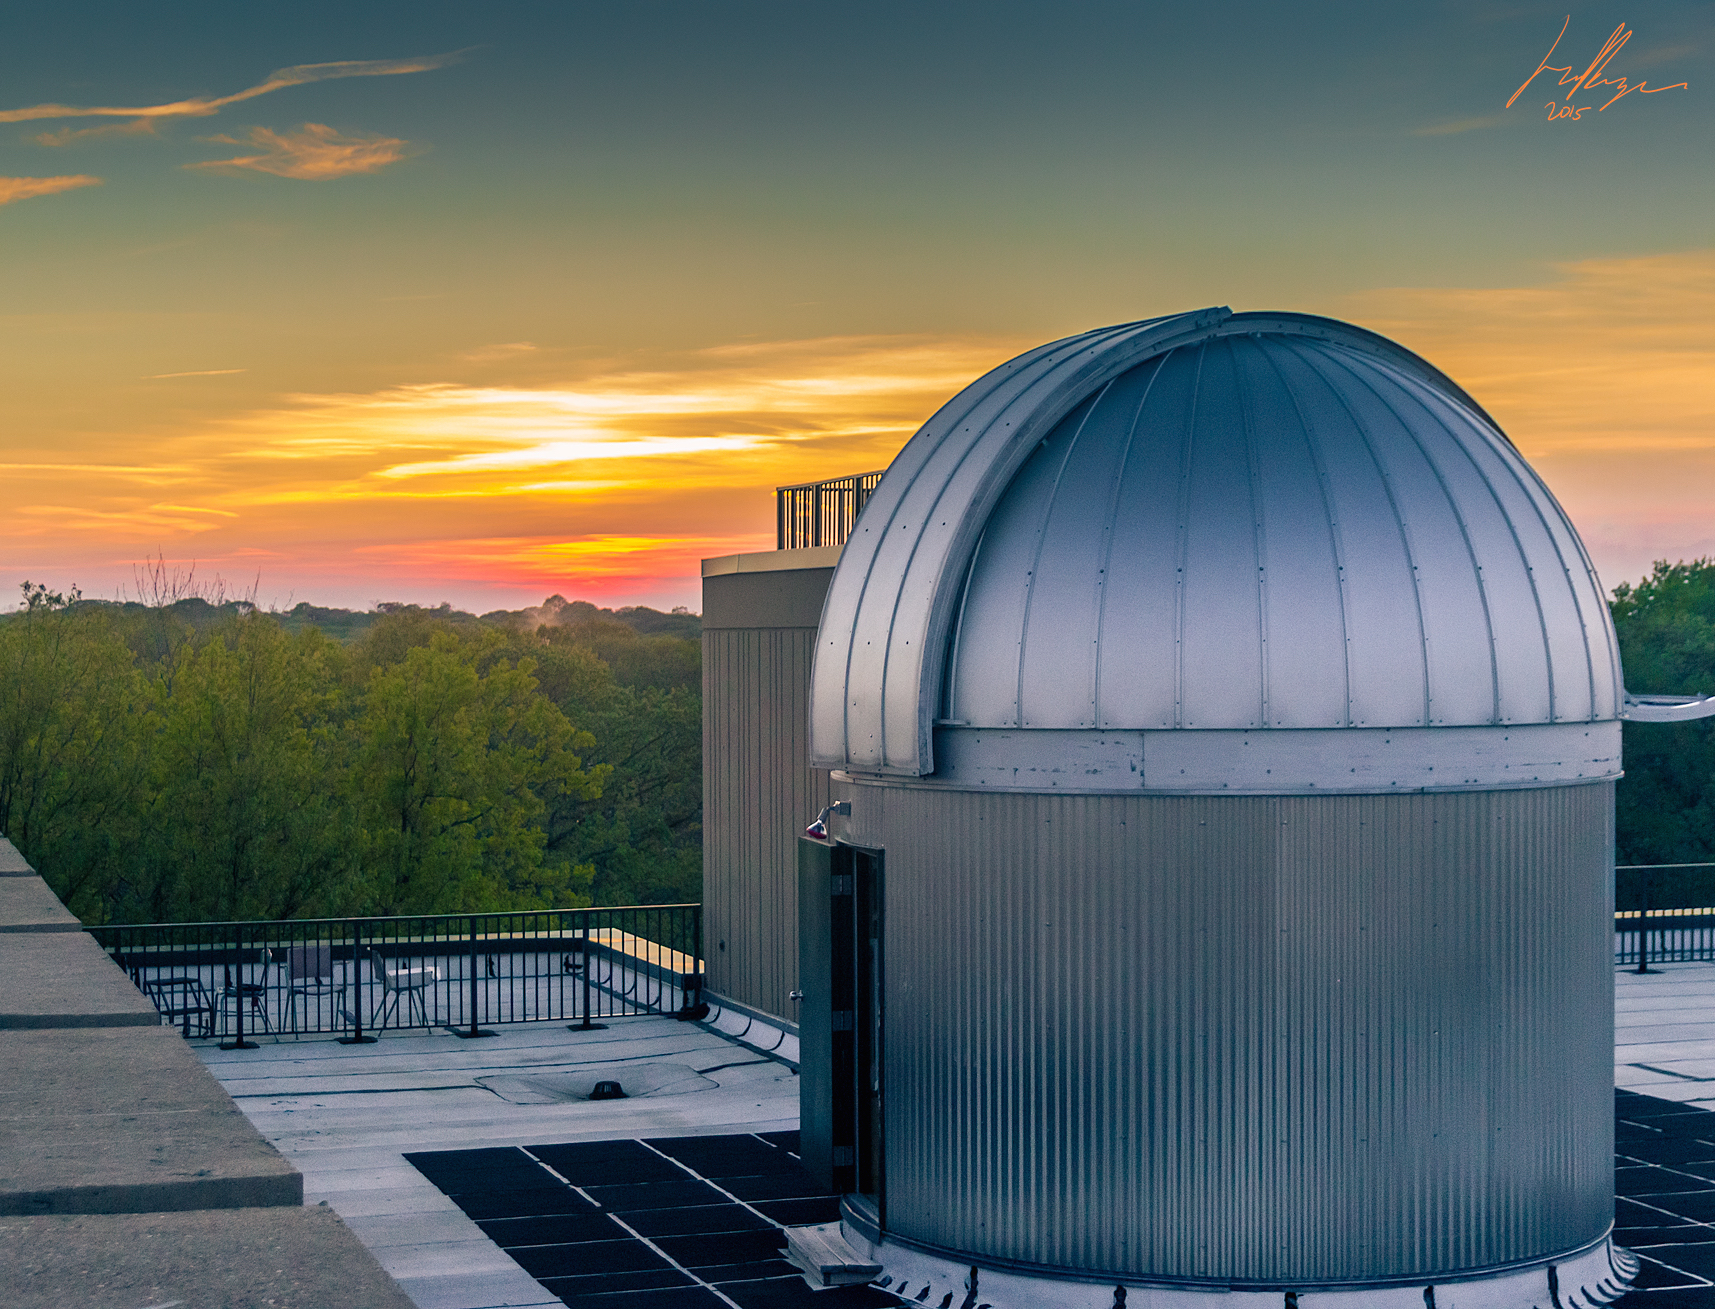
\includegraphics[width=\textwidth]{./images/cover/MtStonyBrookSunset_crop.jpg} 
	\end{center}
\end{figure}
\vspace*{\fill}
\enlargethispage{2.5\baselineskip}
\begin{center}
	Updated \today
\end{center}

\end{titlepage}

%%%%%%%%%%%%%%%%%%%%%%%%%%%%%% Table of Contents %%%%%%%%%%%%%%%%%%%%%%%%%%%%%%

\tableofcontents
\setcounter{tocdepth}{2}
\thispagestyle{empty}
\clearpage

%%%%%%%%%%%%%%%%%%%%%%%%%%%%% Beginning of Manual %%%%%%%%%%%%%%%%%%%%%%%%%%%%%

\setcounter{page}{1}
\section{Introduction}
Mt. Stony Brook Observatory is the Stony Brook University Astronomy Department's facility for astronomy research and pubic outreach.
Located on the roof of the Earth and Space Sciences Building in the center of West Campus, the Observatory is home to a Meade 14" Cassegrain telescope, Celestron 8" Cassegrain telescopes, a Coronado solar refractor, several large-format CCD cameras, spectrographs, and many accessories.
This document is intended to serve as a manual supplementary to the official manuals for each instrument, which can be found at \url{https://sites.google.com/site/stonybrookastronomyclub/mt-stony-brook-observatory}.
It primarily contains instructions specific to the setup of these instruments at Mt. Stony Brook and the maintenance and care for these instruments not otherwise covered by their respective manuals.
It is also intended to be an update to the manual by Wahl and Metchev, 2013 \cite{wahl13} and the much earlier work by Adams, Petreshock, and Wolk, 1995\cite{adams95}.
This manual should be updated when the Astronomy Club or Astronomy Department acquires a new piece of equipment or software or when an older piece of equipment or software becomes deprecated or inoperable.

The site of the Observatory is one of the most light-polluted areas on Eastern Long Island. The absence of directional lighting on campus results in a naked-eye limiting magnitude of 5-5.5. Stony Brook has recently transitioned the majority of outdoor lights on campus to LED, whose broad-spectrum emission may pose a problem when attempting to do spectroscopy. However, the largest light pollution problem is posed by the LeValle Stadium lights; metal-halide lamps which point directly at the Observatory and wash out much of the northern sky. It is recommended that observations of dim targets in the northern hemisphere of the sky be planned around the stadium schedule.


\section{Meade LX200 14'' Telescope}
Mt. Stony Brook's primary telescope is a 14'' f/10 Meade LX200GPS, Schmidt-Cassegrain telescope (affectionately known as "Betsy") that is permanently mounted in the Ash Dome on top of ESS.
It is operated via the Autostar II hand controller, which can issue slew commands and contains a catalog of objects.
The telescope is equipped with a 8x50 finder scope which has a 50mm objective and 8x magnification.
The telescope was installed in 2010 and has accumulated wear and tear.
The gears in the drive motor are worn and will occasionally slip, causing the physical pointing to disagree with the pointing in the Autostar.
The knob to lock the primary mirror is known to come off and is difficult to reattach so it is best to leave the mirror unlocked.
% Is this next bit correct?
When the telescope was assembled, the declination (DEC) setting circle stickers were were placed on the wrong sides. Since the setting circle with the angles labeled can be adjusted independent of the telescope, the angles do not refer to a meaningful DEC.
All directions in this section are given relative to the user looking at the telescope control panel, facing south.
It is recommended that you prop both dome doors open while observing with the LX200 to maintain stable airflow around the telescope, which will improve seeing.
\par There are two default positions that are programmed into the LX200, shown below.
\begin{figure}[H]
    \centering
    \begin{subfigure}[t]{0.5\textwidth}
        \centering
        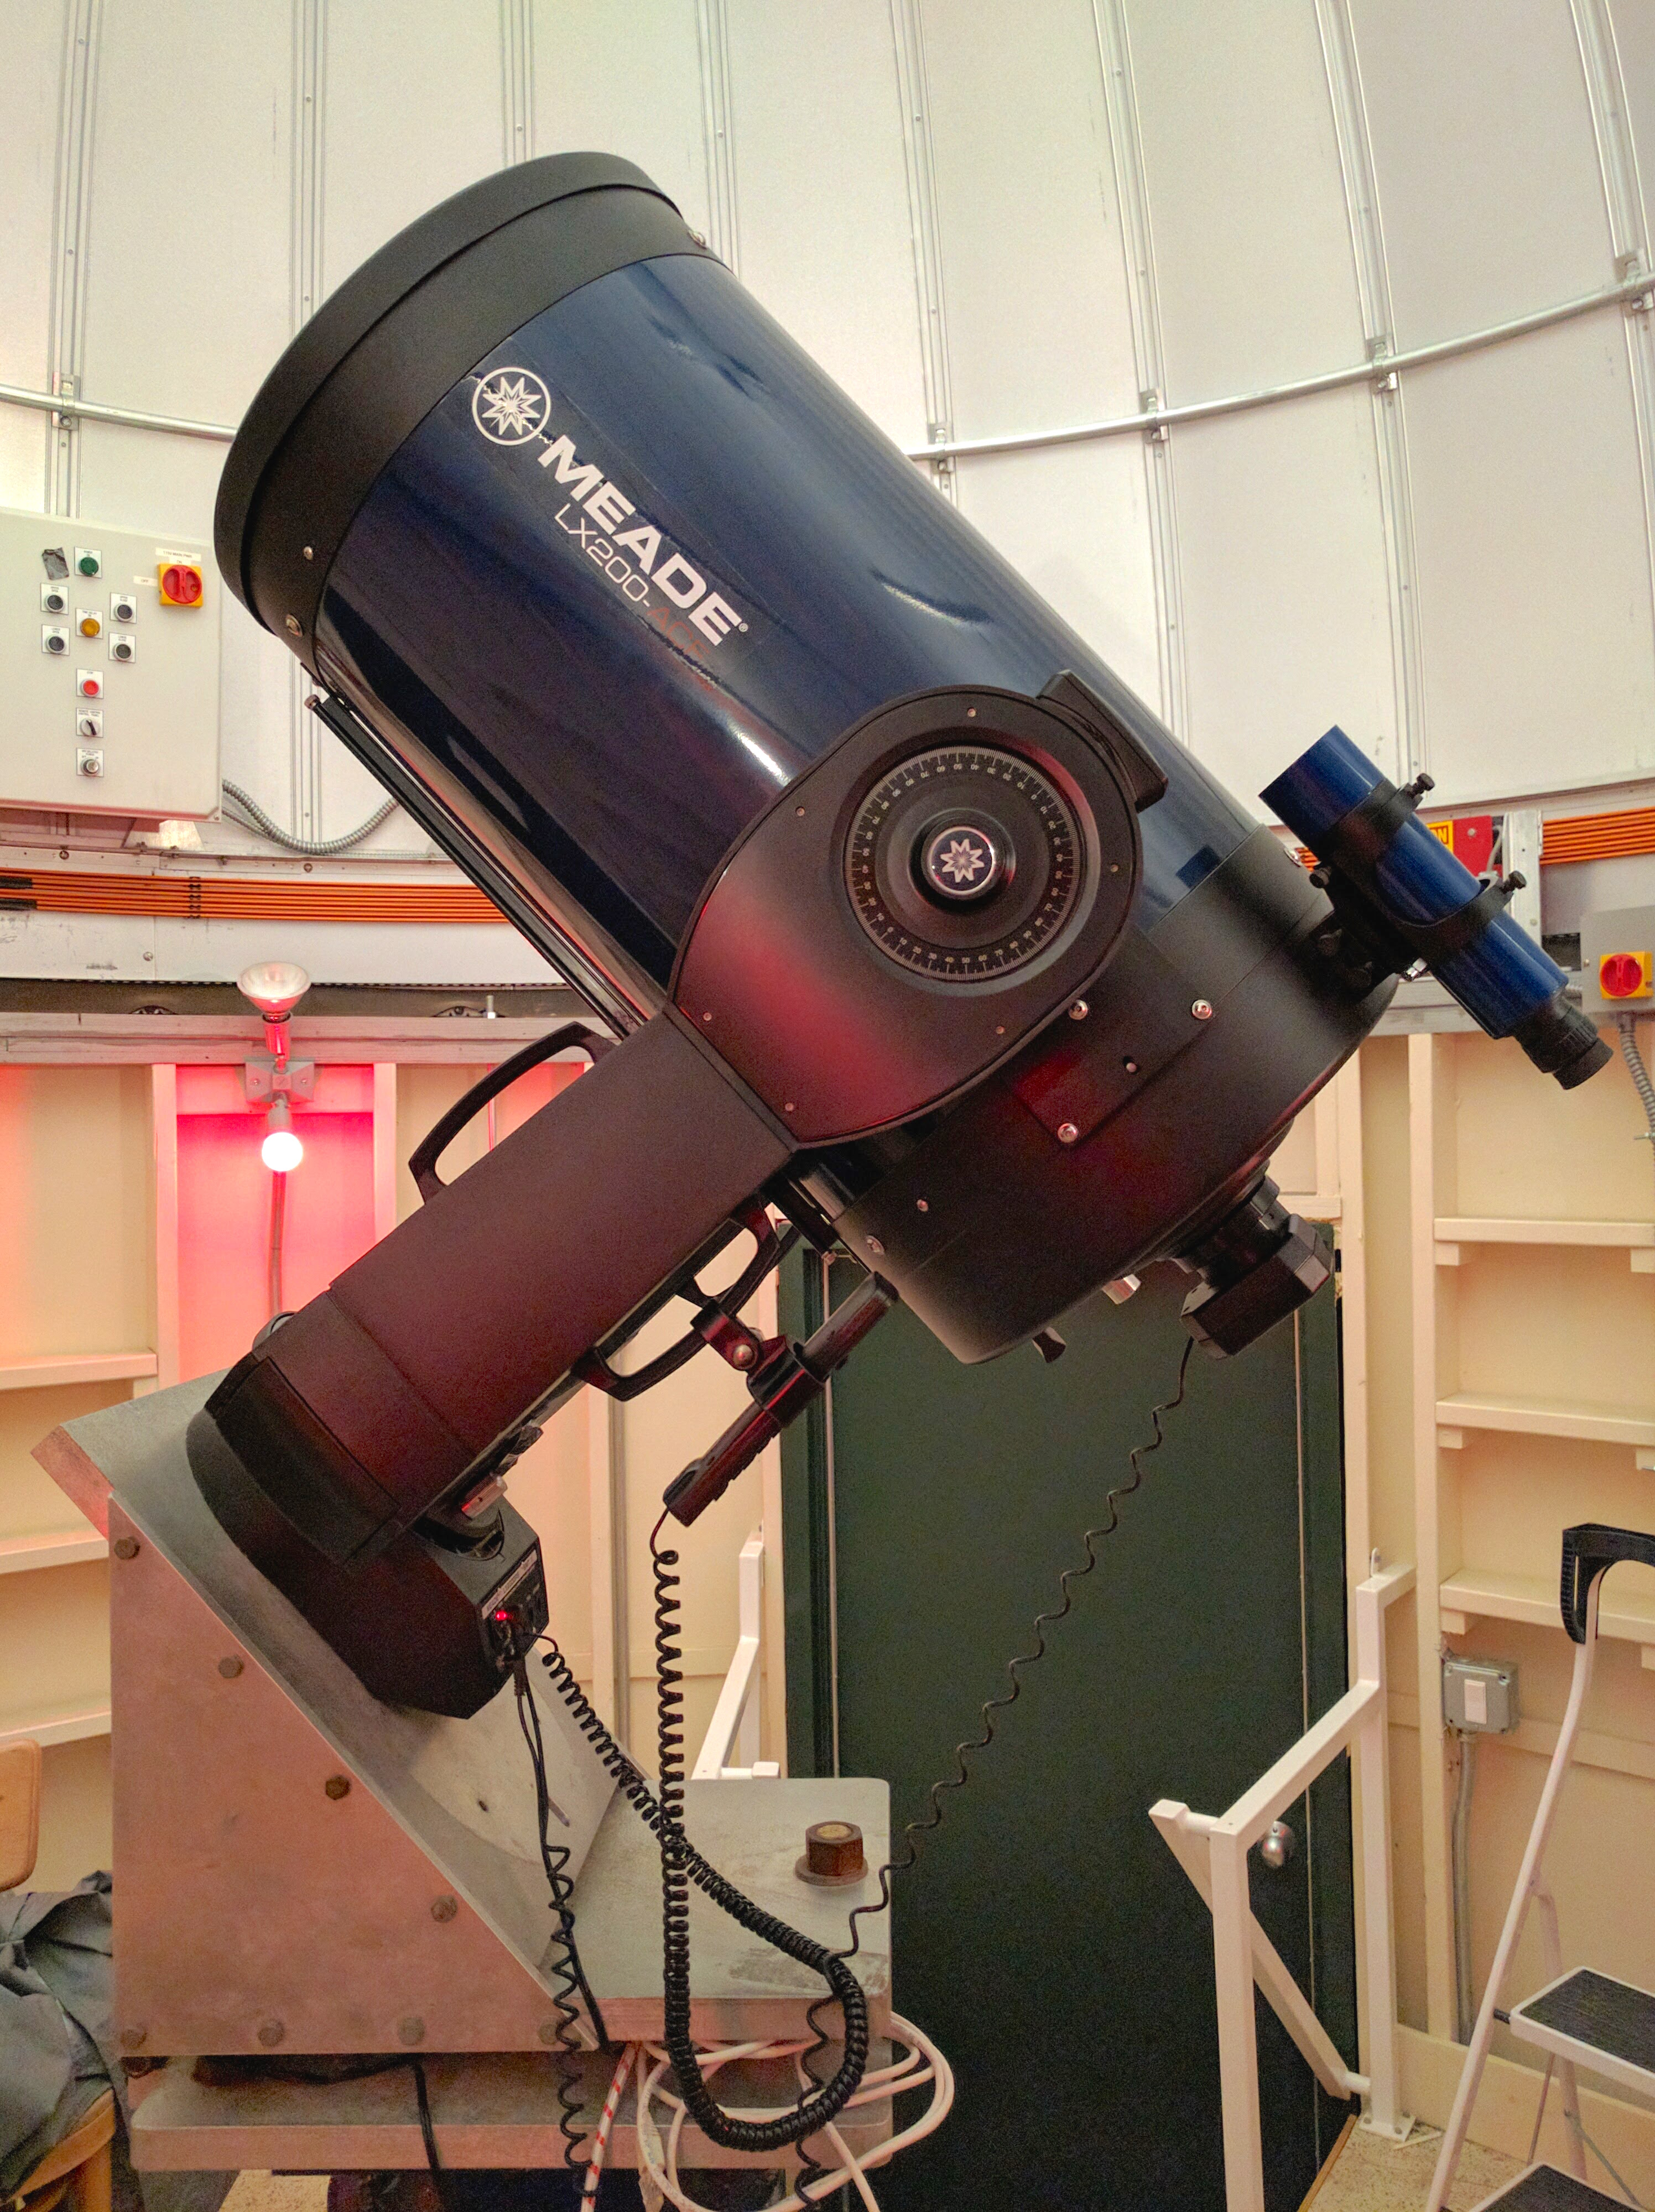
\includegraphics[width=.8\textwidth]{./images/lx200/intro/park_side.jpg}
        \caption{Park position}
    \end{subfigure}%
    \begin{subfigure}[t]{0.5\textwidth}
        \centering
        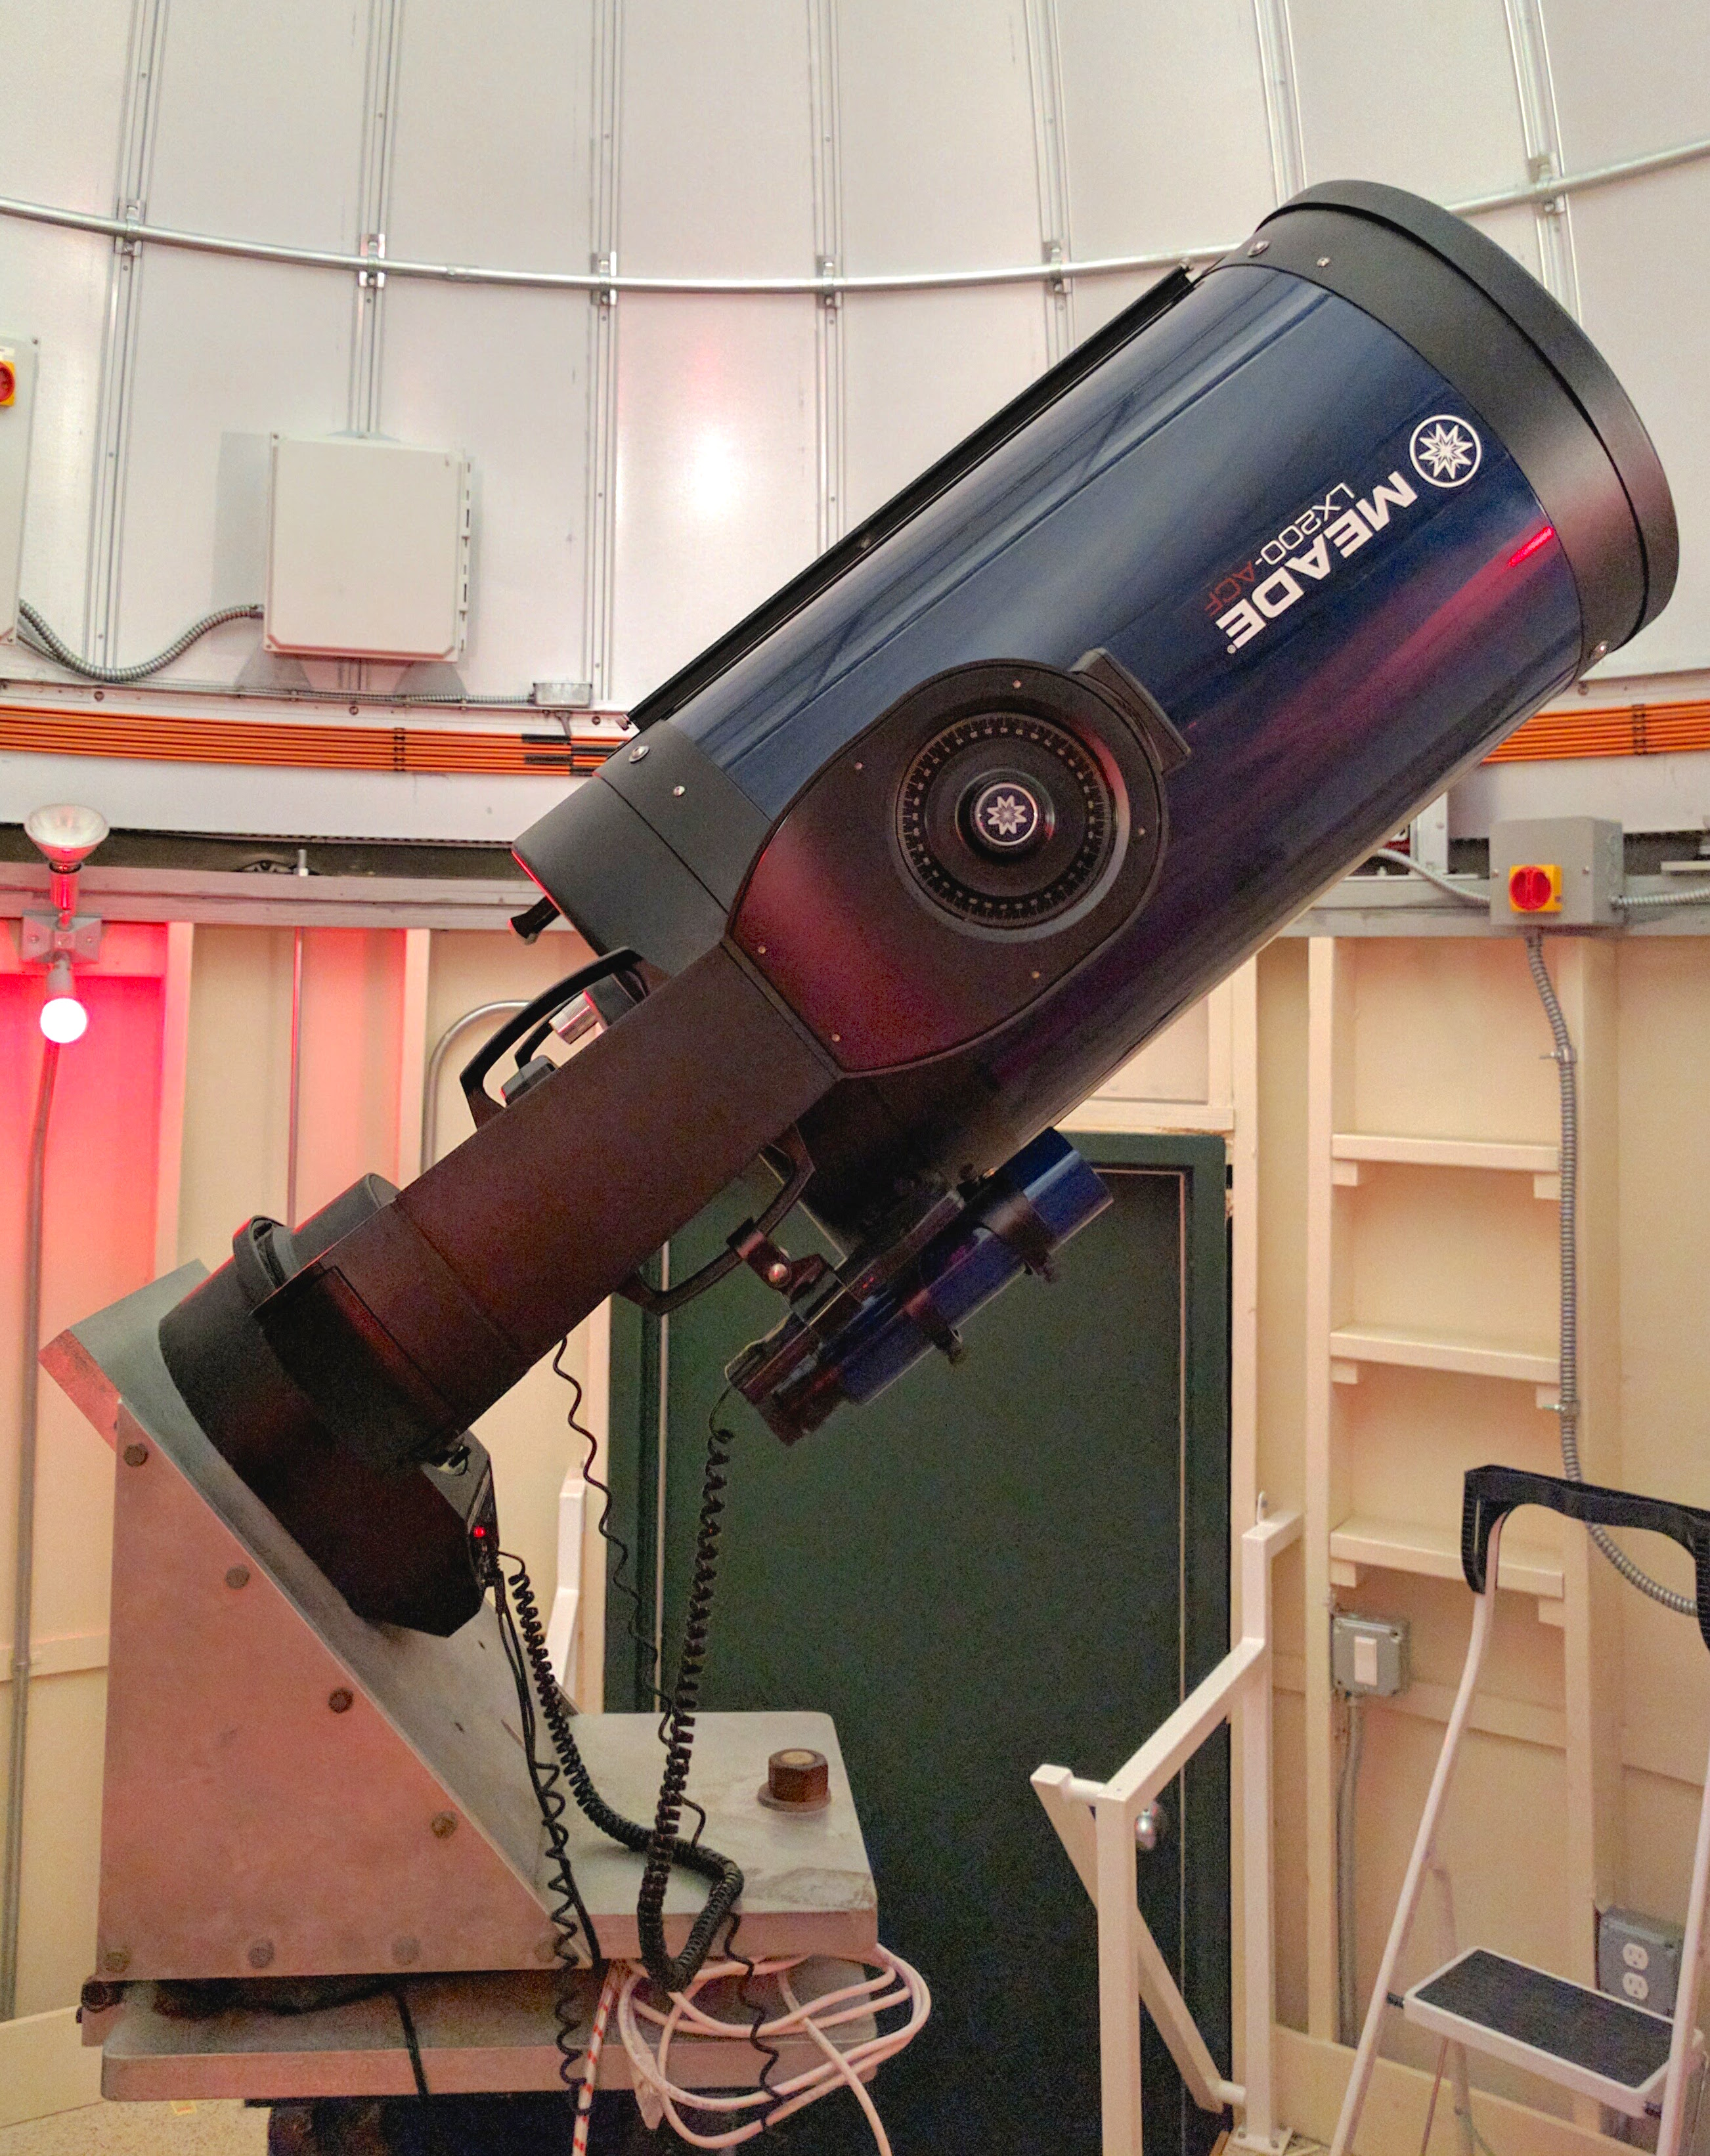
\includegraphics[width=.85\textwidth]{./images/lx200/intro/polarhome_side.jpg}
        \caption{Polar home}
    \end{subfigure}
    \caption{Default positions}
\end{figure}
\noindent When in park position, the telescope is at RA 0h0m0s, DEC 0$\deg$0'0'', pointing due South with the telescope tube parallel to the mount.
This is the position that the telescope should return to when it is parked, before shutting down.
If it does not return to this position, the pointing is likely incorrect.
The polar home position is used during pointing correction, with the telescope at RA 0h0m0s, DEC 90$\deg$0'0'' and the finder scope underneath the telescope tube.

\subsection{Quick Setup Guide (Eyepiece Observing)} \label{ssec:betsy_quick}
The RA and DEC locks on the telescope tube must remain in the LOCKED position at all times. The telescope should be slewed using the Autostar II hand controller.
\begin{enumerate}
	\item Turn on dome drive power (red switch, north side of dome). \label{enum:quicksetup_start}
	\item Open the dome upper shutter by pressing \underline{START}, followed by UPPER SHUTTER OPEN on the dome hand controller (All dome remote commands must be preceded by \underline{START}). If the dome ever loses power and needs to be open or shut manually, refer to Sec. \ref{ssec:dome_trouble}.
\footnote[$\dagger$]{\textbf{Do not open the dome if it is raining, snowing, high winds, or if there is snow accumulation on top of the dome.}}
	\item Open the dome lower shutter by pressing LOWER SHUTTER OPEN on the hand controller
	\item Remove the canvas cover from the telescope.
	\item Gently remove the dust covers from the front of the telescope and finder scope.
	\item Insert 2'' star diagonal and 1.25'' adapter into optical tube. Tighten thumbscrews.
	\item Plug the telescope power cable into the base of the pillar. Turn on the telescope mount (power switch on the RA gearbox).
	\item Wait for telescope to take a GPS fix. For troubleshooting see Sec. \ref{sssec:autostar_trouble}
	\item Insert eyepiece into star diagonal. Tighten thumbscrews.
	\item Ensure primary mirror lock is not engaged (leave the mirror unlocked, the knob has a tendency to fall off).
	\item Slew telescope to a bright object and adjust coarse manual focus knob to bring the object into focus. Fine adjustment can be made with the microfocuser via the Autostar II hand controller.\\[2em]
	\label{enum:quicksetup_end}
	\textbf{\begin{center}
	Shutdown Procedure:
	\end{center}}
	\item \textbf{Park the telescope.\footnote[*]{DONT FORGET TO PARK THE TELESCOPE!!!}} Failure to do so will result in incorrect pointing the next time it is powered up. From the Autostar II hand controller:\\
Select Item:
	\item[]\quad $>$Utilities
	\item[]\quad\quad $>$Park Scope
	\label{enum:quickshutdown_start}
	\item Power off telescope
	\item Remove eyepiece from star diagonal
	\item Remove star diagonal from telescope tube
	\item Replace the dust covers on the front of the telescope and finder tube
	\item Replace canvas cover over telescope
	\item Rotate the dome so that the slit is over the south entrance door
	\item Close the dome lower shutter
	\item Close the dome upper shutter
	\item Write an observing log book entry with the observer's names, date/time in, date/time out, what you observed, any issues
	\item Turn off dome drive power
	\label{enum:quickshutdown_end}
\end{enumerate}


\subsection{Autostar II Hand Controller}
The Autostar II is the primary control interface for the operation of the LX200.
The data is not stored in the Autostar, but in the base of the telescope.
The current firmware version is V4.2g.
The buttons on the Autostar and their functions are identified below.

\begin{figure}[H]
	\begin{center}
		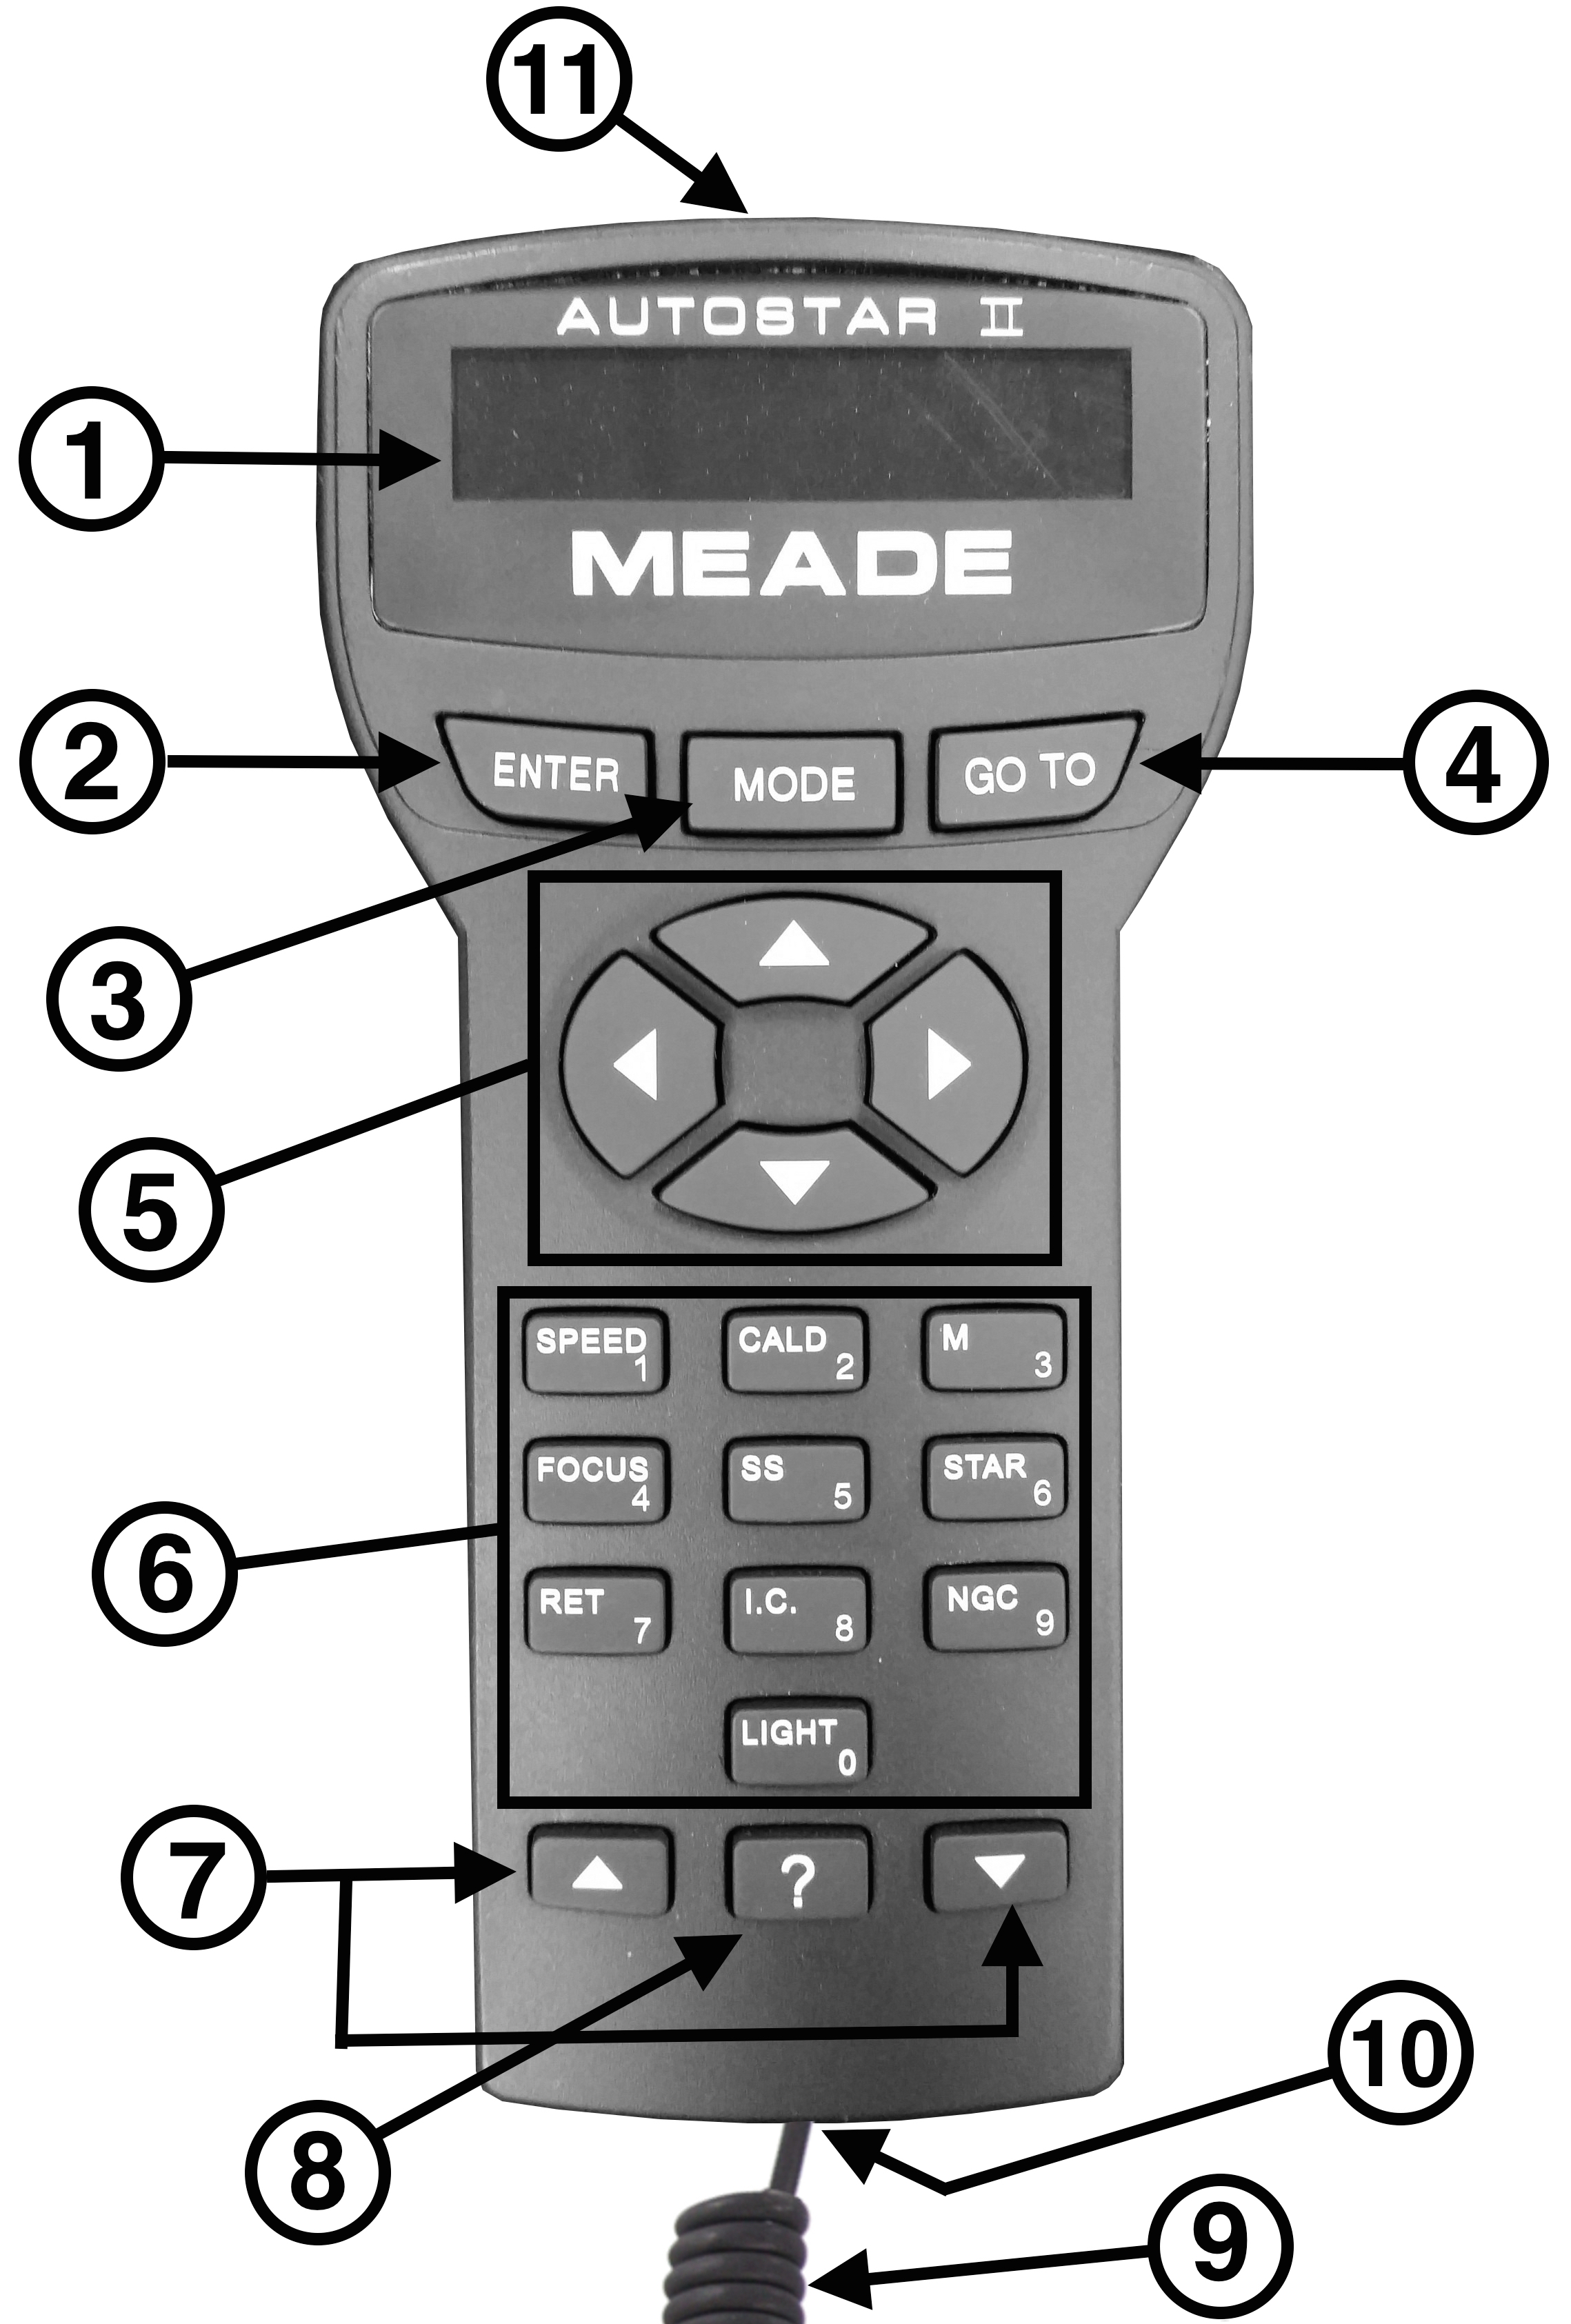
\includegraphics[width=.6\textwidth]{./images/lx200/autostar/controller_labeled.jpg}
	\end{center}
\end{figure}

	\begin{enumerate}[label=\protect\circled{\arabic*}]\small
	\item LCD display
	\item ENTER Key: Descend menu level or select option \par
			\textit{Press and hold for 2 seconds to sync on
					selected object.}
	\item MODE Key: Ascend menu level\par
			\textit{Press and hold for 2 seconds to display 
			telescope status. Press scroll keys to display:
			\begin{itemize}[itemsep=0pt]
				\item RA and DEC coordinates
				\item Alt. and Az. coordinates
				\item Local and Local Sidereal Time
				\item Timer and Alarm status
				\item Date
				\item Site coordinates
				\item Battery status		
			\end{itemize}												
			}
	\item GOTO Key: Slew to coordinates of selected object. Press any other key to abort.
	\item Arrow Keys: Up and down keys slew the telescope in DEC. Left and right keys in RA.
			In any data entry screen, up and down keys scroll through A-Z, 0-9. Left and right
			move cursor between characters.
	\item Number keys: Enter digits 0-9 in any data entry screen. Each number key also has a
			specific function, described further below:
			\begin{itemize}[itemsep=0pt]
				\item[] \textbf{[1] SPEED:} Adjust slew speed of telescope
				\item[] \textbf{[2] CALD:} Display Caldwell catalog library
				\item[] \textbf{[3] M:} Display Messier catalog library
				\item[] \textbf{[4] FOCUS:} Adjust microfocuser speed
				\item[] \textbf{[5] SS:} Display Solar System object library
				\item[] \textbf{[6] STAR:} Display Star object library
				\item[] \textbf{[7] RET:} Display Retical Control menu
				\item[] \textbf{[8] IC:} Display Index catalog library
				\item[] \textbf{[9] NGC:} Display New General Catalog library
				\item[] \textbf{[0] LIGHT:} Toggle on/off red utility light on top of handbox
			\end{itemize}
	\item Scroll keys: Scroll through menu options. Also controls scroll speed of tickertape
			dialogue.
	\item ? Key: Display help file for active task. Press MODE to exit.
	\item Autostar II cable: Other end of cable plugs into HBX port on telescope control panel.
		There is a spare cable in the telescope room, but in a pinch you can use a regular 4-pin
			handset cable from one of the professor's office phones.
	\item Autostar II cable port
	\item Utility Light: built-in red light
	\end{enumerate}


\noindent\textbf{Syncing:} To improve the telescope pointing accuracy in one region of the sky, sync on a bright star.
Note: This may decrease pointing accuracy in other regions of the sky. Never sync on Solar System objects.
\begin{enumerate}
	\item Select a bright star from the star menu\\
	Select item: $>$ Objects $>$ Star
	\item Center the star in the FOV.
	\item Press and hold ENTER for 2 seconds.
	\item Press ENTER to sync.
\end{enumerate}
\textbf{Current Pointing:} To view your current pointing in RA and DEC coordinates, press and hold MODE for 2 seconds.\\

\noindent\textbf{Slew Speeds:} There are nine slew speeds available to the Autostar, listed below.

\begin{center}  
\small{
\begin{tabular}{ccc}
Number Key	& Autostar Description	& Rate\\
\hline
1			& 1x				& 9.9 arcsec/s (0.66*sidereal, default)\\[-1ex]
2			& 2x				& 0.5 arcmin/s\\[-1ex]
3			& 8x				& 2 arcmin/s\\[-1ex]
4			& 16x			& 4 arcmin/s\\[-1ex]
5			& 64x			& 16 arcmin/s\\[-1ex]
6			& 128x			& 30 arcmin/s\\[-1ex]
7			& 1.5$\deg$		& 1.5$\deg$/s\\[-1ex]
8			& 3$\deg$		& 3$\deg$/s\\[-1ex]
9 			& Max			& 8$\deg$/s

\end{tabular}}\\
\captionof{table}{Autostar II slew speeds}
				\label{tab:slew_speeds} 
\vspace{.4 cm}
\end{center}


\subsubsection{Computer Connection}
The Autostar is programmable, to a certain degree, using the Meade Autostar software suite, which includes ASU (Autostar Updater) and AutoStar Observatory. 
This software is installed on the Department laptop.
From ASU, the Autostar firmware can be update, custom user objects managed, and custom tours added.
From AutoStar Observatory, the telescope can be slewed via computer serial control.
\par The cable to connect the laptop to the telescope is a USB-to-RS232-to-6-pin cable.
There is a spare on the top shelf with the eyepieces in the telescope room.
Plug the USB end of the cable into the laptop and the 6-pin end into the RS232 jack on the telescope's computer control panel.
Ensure that the Autostar is plugged into the HBX jack.

\begin{figure}[H]
	\begin{tikzpicture}
    
    \begin{scope}[xshift=-1mm, yshift=0cm]
    \node {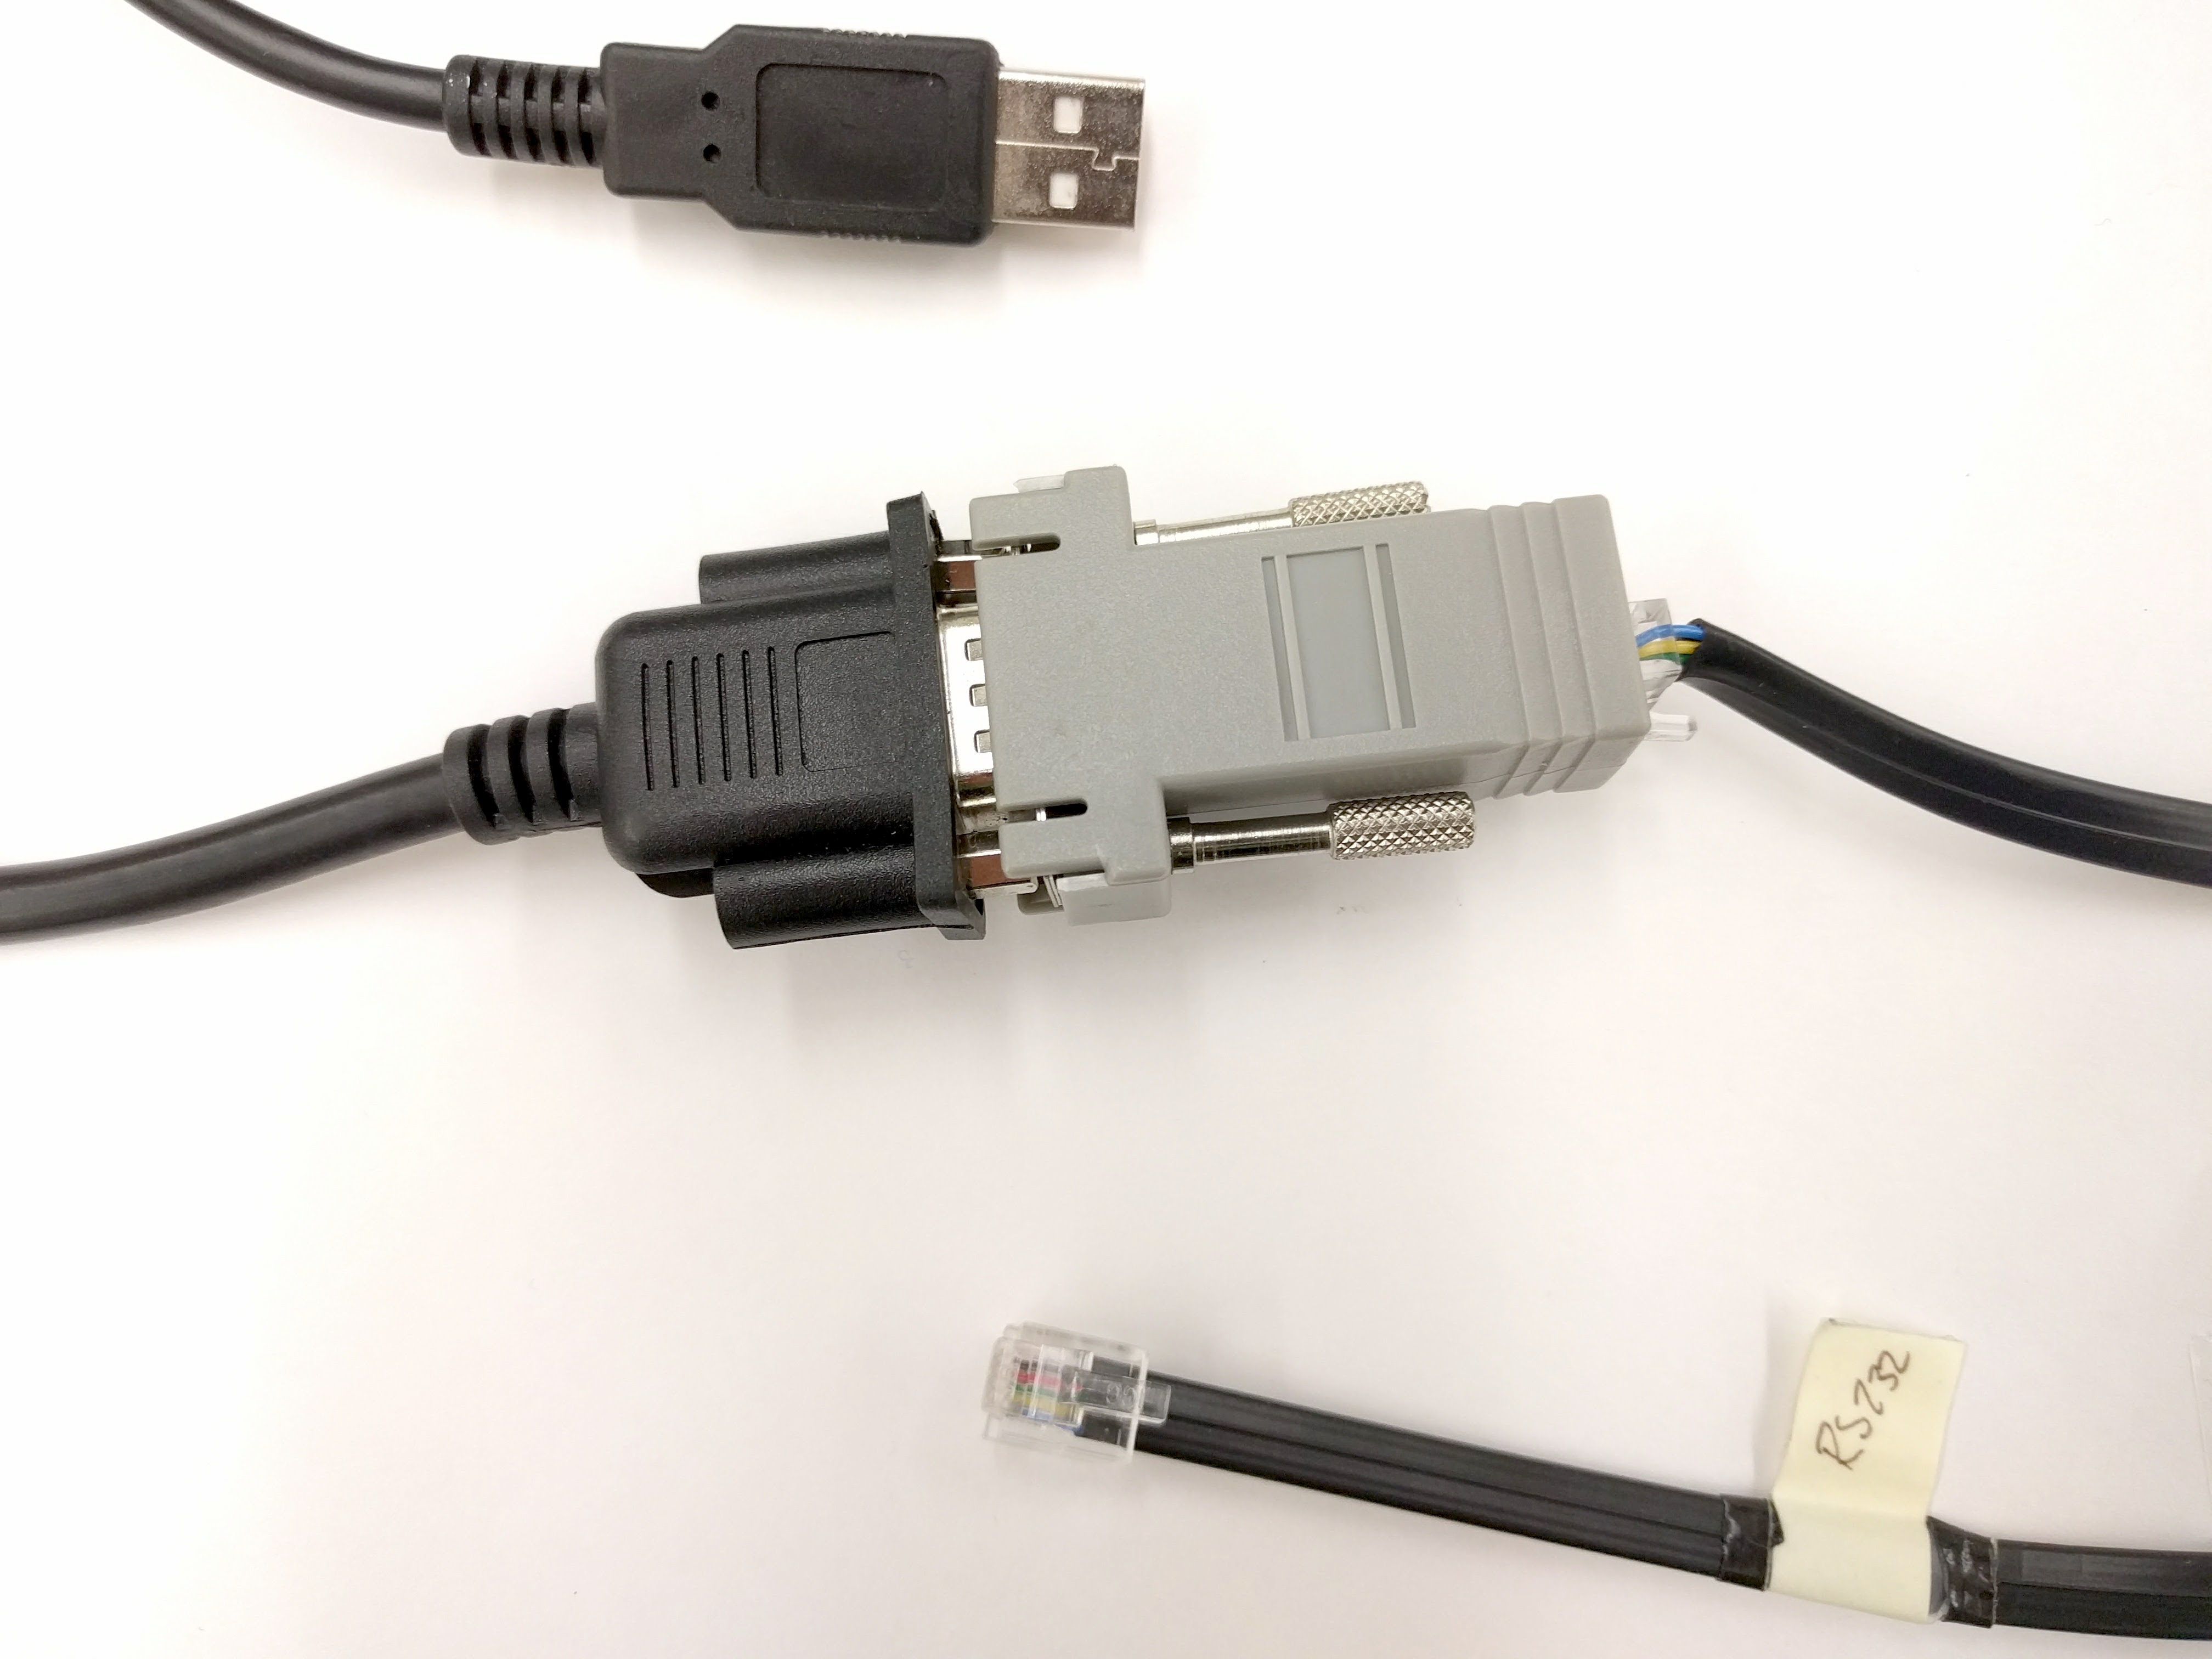
\includegraphics[width=.45\textwidth]{./images/lx200/computer_ctrl/usb_to_RS232.jpg}};
    \end{scope}    
    
    \begin{scope}[xshift=.5\textwidth, yshift=0]
    \node {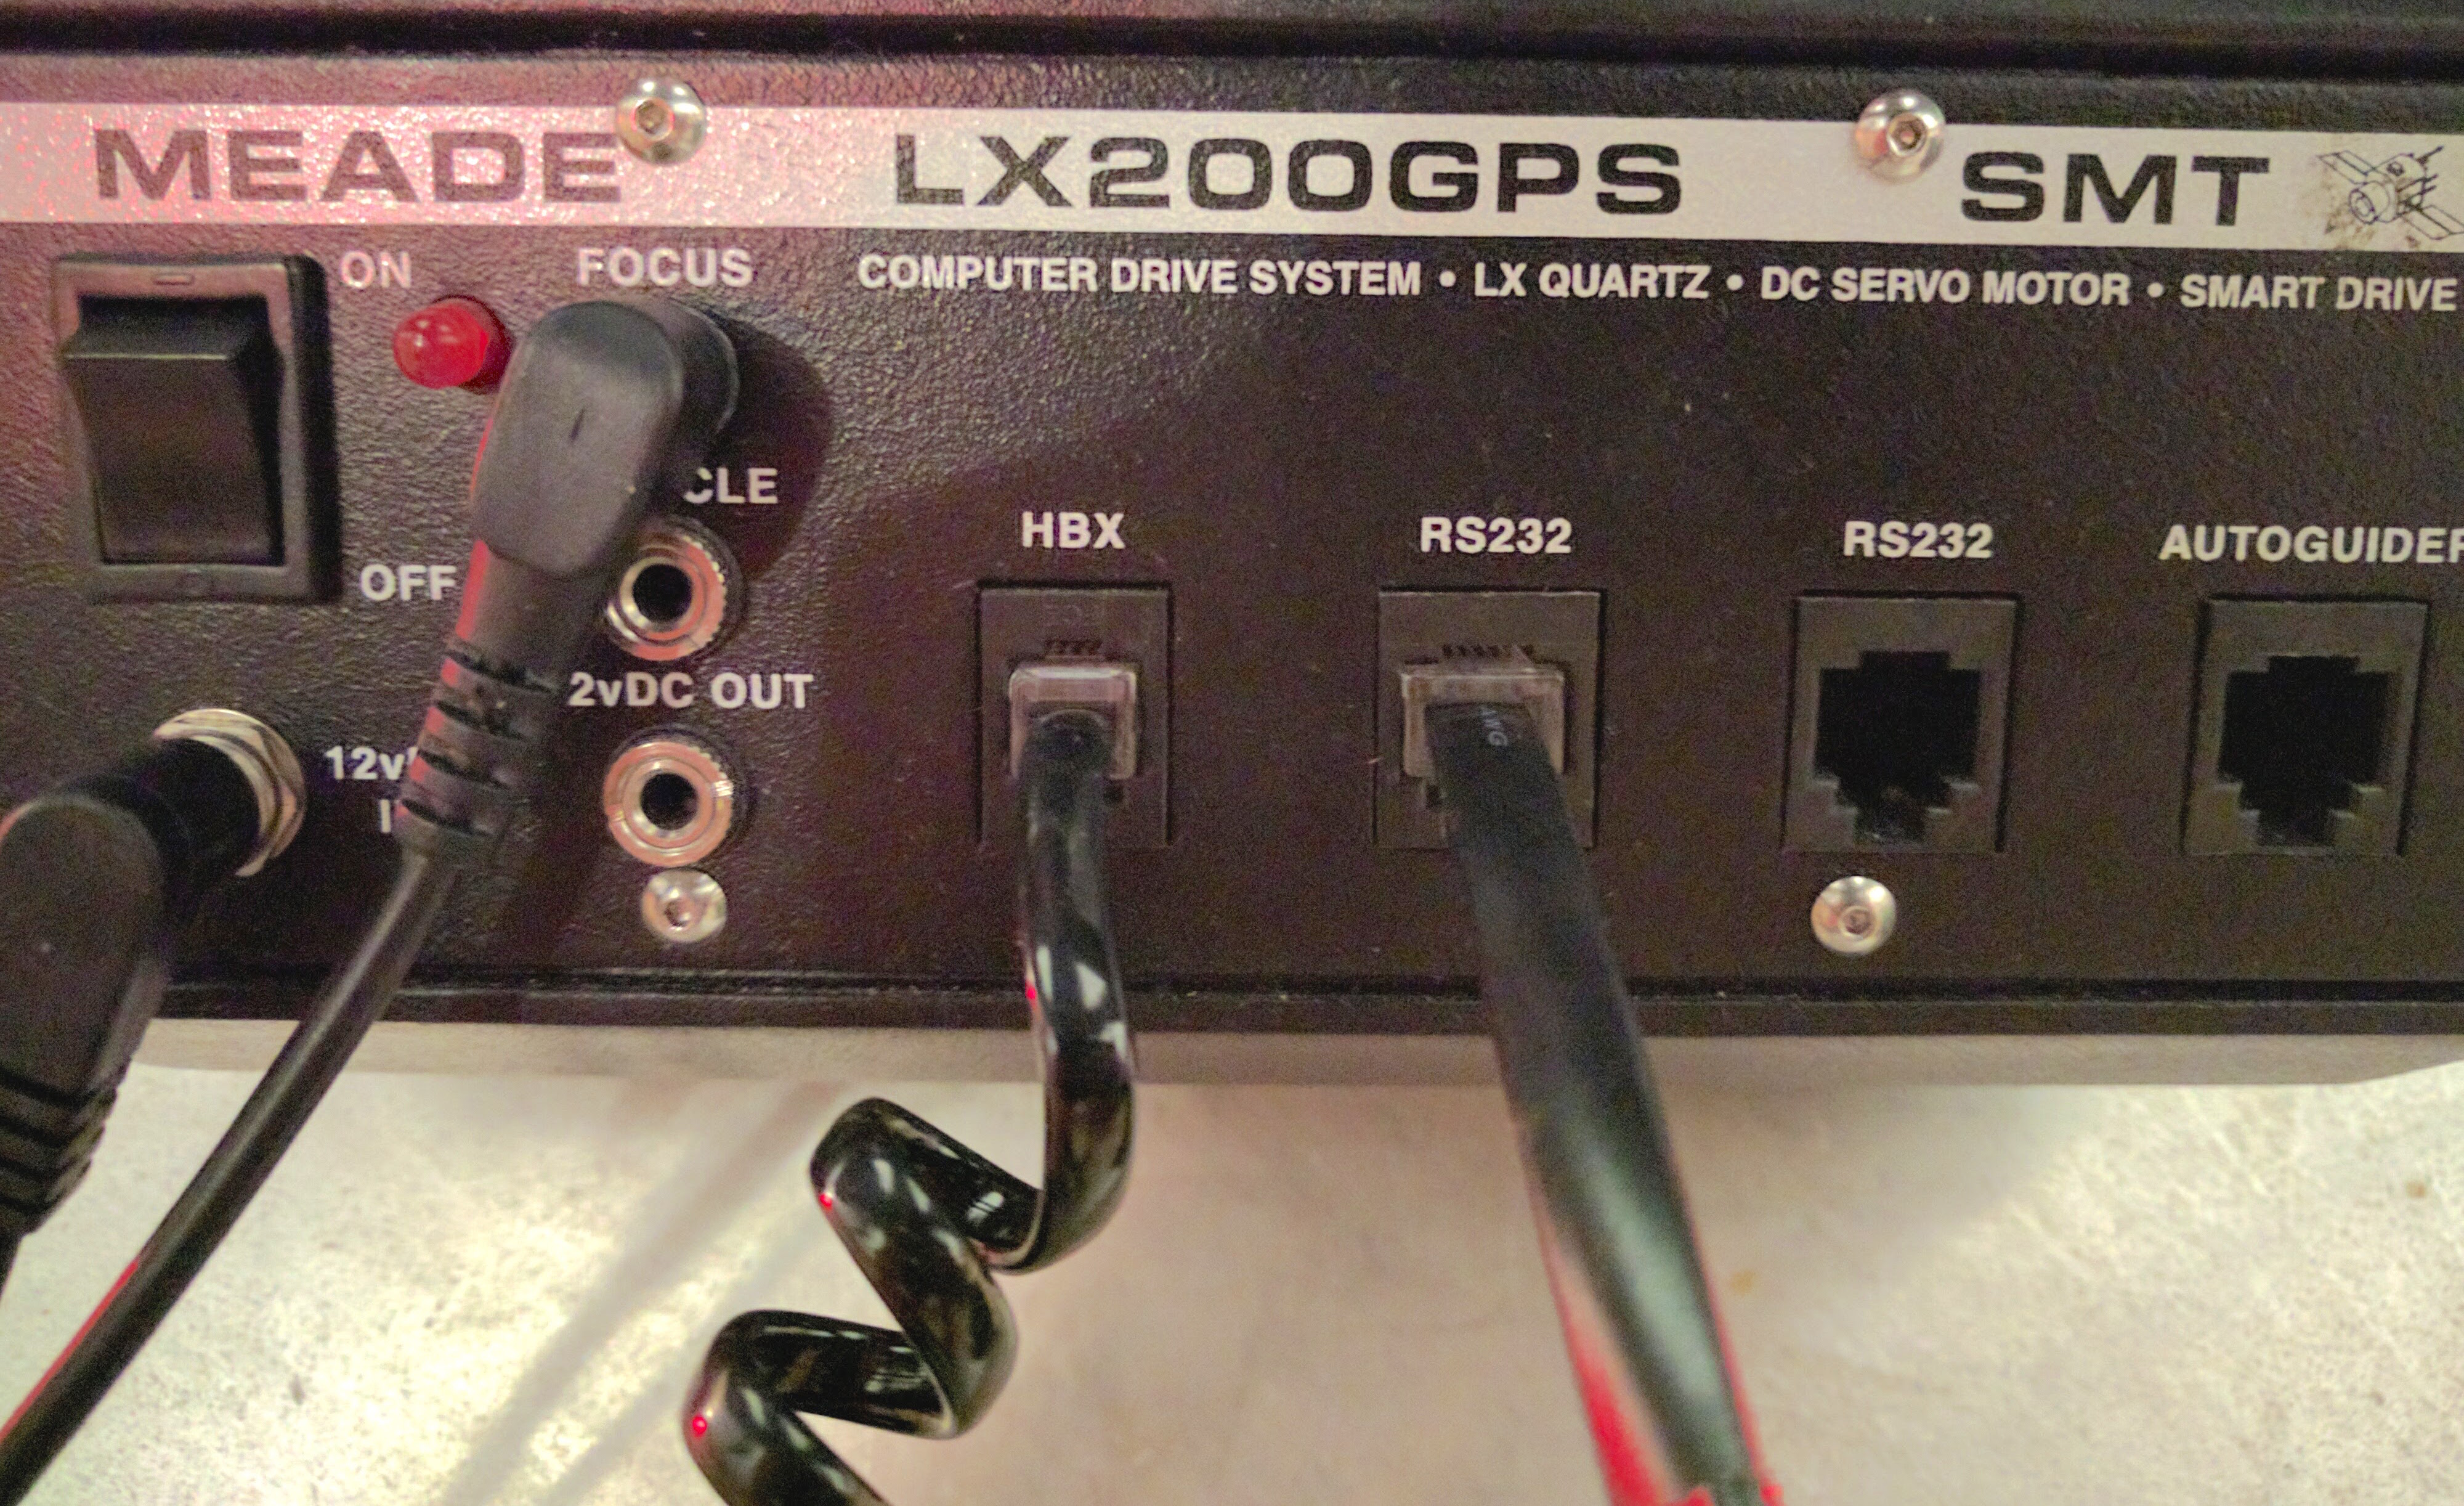
\includegraphics[width=.55\textwidth]{./images/lx200/computer_ctrl/computer_drive_panel.jpg}};
    \end{scope}
    
	\end{tikzpicture}
\end{figure}


\subsubsection{Managing Custom User Objects}
The current version of Autostar Software includes over 145,000 objects in its database.
However, some dimmer objects are not included and you may want to add them to the database if their RA and DEC are known.
There are two methods for managing custom user objects, the first of which uses the hand controller directly:
\begin{enumerate}
	\item[] Select item:
	\item[]\quad $>$Object
	\item[]\quad\quad $>$User Object
	\item[]\quad\quad\quad $>$Select
	\item[]\quad\quad\quad $>$Add
	\item[]\quad\quad\quad $>$Delete
	\item[]\quad\quad\quad $>$Edit
\end{enumerate}
To add an object:
\begin{enumerate}
	\item[]\quad\quad\quad $>$Add
	\item[]\quad\quad\quad\quad $>$Enter object name using the menu navigation and number keys.
	To move between characters, use the slew-left and slew-right keys. Press ENTER.
	\item[]\quad\quad\quad\quad $>$Enter object RA in the same fashion. Press ENTER. 
	\item[]\quad\quad\quad\quad $>$Enter object DEC in the same fashion. Press ENTER.
	\item[]\quad\quad\quad\quad $>$Optional: Enter the object's angular size in 
	min. Press ENTER.
	\item[]\quad\quad\quad\quad $>$Optional: Enter the object's magnitude. Press ENTER.
\end{enumerate}
To slew to a User Object:
\begin{enumerate}
	\item[]\quad\quad\quad $>$Select
	\item[]\quad\quad\quad\quad $>$Select the desired object and press ENTER.
	\item[]\quad\quad\quad\quad $>$The object name and its coordinates will appear. Press GOTO.
\end{enumerate}
If there are many User Objects stored in the Autostar, many of which are not in use or do not have meaningful names, the method using the ASU suite is desired:
\begin{enumerate}
	\item Launch ASU from the laptop
	\item Connect the RS232 end of the computer interface cable into the corresponding jack on telescope's computer control panel and the USB end into the laptop.
	\item In ASU, click "Connect". "Model: LX200 GPS\quad Handbox Ver:4.2g" should appear at the bottom of the window.
	\item Click "Retrieve".
	\item All User Objects will be listed in the AutoStar panel under the User Objects tab.
	\item To Add, Edit, or Delete a User Object, right-click on the object, select the desired option, and fill in the objects information.
	\item Once all changes have been made, click "Send". Note: This will replace the AutoStar hand controller library with the ASU library.
\end{enumerate}

\subsubsection{Custom Tours}
Autostar tours enable the user to slew to multiple pre-determined objects in sequence without having to search through the Autostar's database.
Tours are ideal for Open Nights and other outreach events where the target objects are planned in advance.
They also allow the user to display custom information on the Autostar LCD while the tour is running,
Tours are written in .txt files and uploaded to the Autostar via the ASU software.
A guide to the tour syntax can be found in Appendix C of the LX200 Manual \cite{lx200}.
To upload a tour to the Autostar:
\begin{enumerate}
	\item Launch ASU from the laptop
	\item File $>$ Import
	\item Select the .txt file containing your tour. Set object type to "Tour". Click "Import".
	\item The tour will appear in the left "Library" panel of ASU.
	\item Connect the laptop to the the telescope. Click "Connect" in ASU.
	\item Click "Retrieve". This will add the Autostar library to the ASU library.
	\item Select the tour you want to add and click "Selected -$>$".
			If a tour with the same name already exists on the Autostar, you will be prompted to replace it with the one in your library.
			The tour will appear in the "AutoStar" panel of ASU.
	\item Click "Send". Note: This will replace the AutoStar hand controller library with the ASU library.
\end{enumerate}
To run a tour on the telescope:
\begin{enumerate}
	\item To initiate the tour on the Autostar press Select item $>$ Guided Tour.
	\item Navigate the list of tours and select the one you want to run by pressing ENTER.
	\item If an object has set or is not yet risen, the tour will automatically skip to the next object
	\item Press GOTO on an object to slew to it
	\item To exit the tour at any time press and hold MODE for 2 seconds.
\end{enumerate}
Sample tours can be found at \url{http://www.astro.sunysb.edu/astro/astroclub/Mt_Stony_Brook/AutostarII_Tours}.

\subsubsection{Autostar Troubleshooting}\label{sssec:autostar_trouble}
\textbf{\flushleft Issue:} The Autostar displays "TAKING GPS FIX" and nothing happens or displays "COULD NOT FIND GPS FIX"\\
\textbf{Solution:} Sometimes the telescope has difficulty taking a GPS fix if there is not a clear line-of-sight between the GPS antenna and the southern sky. Make sure the dome shutters are open. Rotate the dome so that the slit is pointing south and slew the telescope so that it is pointing westward. The fork arm with the antenna will be pointing south. 

\textbf{\flushleft Issues:}
\begin{itemize}
	\item The hand controller display gets dim or characters flicker or disappear.
	\item The hand controller is unresponsive to button presses
\end{itemize}
\textbf{Solution:} The Autostar display is an LCD which is known to dim in temperatures below 27$\deg$ F (-3 C) and fail altogether if exposed to such temperatures for more than 20 minutes, especially in high humidity. This is not permanent. Keep the hand controller inside your pocket while observing in especially cold conditions.

\textbf{\flushleft Issue:} The Autostar does not respond to slew commands during alignment\\
\textbf{Solution:} When performing an alignment, the Autostar will slew the telescope to a nearby bright star. Once the alignment star is reached, the Autostar allows the user to correct the pointing by centering the star in the eyepiece, but assumes that the telescope pointing is nearly correct. The Autostar automatically sets the slew rate to the lowest setting "2x" (0.5 arcmin/s). When issuing slew commands at this rate it may appear that the telescope is not responding when in fact it is moving very slowly.


\textbf{\flushleft Issues:} Telescope pointing for solar system objects is off by as much as 0.5\deg\\
\textbf{Solution:}
Since solar system objects are relatively close to Earth, their positions in the sky are known with less precision. This may seem counter-intuitive but closer objects have more complicated sidereal motion (relative to background stars). Small errors in telescope alignment are magnified when calculating positions of these objects. That is why you should avoid syncing the telescope on solar system objects.

\section{SBIG STL-1001E CCD Camera}
\subsection{Quick Setup Guide (CCD + LX200)}
Find, focus, binning, etc.
\subsection{Changing the Filter Wheel}


\section{MallinCam Xtreme II}
The MallinCam Xtreme II is the Astronomy Club's color-video CCD camera.
The camera houses an extremely sensitive Sony X418AKL sensor and provides deep images with very short exposure times, especially when combined with a focal reducer.
This makes it an ideal tool for public outreach, allowing the operator to display images or video in "real time".
A major downside of the camera is that it outputs an analog video signal (which degrades with increasing cable length) so a conversion to HDMI is preferred if using a display monitor that is not mounted on the scope.
\textbf{Do not use power cable that is coupled with the composite video cable}.
Since the cables are not individually shielded, the power cable may induce a current in the video cable leading to rolling bars in the image.
The lack of a raw digital output also means that the scientific capabilities of the instrument are limited.
\par The camera contains a Peltier cooling system capable of cooling the sensor down to 26 C below ambient (unfortunately the camera does not give a temperature readout), greatly suppressing the thermal noise typical in such sensitive chips.
This also means that dew and frost have a tendency to condense on the sensor when operating at the highest cooling levels in high humidity conditions.
It is highly recommended that you read Section \ref{sssec:dew} on Dew and Frost Prevention before operating in such conditions.
\par The camera can be controlled by either the navigation keys on the back of the camera, a wireless Bluetooth remote, or by a computer running Miloslick MallinCam control software.
For detailed descriptions of the software menus and settings, refer to the Miloslick MallinCam control user's guide\cite{miloslick}.
Upon launching the software you may be prompted to update.
\textbf{Do not update MallinCam Miloslick software when prompted.}
Always click "Skip this version", otherwise you will have to purchase another activation key in order to continue using the updated software.
\par The MallinCam was purchased with an MFR-5 focal reducer, specifically designed for the MallinCam XII.
The focal reducer can provide between 0.3x and 0.8x reduction, depending on the configuration.
Refer to Appendix \ref{sssec:focal_reduction} for specifications of each configuration.
\par For a more detailed description of camera settings, components, and recommended settings refer to MallinCam's official Xtreme manual\cite{mallincam}. 
For any issues with the MallinCam including replacement parts, hardware failures, and general questions, contact Jack Huerkamp at MallinCamusa@gmail.com.
%% Image of ports, cables, and accessories here
%% Insert FOV for each combination of focal reducer and telescope and spacer
%% Take images of jupiter in all configurations FOV = (px width of image / px width of jupiter) x angular size jupiter



\begin{longtable}[t]{cc}
	\multicolumn{1}{m{.4\textwidth}}{
		\begin{enumerate}[label=\protect\circled{\arabic*}]\small
		\item Video Out (BNC)
		\item 12V Power in
		\item Red Power on LED
		\item SVideo in (S-VHS)
		\item Auto iris select switch
		\item Computer control input (RS232)
		\item Enter Key
		\item Up Arrow
		\item Down Arrow
		\item Left Arrow
		\item Right Arrow
		\end{enumerate}}

	&		
		
	\raisebox{-.5\totalheight}{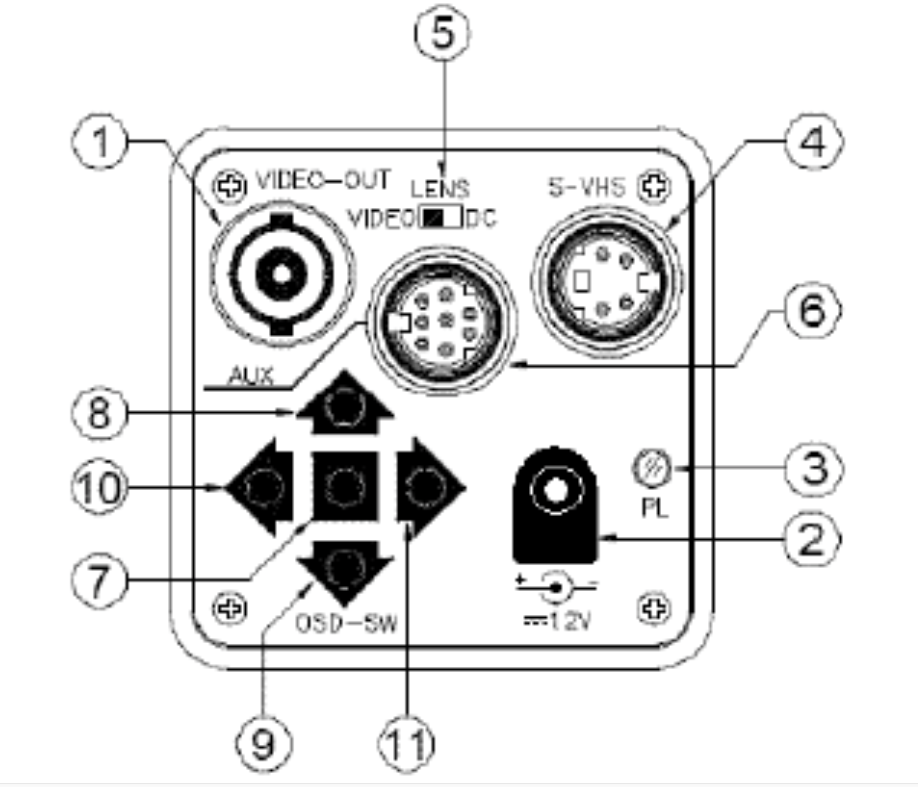
\includegraphics[width=.6\textwidth]{./images/MallinCam/overview/x2_back.png}}
\end{longtable}   

\subsection{Astrofest Setup\\
\small(MallinCam with Miloslick Control + Meade LX-200 + TV)} \label{ssec:Astrofest_Setup}
This setup configuration is ideal for outreach events utilizing Meade LX-200 (and can also be extended to the C8s), where the MallinCam can be controlled from a laptop via the Miloslick control software and the camera images displayed on the TV.
This setup is also quite complicated and uses an absurd number of cables, so be wary of cable tangle and watch your step.
The true field of view with this setup is $\sim$17'.
The following items are required for this setup:

\begin{figure}[H] 
	\begin{center}
		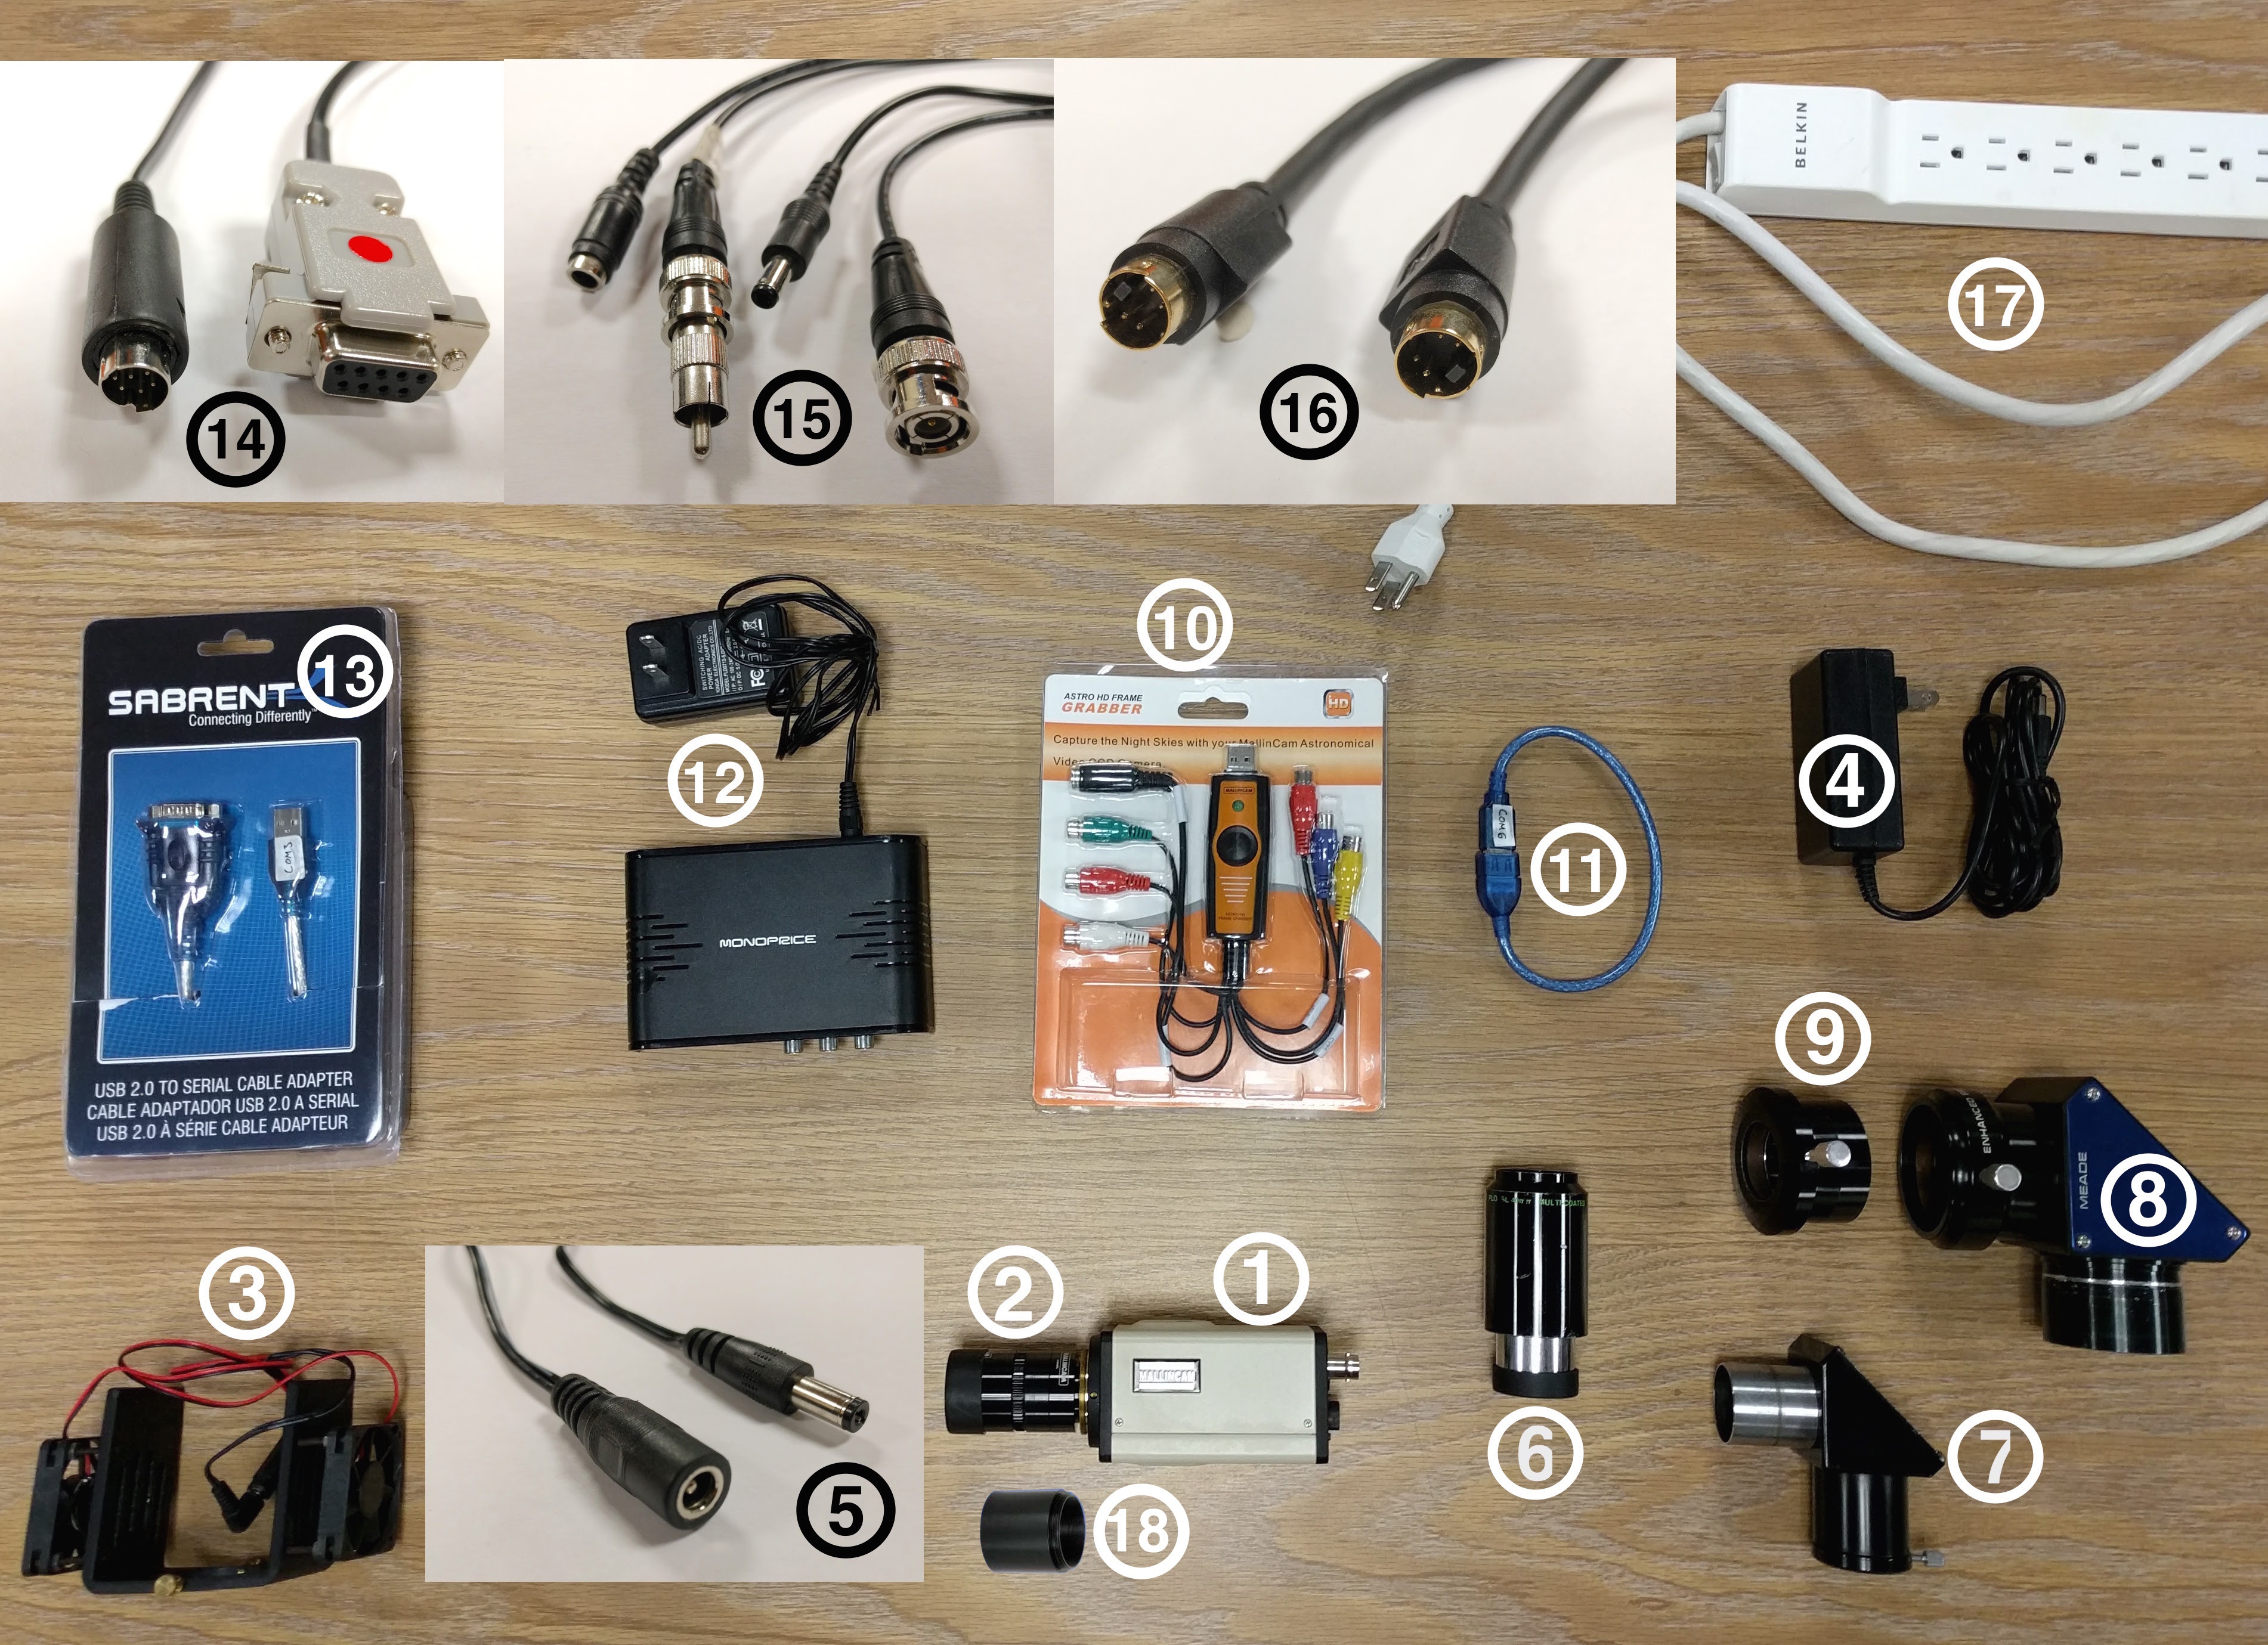
\includegraphics[width=.95\textwidth]{./images/MallinCam/astrofest_setup/equipment_numbered.jpg} 
	\end{center}
\end{figure}

\begin{enumerate}[label=\protect\circled{\arabic*}]
	\item MallinCam XII
	\item MFR-5 Mk II (0.33X) Focal Reducer (optional)
	\item Fan kit
	\item Fan kit power cable
	\item Fan kit power extension cable
	\item 40mm eyepiece
	\item 1.25'' star diagonal
	\item 2'' star diagonal
	\item 1.25'' eyepiece adapter
	\item Frame Grabber
	\item Frame Grabber extension cable
	\item Composite, S-Video, and HDMI to HDMI Converter
	\item USB 2.0 to serial cable adapter
	\item RS-232 serial computer-control cable (9-pin)
	\item Composite video cable
	\item 6' S-video cable
	\item Power strip
	\item 1.25'' eyepiece adapter (alternative to MFR-5 focal reducer)
	\item TV with analog video and HDMI inputs (not pictured)
	\item HDMI cable (not pictured)
	\item Laptop with Miloslick MallinCam control software (not pictured)\\
\end{enumerate}

\noindent The following procedure will prepare the MallinCam for observation by bringing a star into focus on the sensor. \\

\setcounter{rowcount}{0}
\begin{longtable}[t]{cc}

    \multicolumn{1}{m{.5\textwidth}}{\step Follow steps \ref{enum:quicksetup_start}-\ref{enum:quicksetup_end} of the Quick Setup Guide (Sec. \ref{ssec:betsy_quick}) to prepare the telescope for observation and bring a relatively bright star into focus with a 40mm eyepiece.\vspace{2em}
     
    \par \step Refer to Appendix \ref{sssec:focal_reduction} to to determine whether a focal reducer is necessary for your observation. If so, screw the MFR-5 focal reducer and optional spacer to the window of the MallinCam (pictured). Otherwise, screw in the 1.25`` eyepiece adapter.}
    & 
    \raisebox{-.5\totalheight}{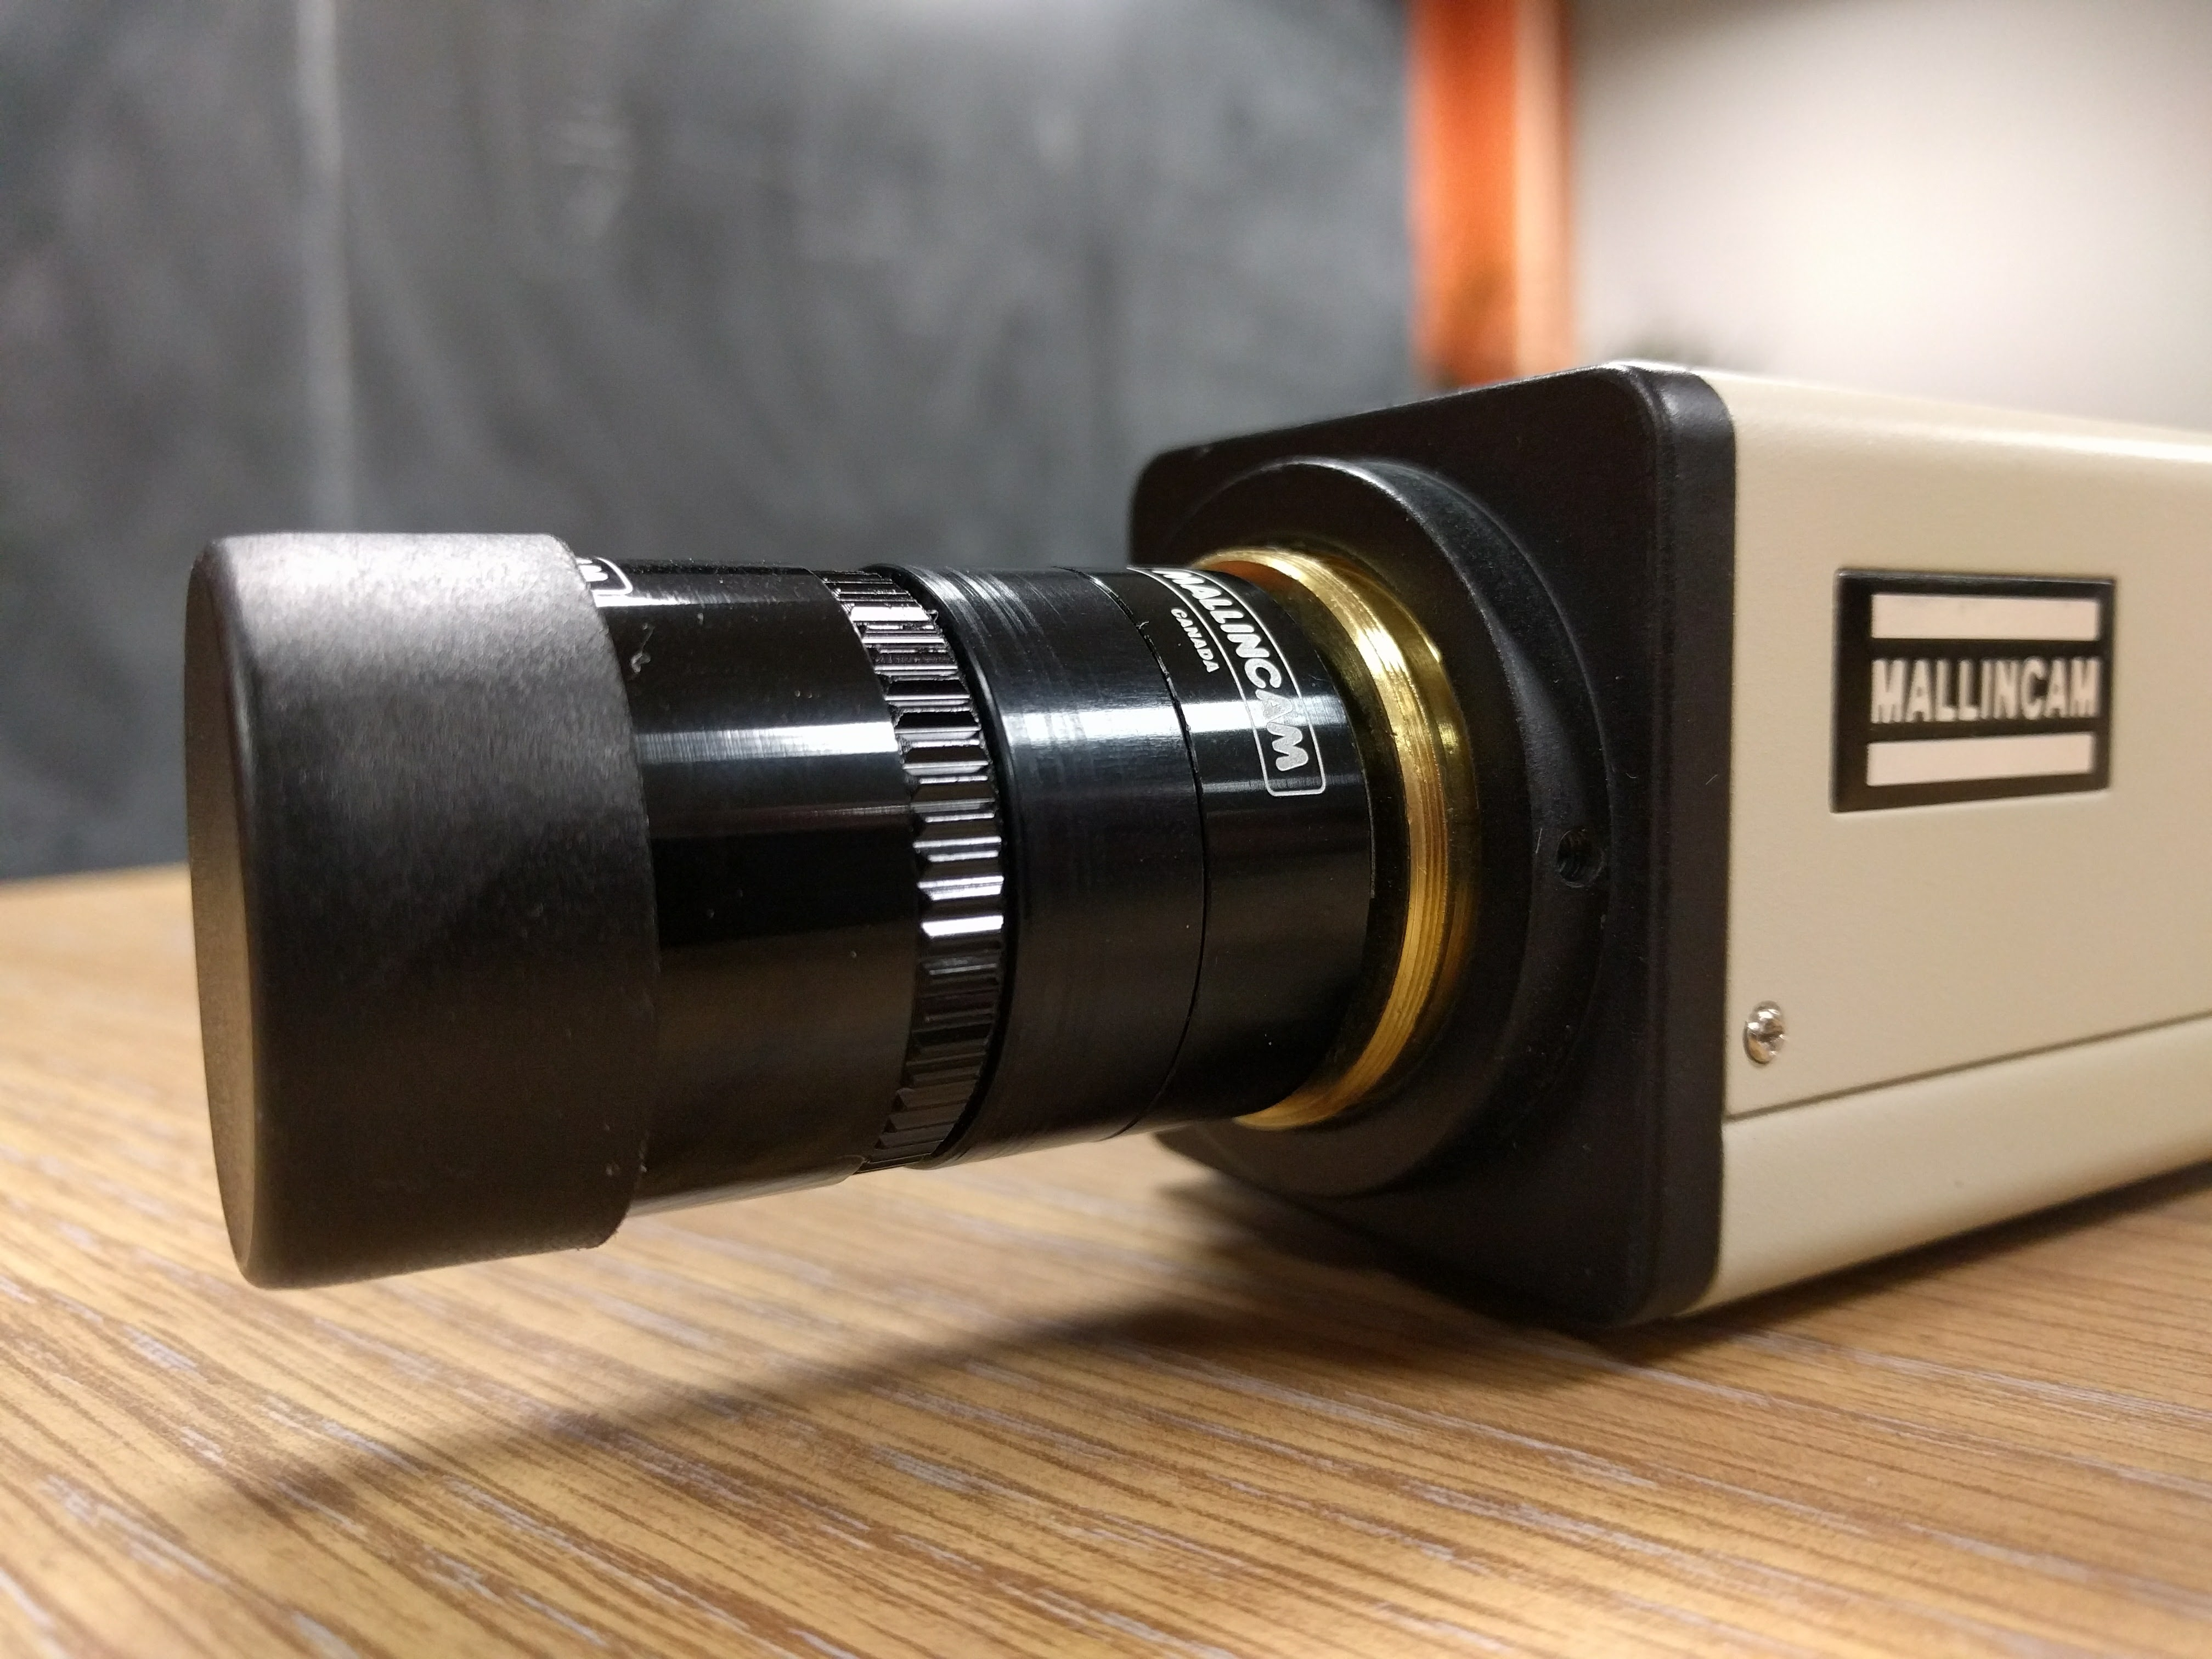
\includegraphics[width=.5\textwidth]{./images/MallinCam/astrofest_setup/focal_reducer.jpg}} \\[8em]
    
    \multicolumn{1}{m{.5\textwidth}}{\step Attach the fan kit to the MallinCam by tightening the two screws on the top and bottom of kit into threads above and below MallinCam window. Plug the fan kit into the MallinCam power input.} 
    & 
    \raisebox{-.5\totalheight}{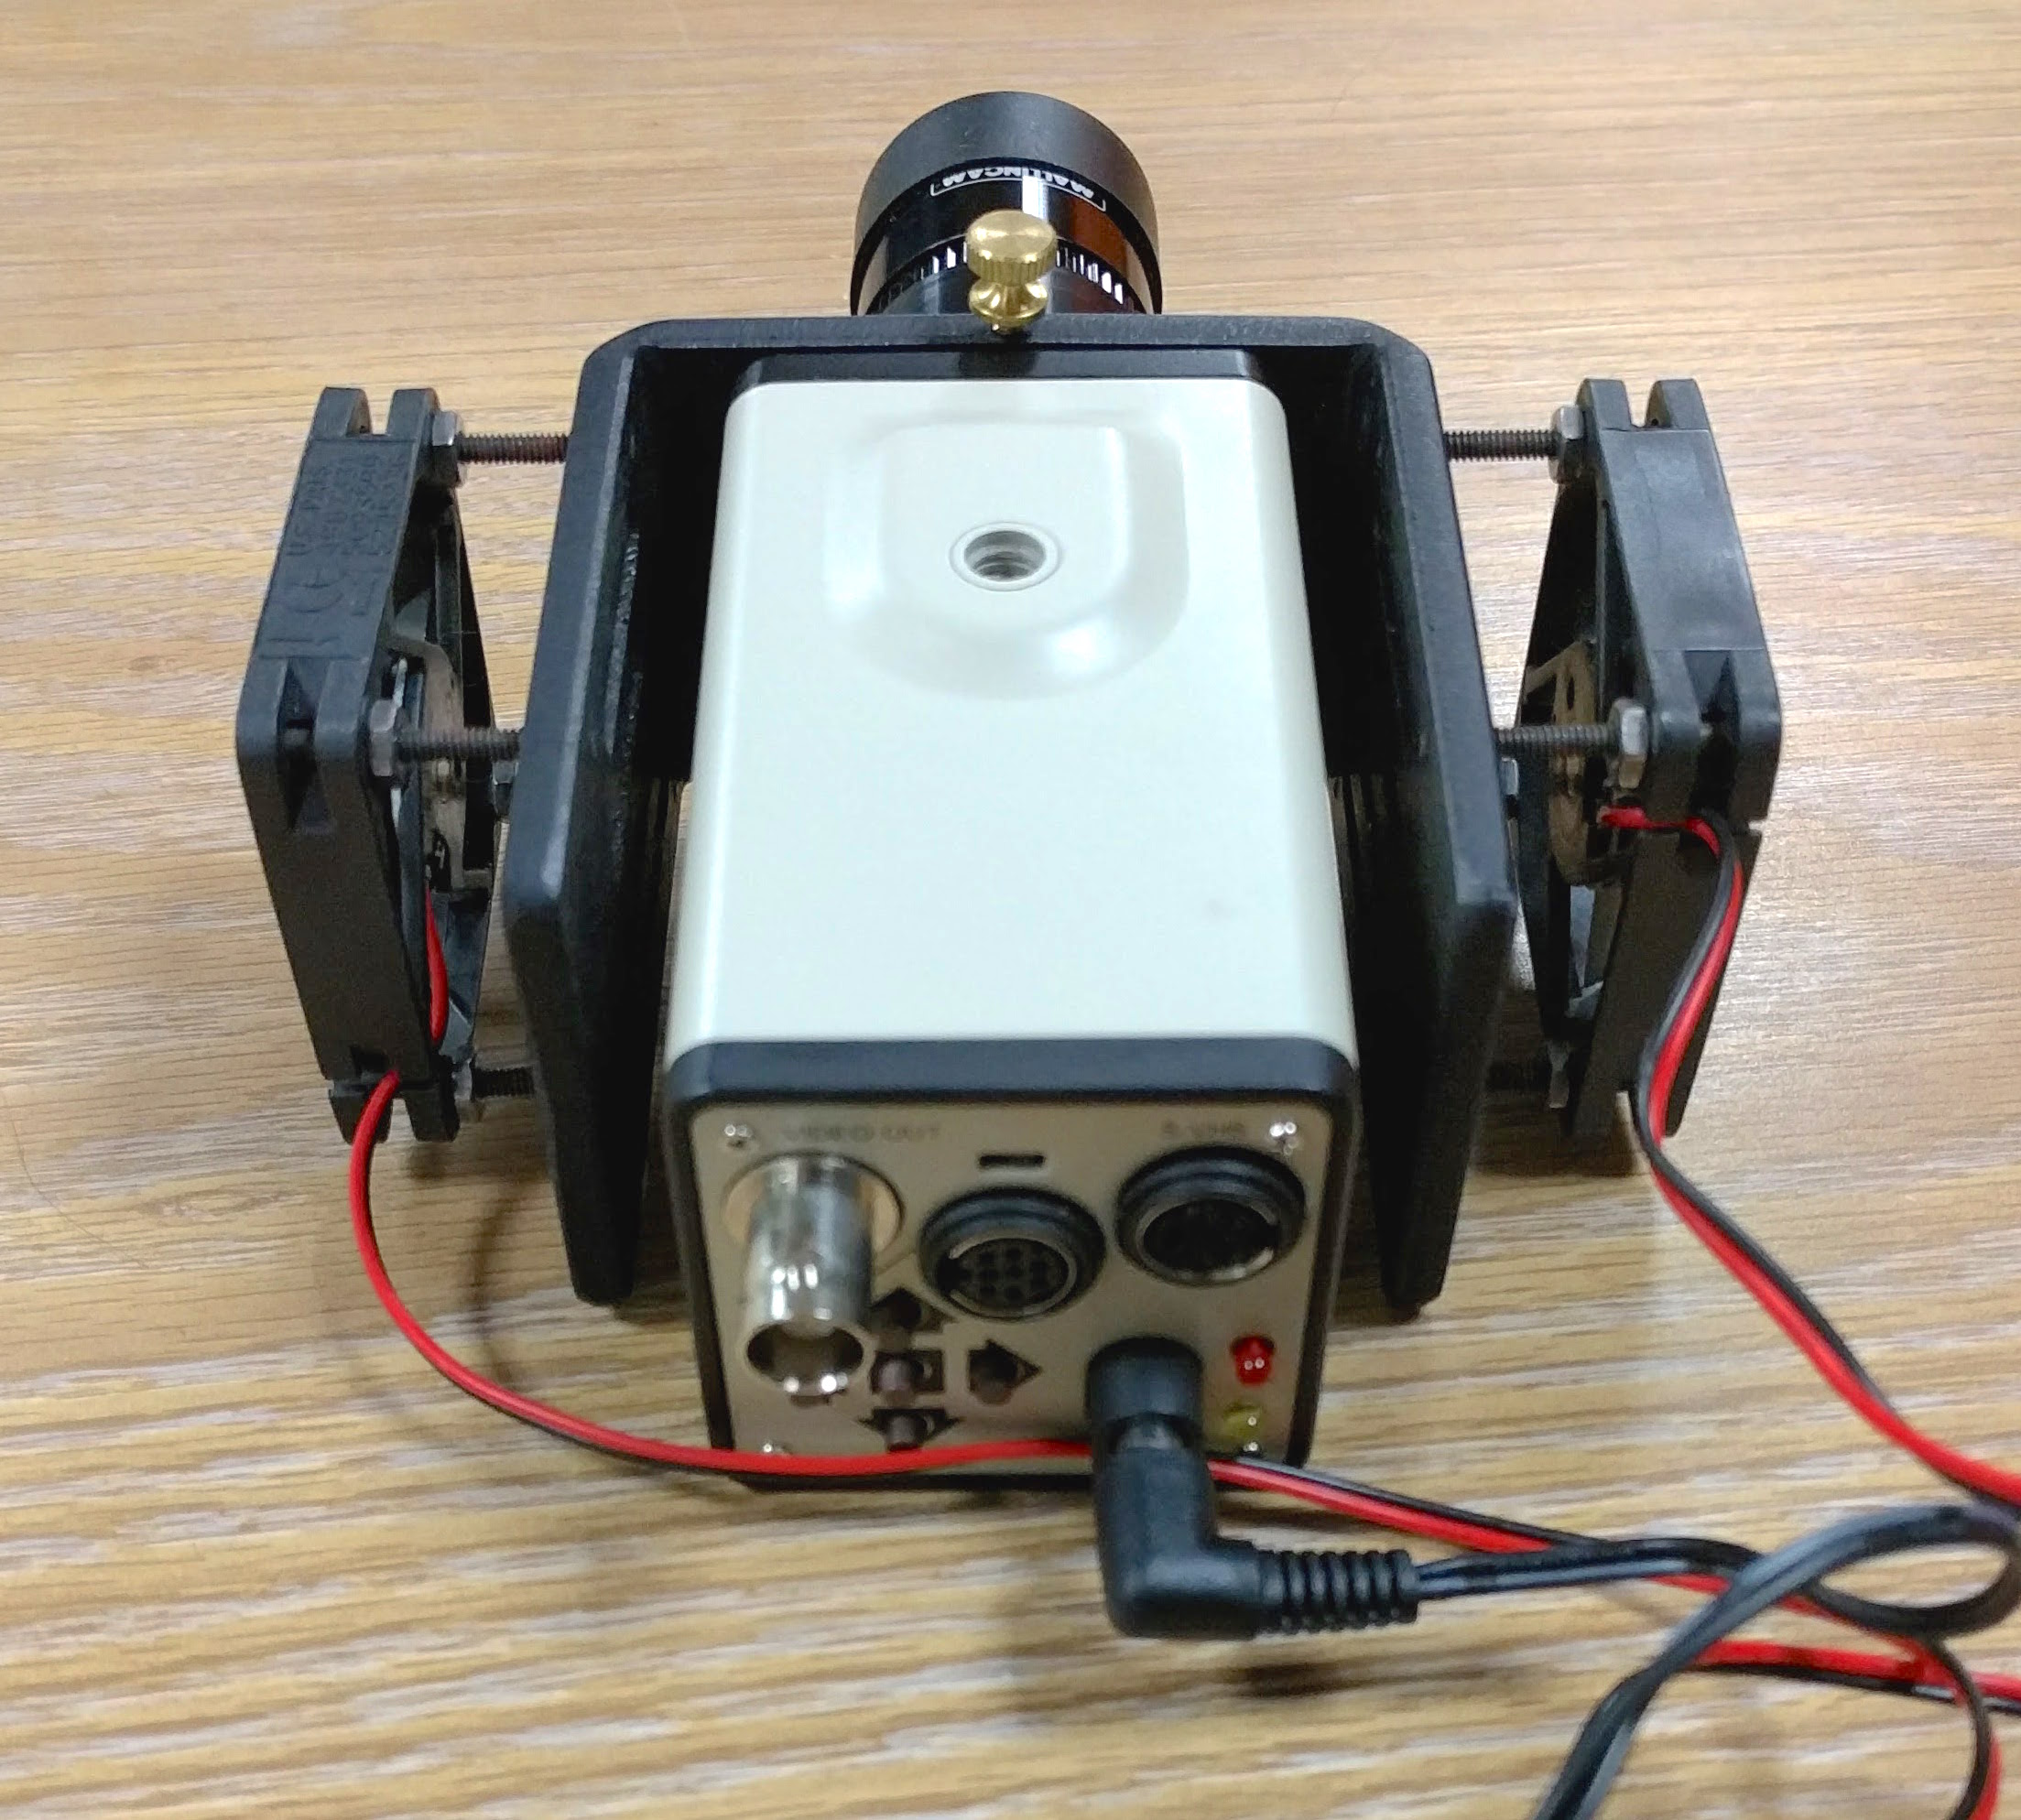
\includegraphics[width=.5\textwidth]{./images/MallinCam/astrofest_setup/fankit.jpg}} \\[8em]
    
    \multicolumn{1}{m{.5\textwidth}}{\step Connect the fan kit power extension cable to the fan kit power cable and the extension cable to the fan kit input. Plug the power cable into the power strip. Plug the power strip in at the base of the telescope. Turn the power strip on. The red power indicator light on the MallinCam and the fan kit should both turn on.} 
    & 
    \raisebox{-.5\totalheight}{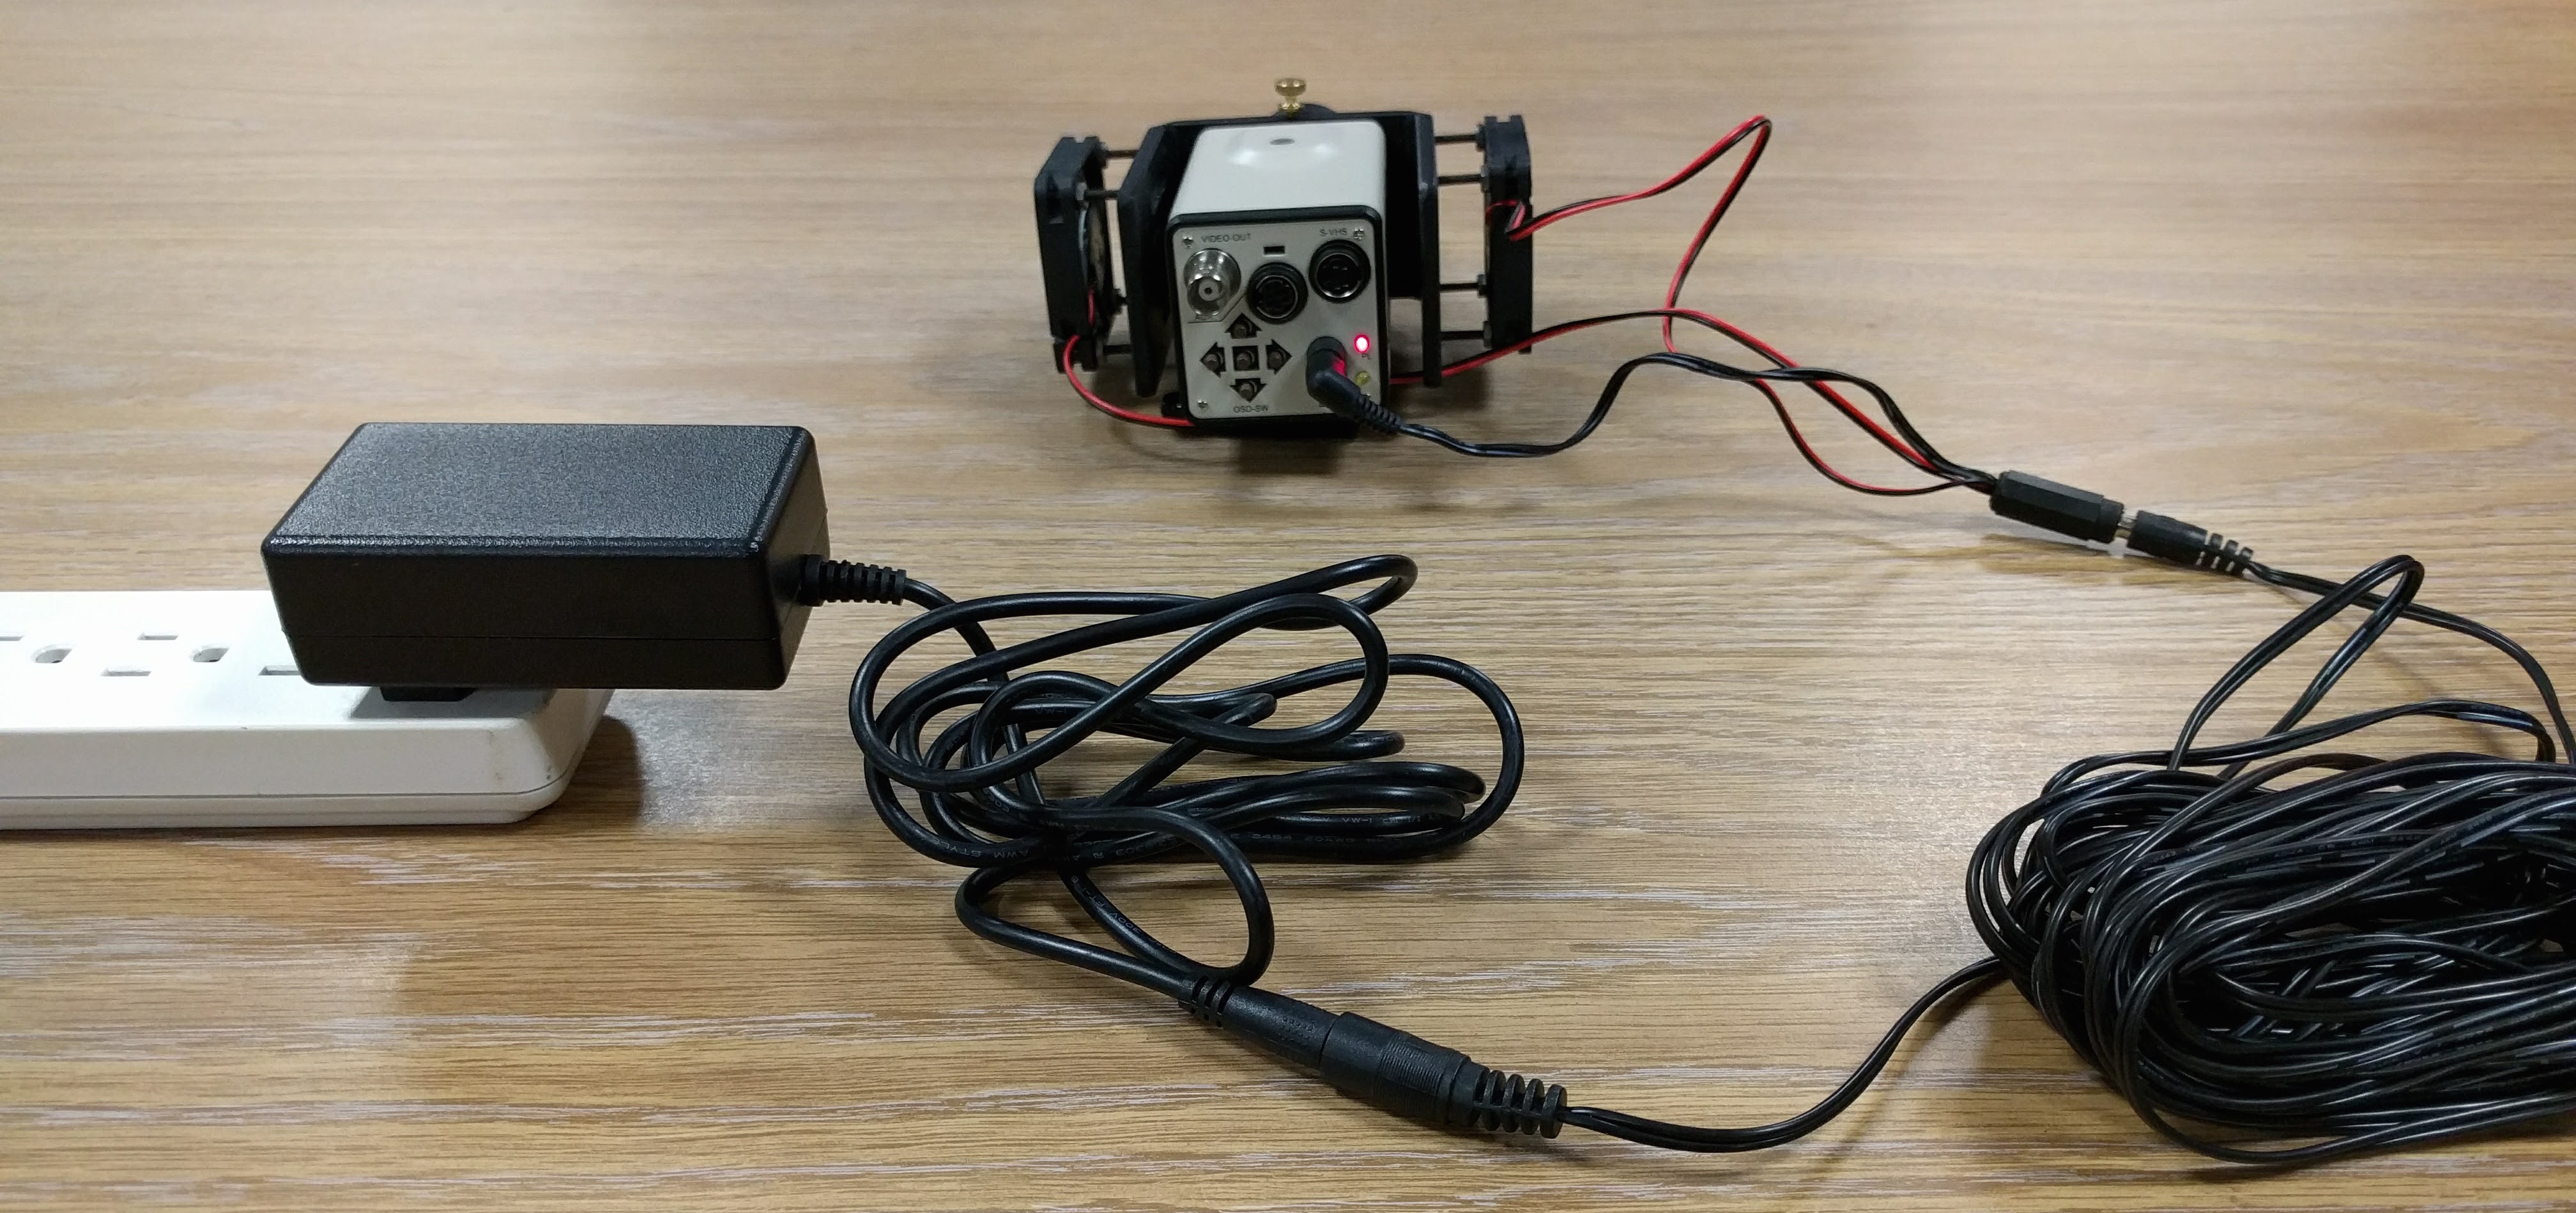
\includegraphics[width=.5\textwidth]{./images/MallinCam/astrofest_setup/power_on.jpg}} \\[8em]       
    
    \multicolumn{1}{m{.5\textwidth}}{\step Launch Miloslick MallinCam Control software from the laptop. \vspace{2em} 
    \par \step Connect the RS-232 control cable to the USB adapter. Tighten screws.} 
    & 
    \raisebox{-.5\totalheight}{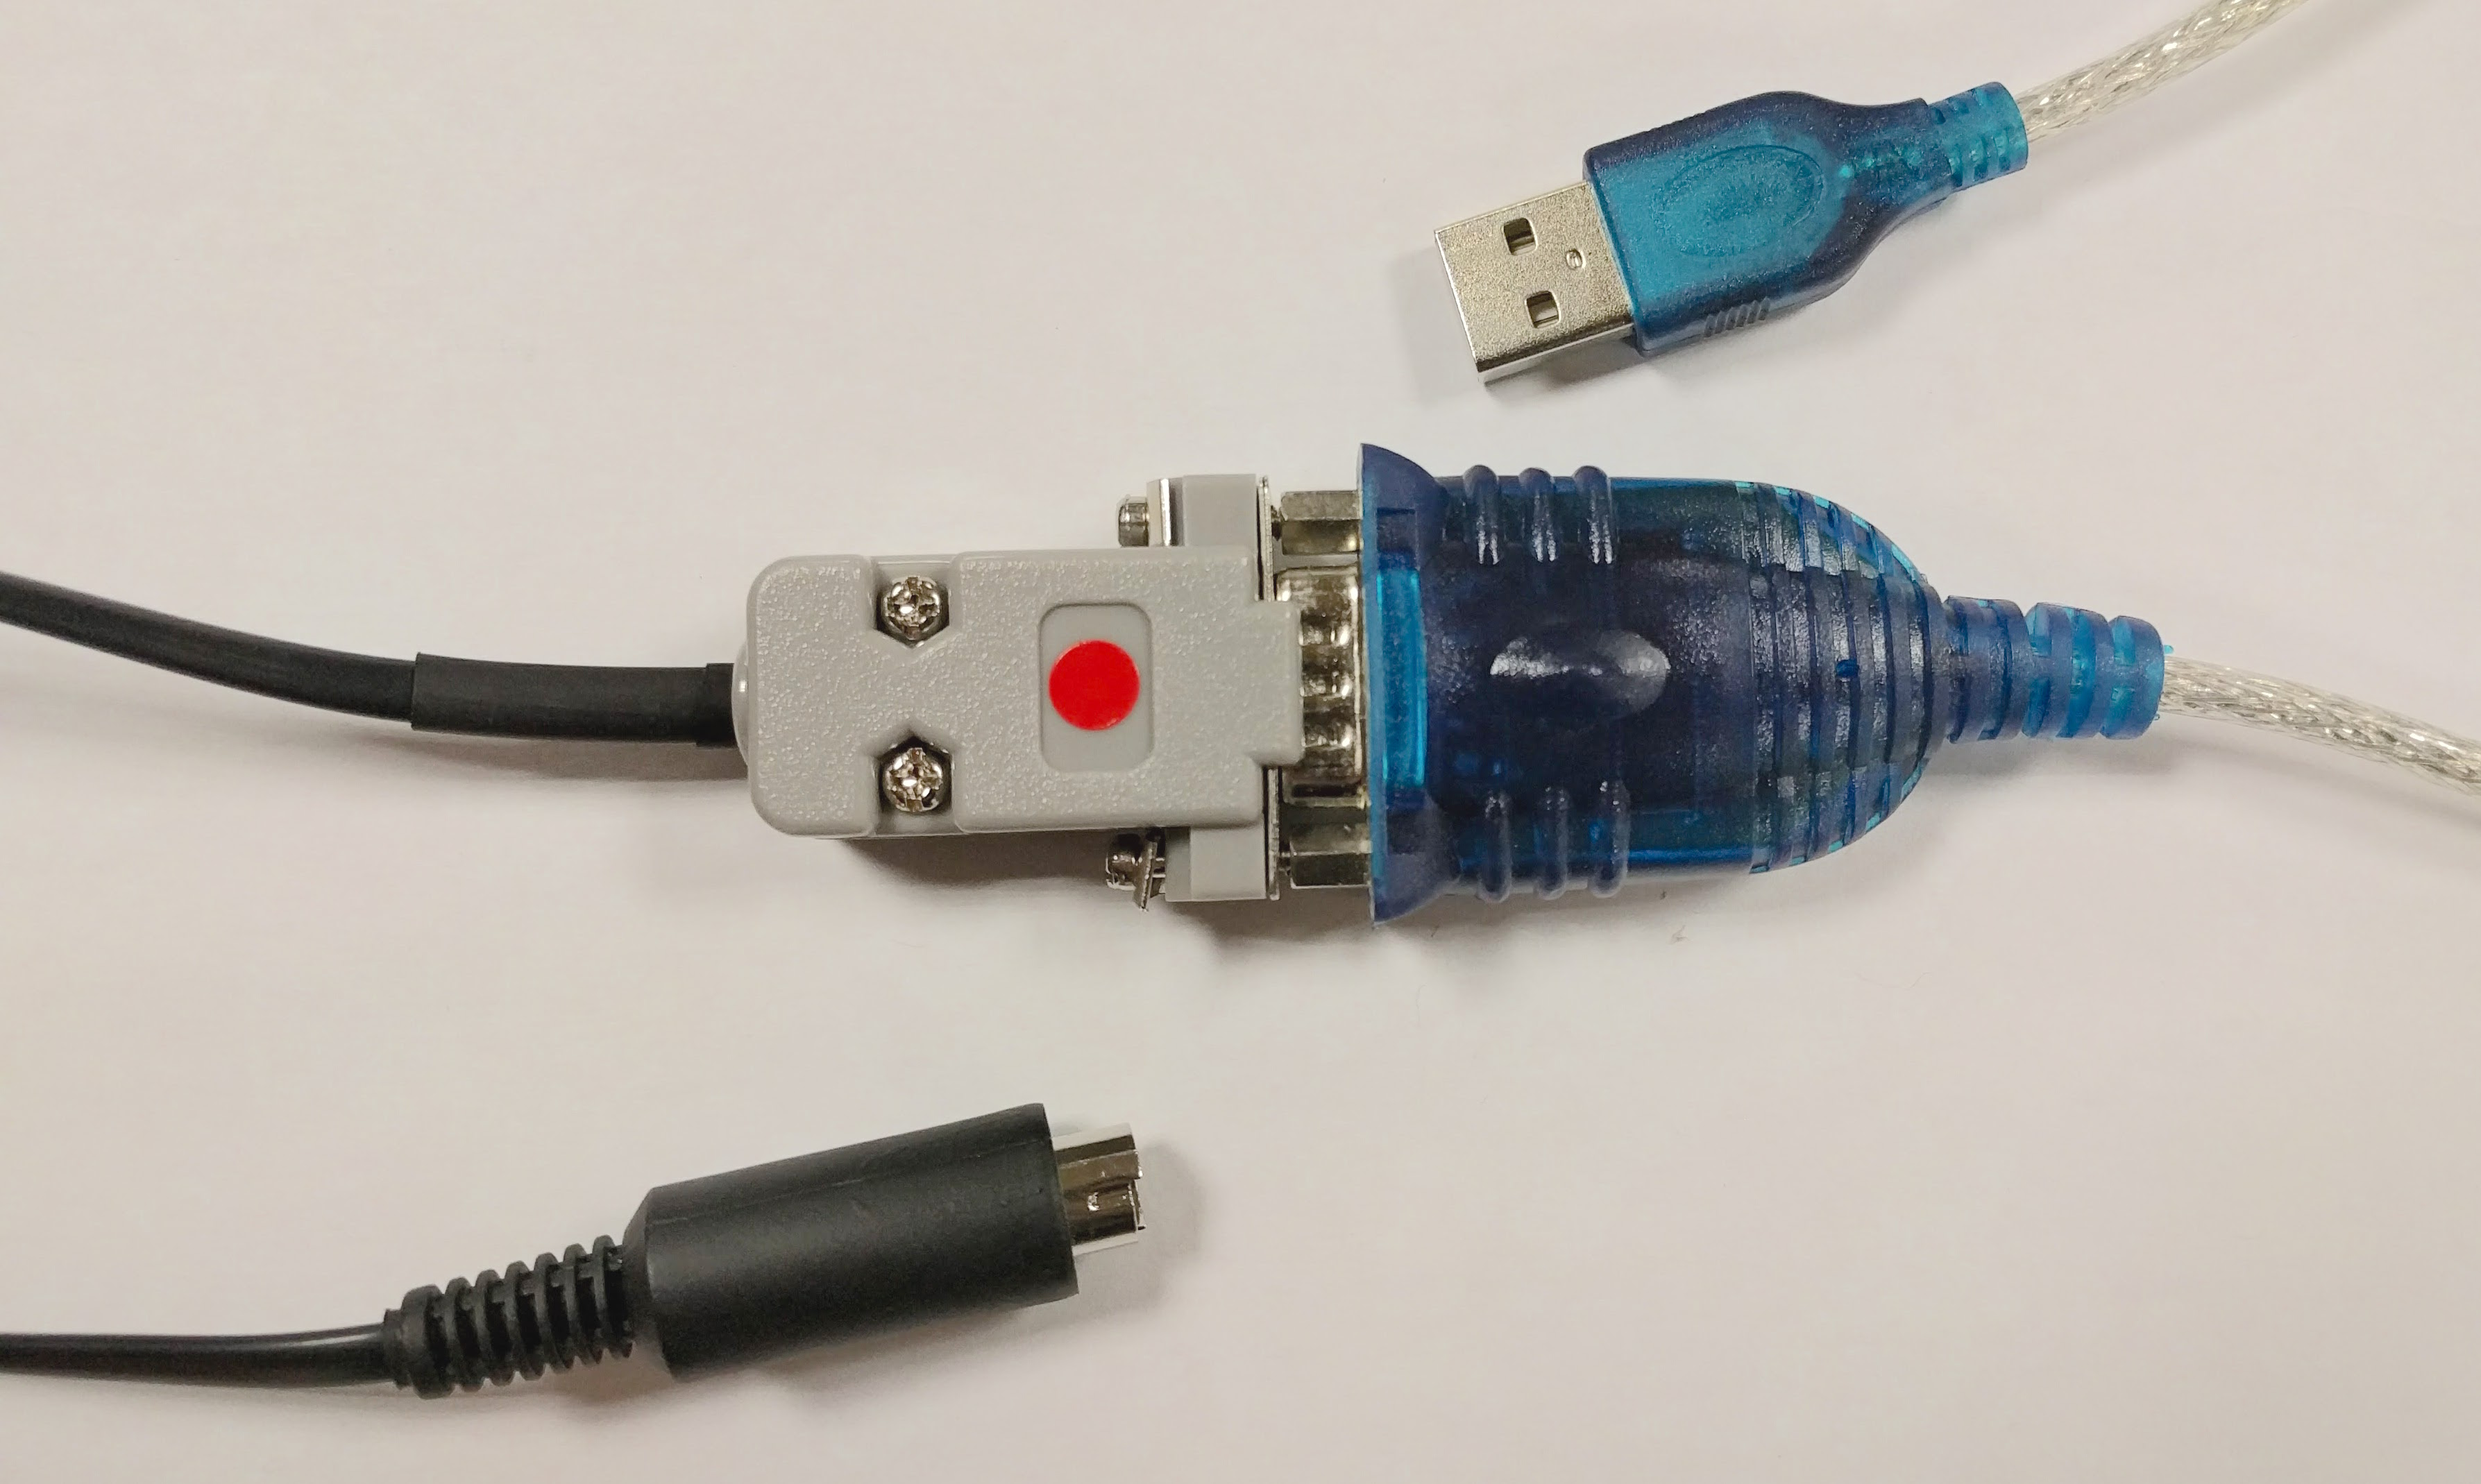
\includegraphics[width=.5\textwidth]{./images/MallinCam/astrofest_setup/rs232-usb.jpg}}\\[8em]
    
    \multicolumn{1}{m{.5\textwidth}}{\step Connect the other end of the RS-232 control cable to the computer control port on the MallinCam and plug the USB end of the adapter into the computer.
    You may get a notification from Miloslick to "reset camera settings to default values". Click OK.
    The bottom-left corner of the Miloslick window should read "MCXtreme X2/PC: Connected". See Sec. \ref{ssec:x2troubleshoot} troubleshooting.}
    & 
    \raisebox{-.5\totalheight}{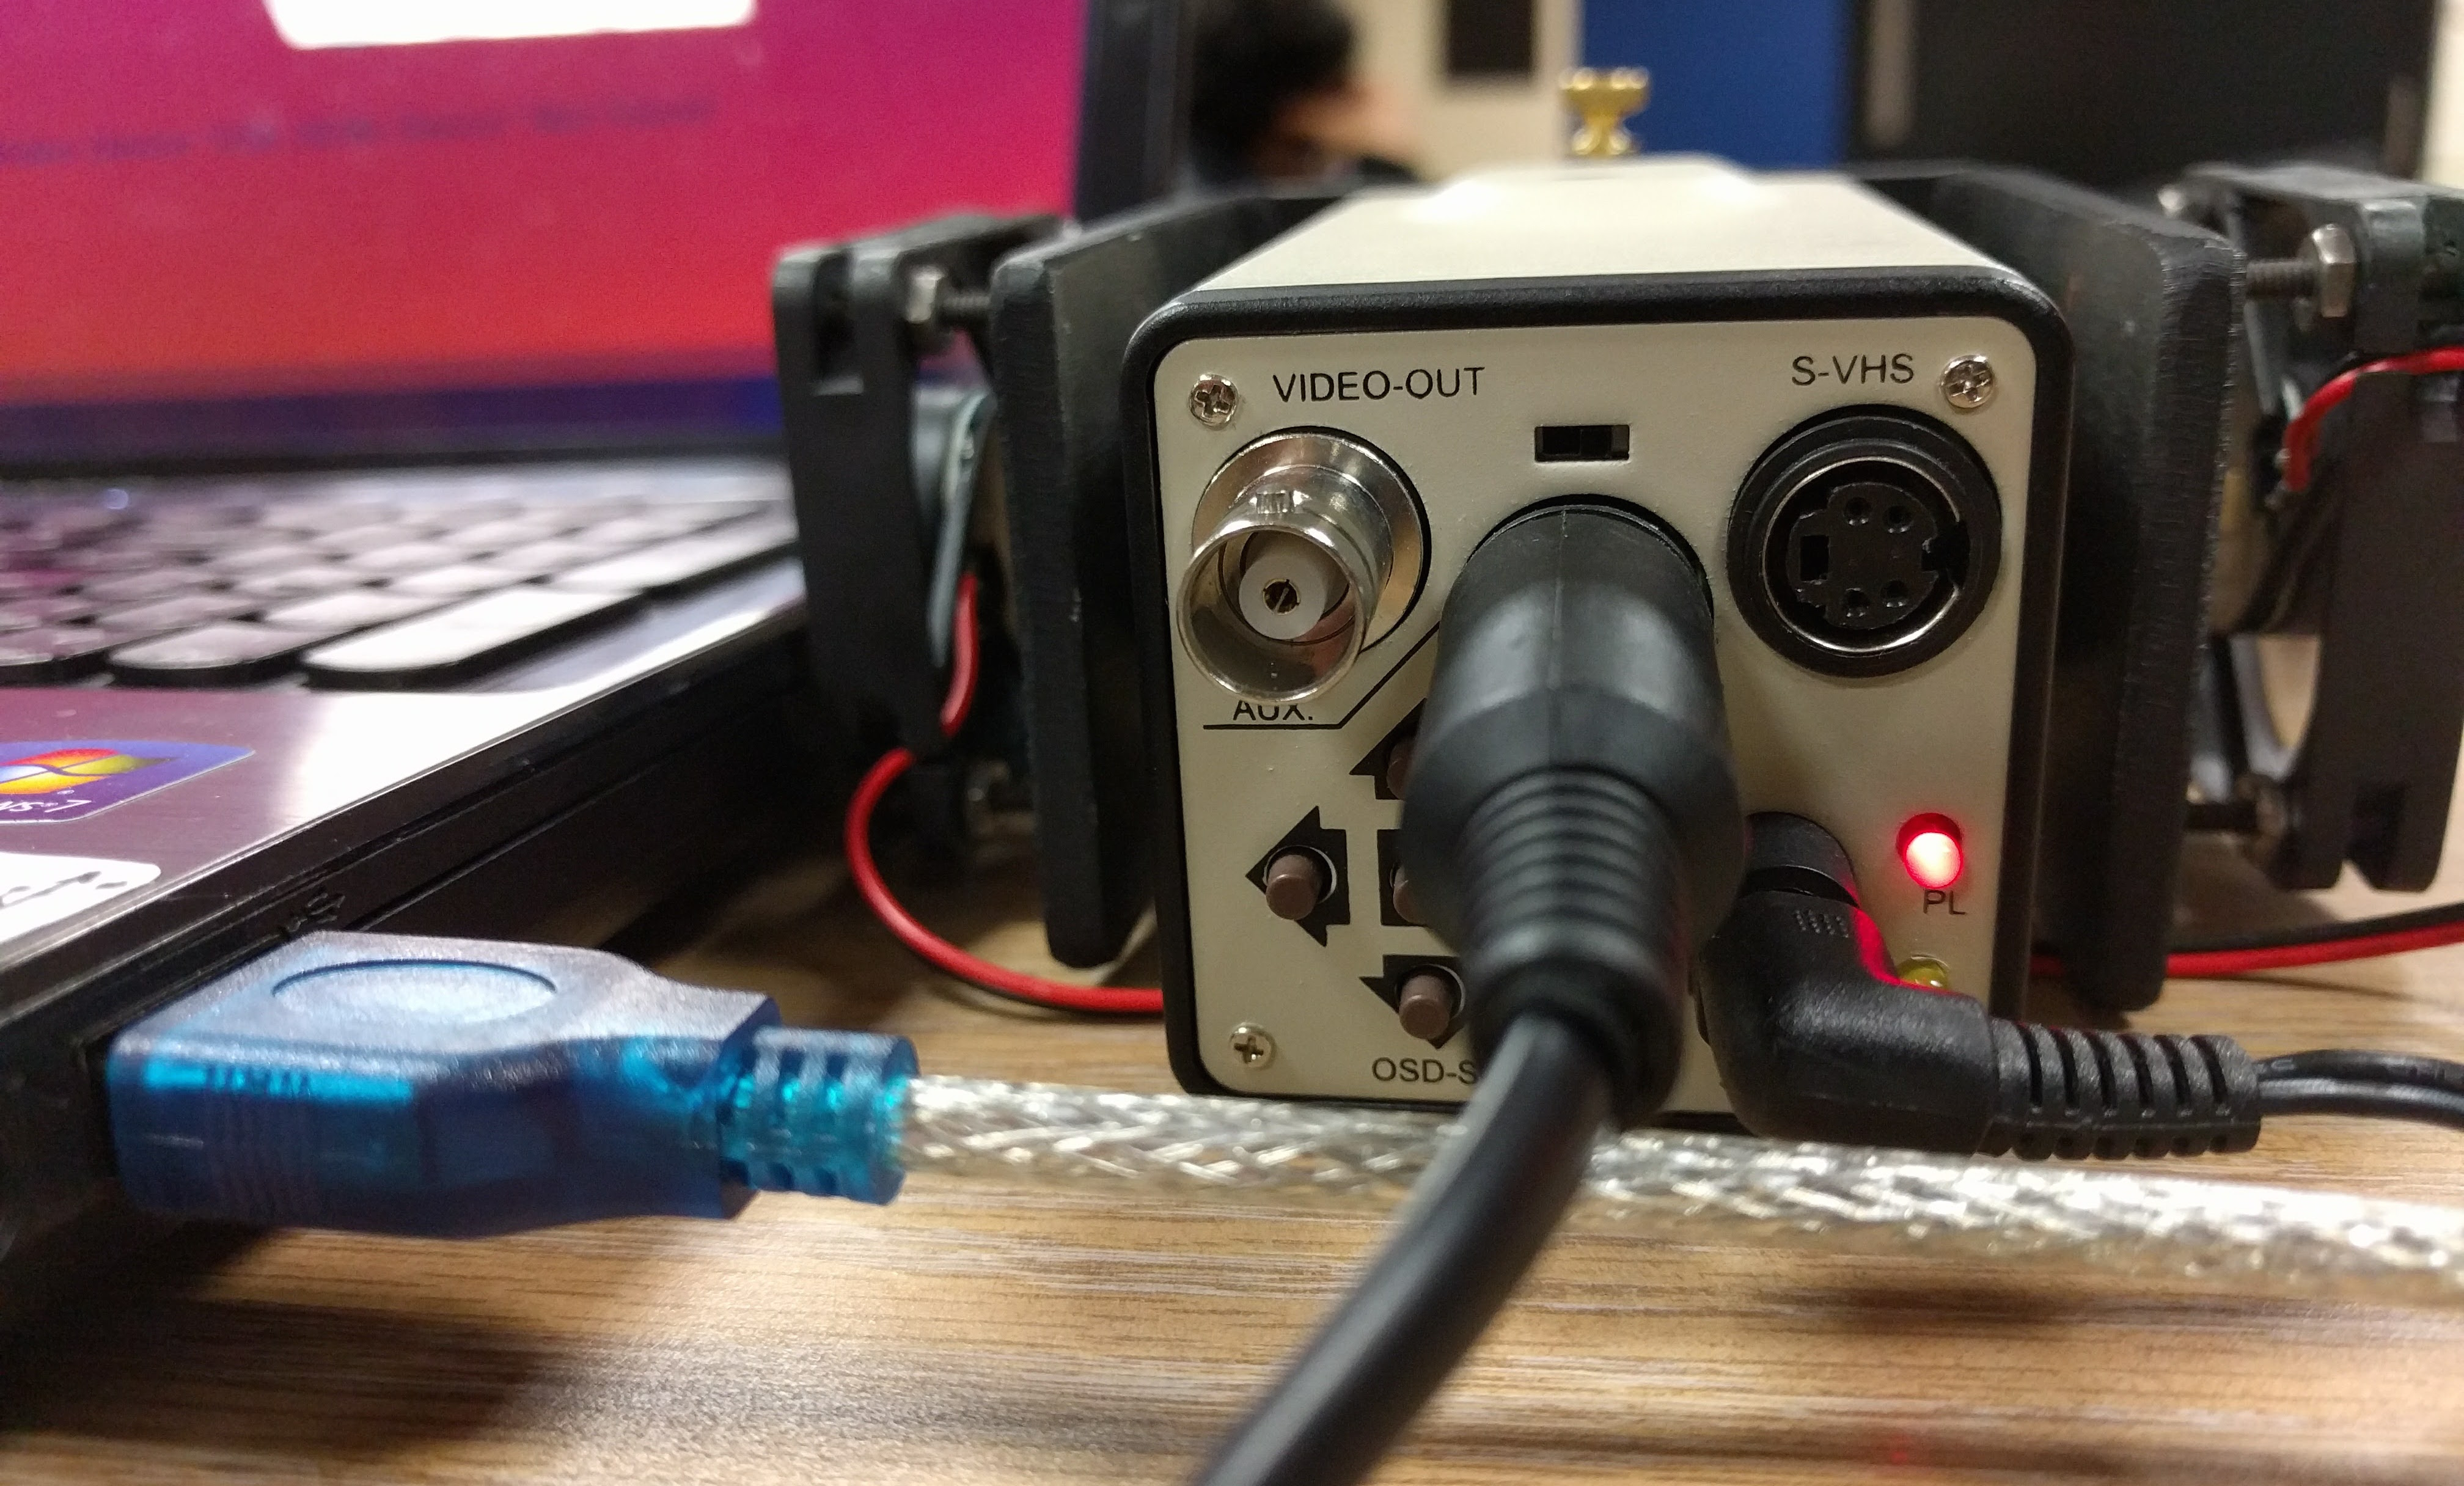
\includegraphics[width=.5\textwidth]{./images/MallinCam/astrofest_setup/computer_connect.jpg}} \\[8em]
    
    \multicolumn{1}{m{.5\textwidth}}{\step Plug the male end of the frame grabber extension cable into the USB port on the other side of the laptop. Plug the frame grabber into the female end of the extension cable.} 
    & 
    \raisebox{-.5\totalheight}{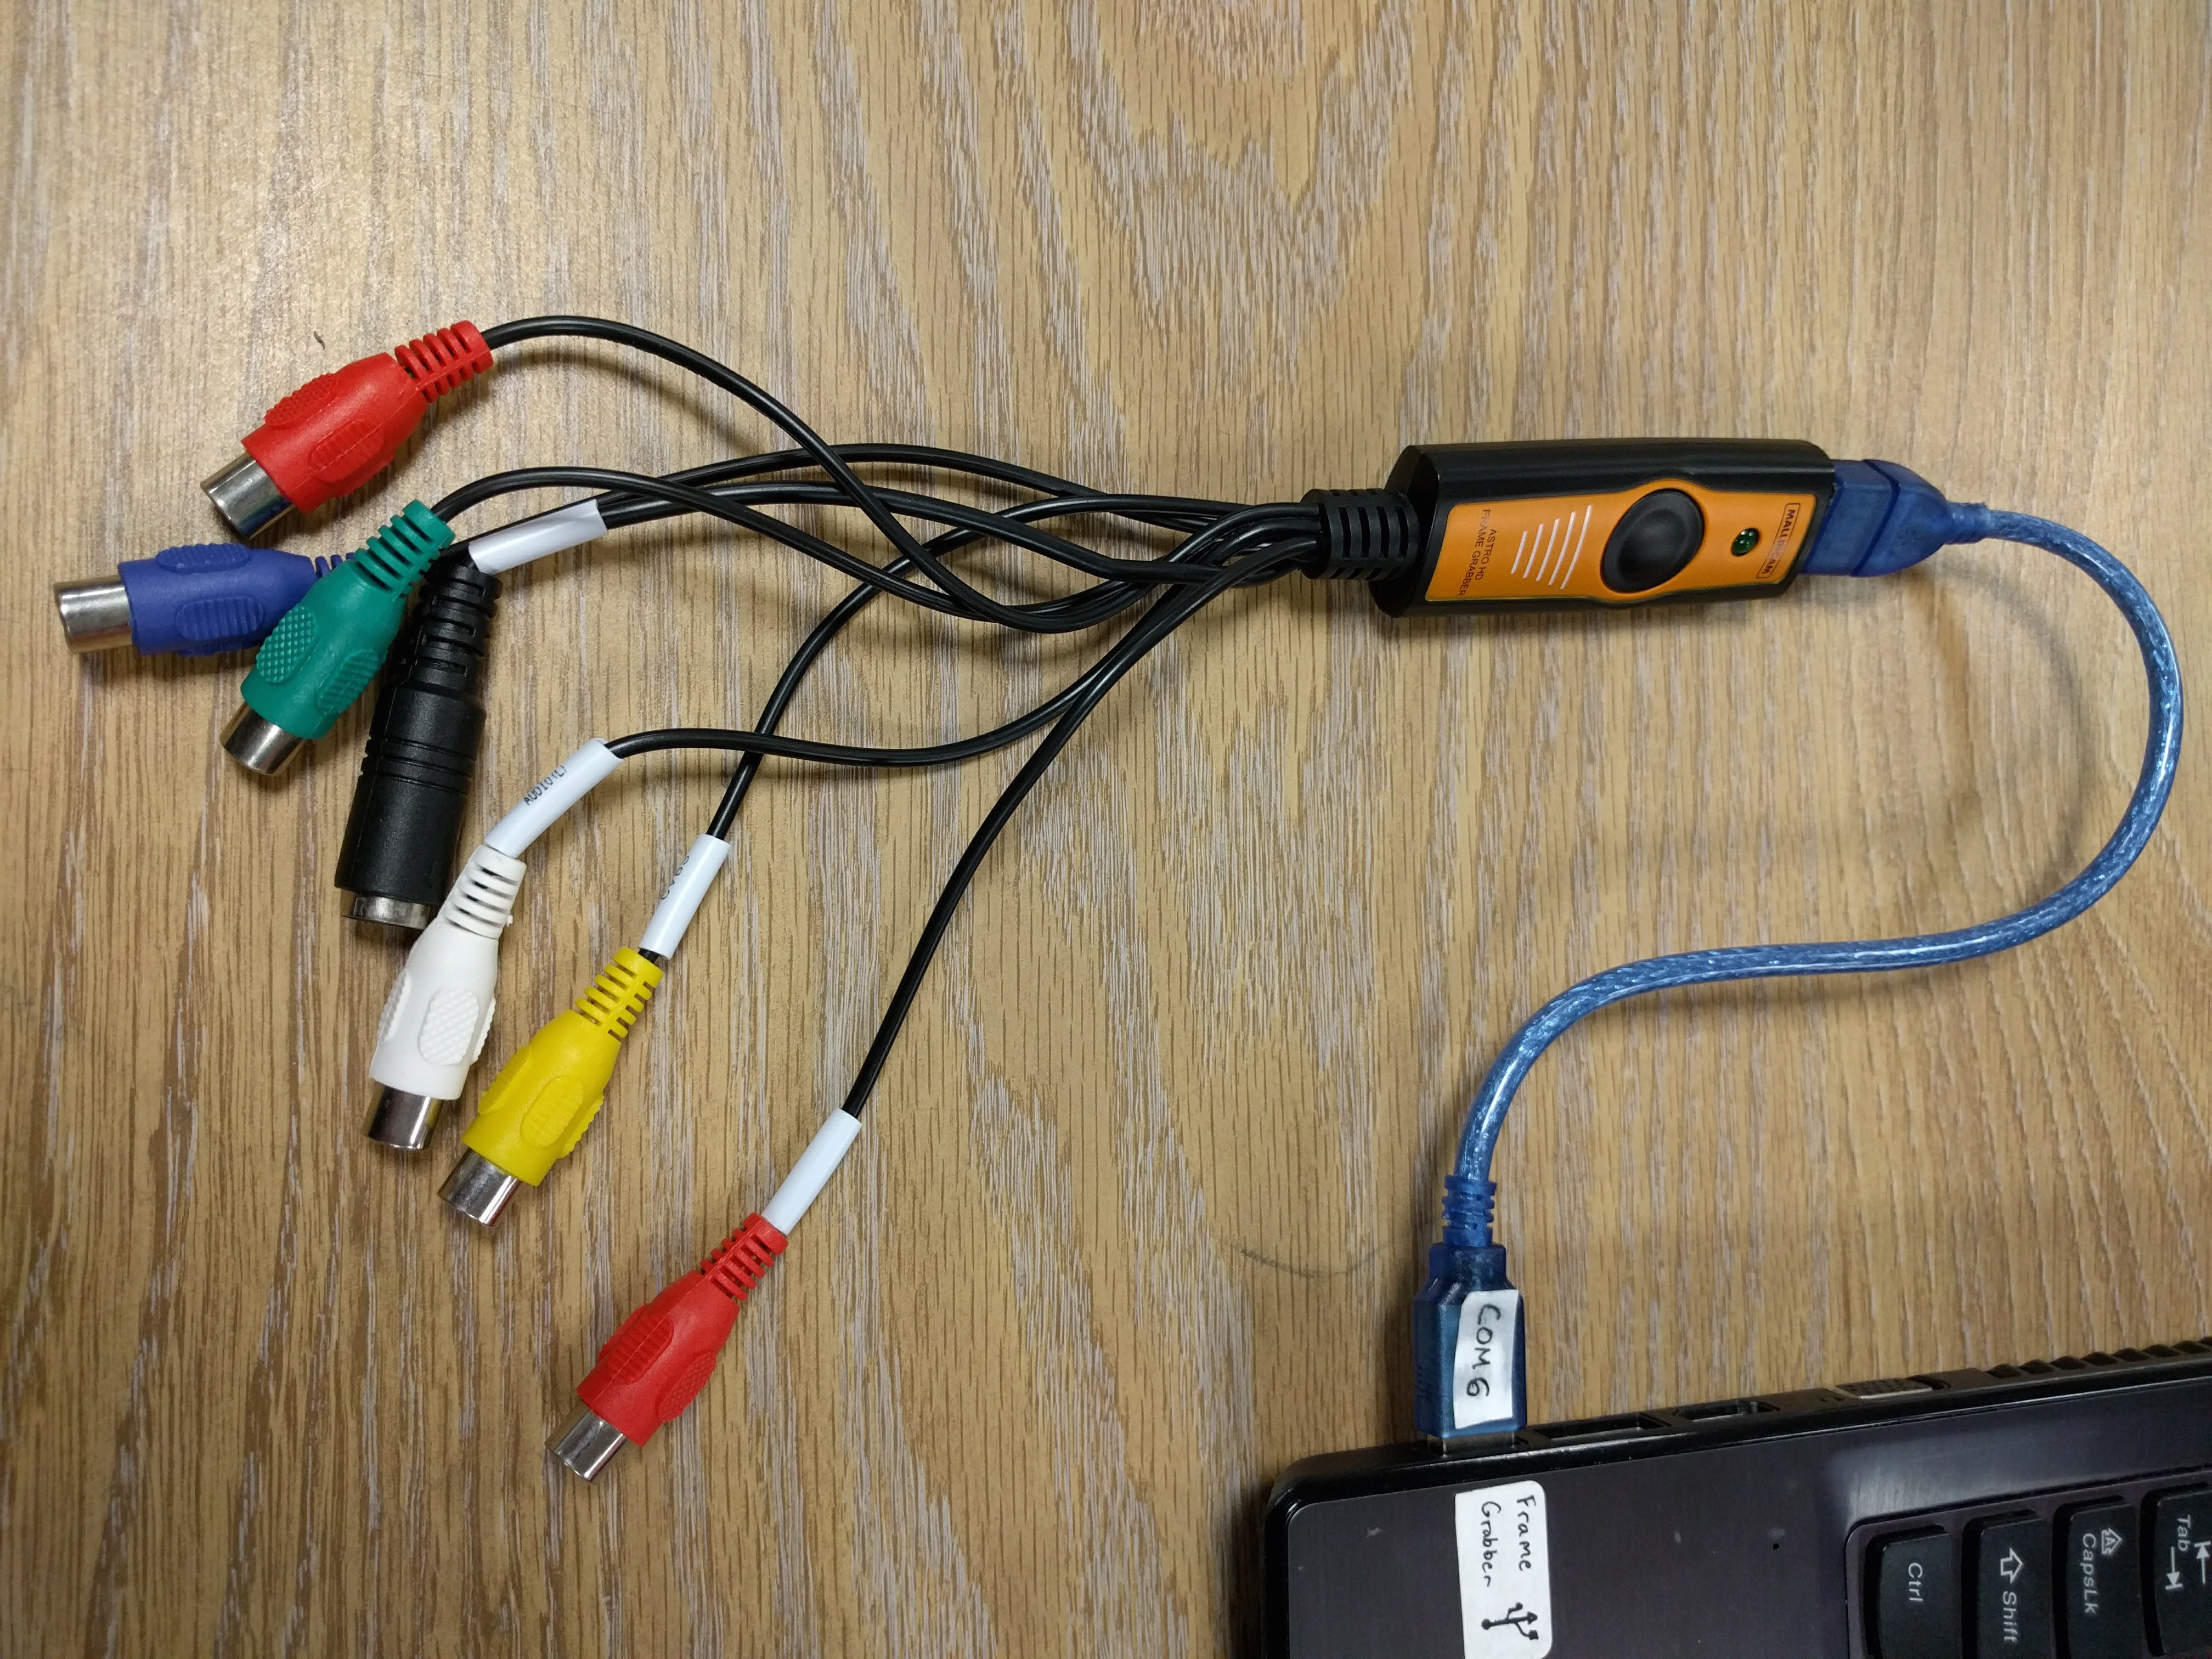
\includegraphics[width=.5\textwidth]{./images/MallinCam/astrofest_setup/frame_grabber.jpg}} \\[8em] 
    
    \multicolumn{1}{m{.5\textwidth}}{\step Plug the female end of the composite video cable into the video-out (BNC) input on the MallinCam. Twist the ring on the cable lock the cable in place. Plug the male end (RCA) of the composite video cable into the video RCA input (yellow) on the frame grabber.} 
    & 
    \raisebox{-.5\totalheight}{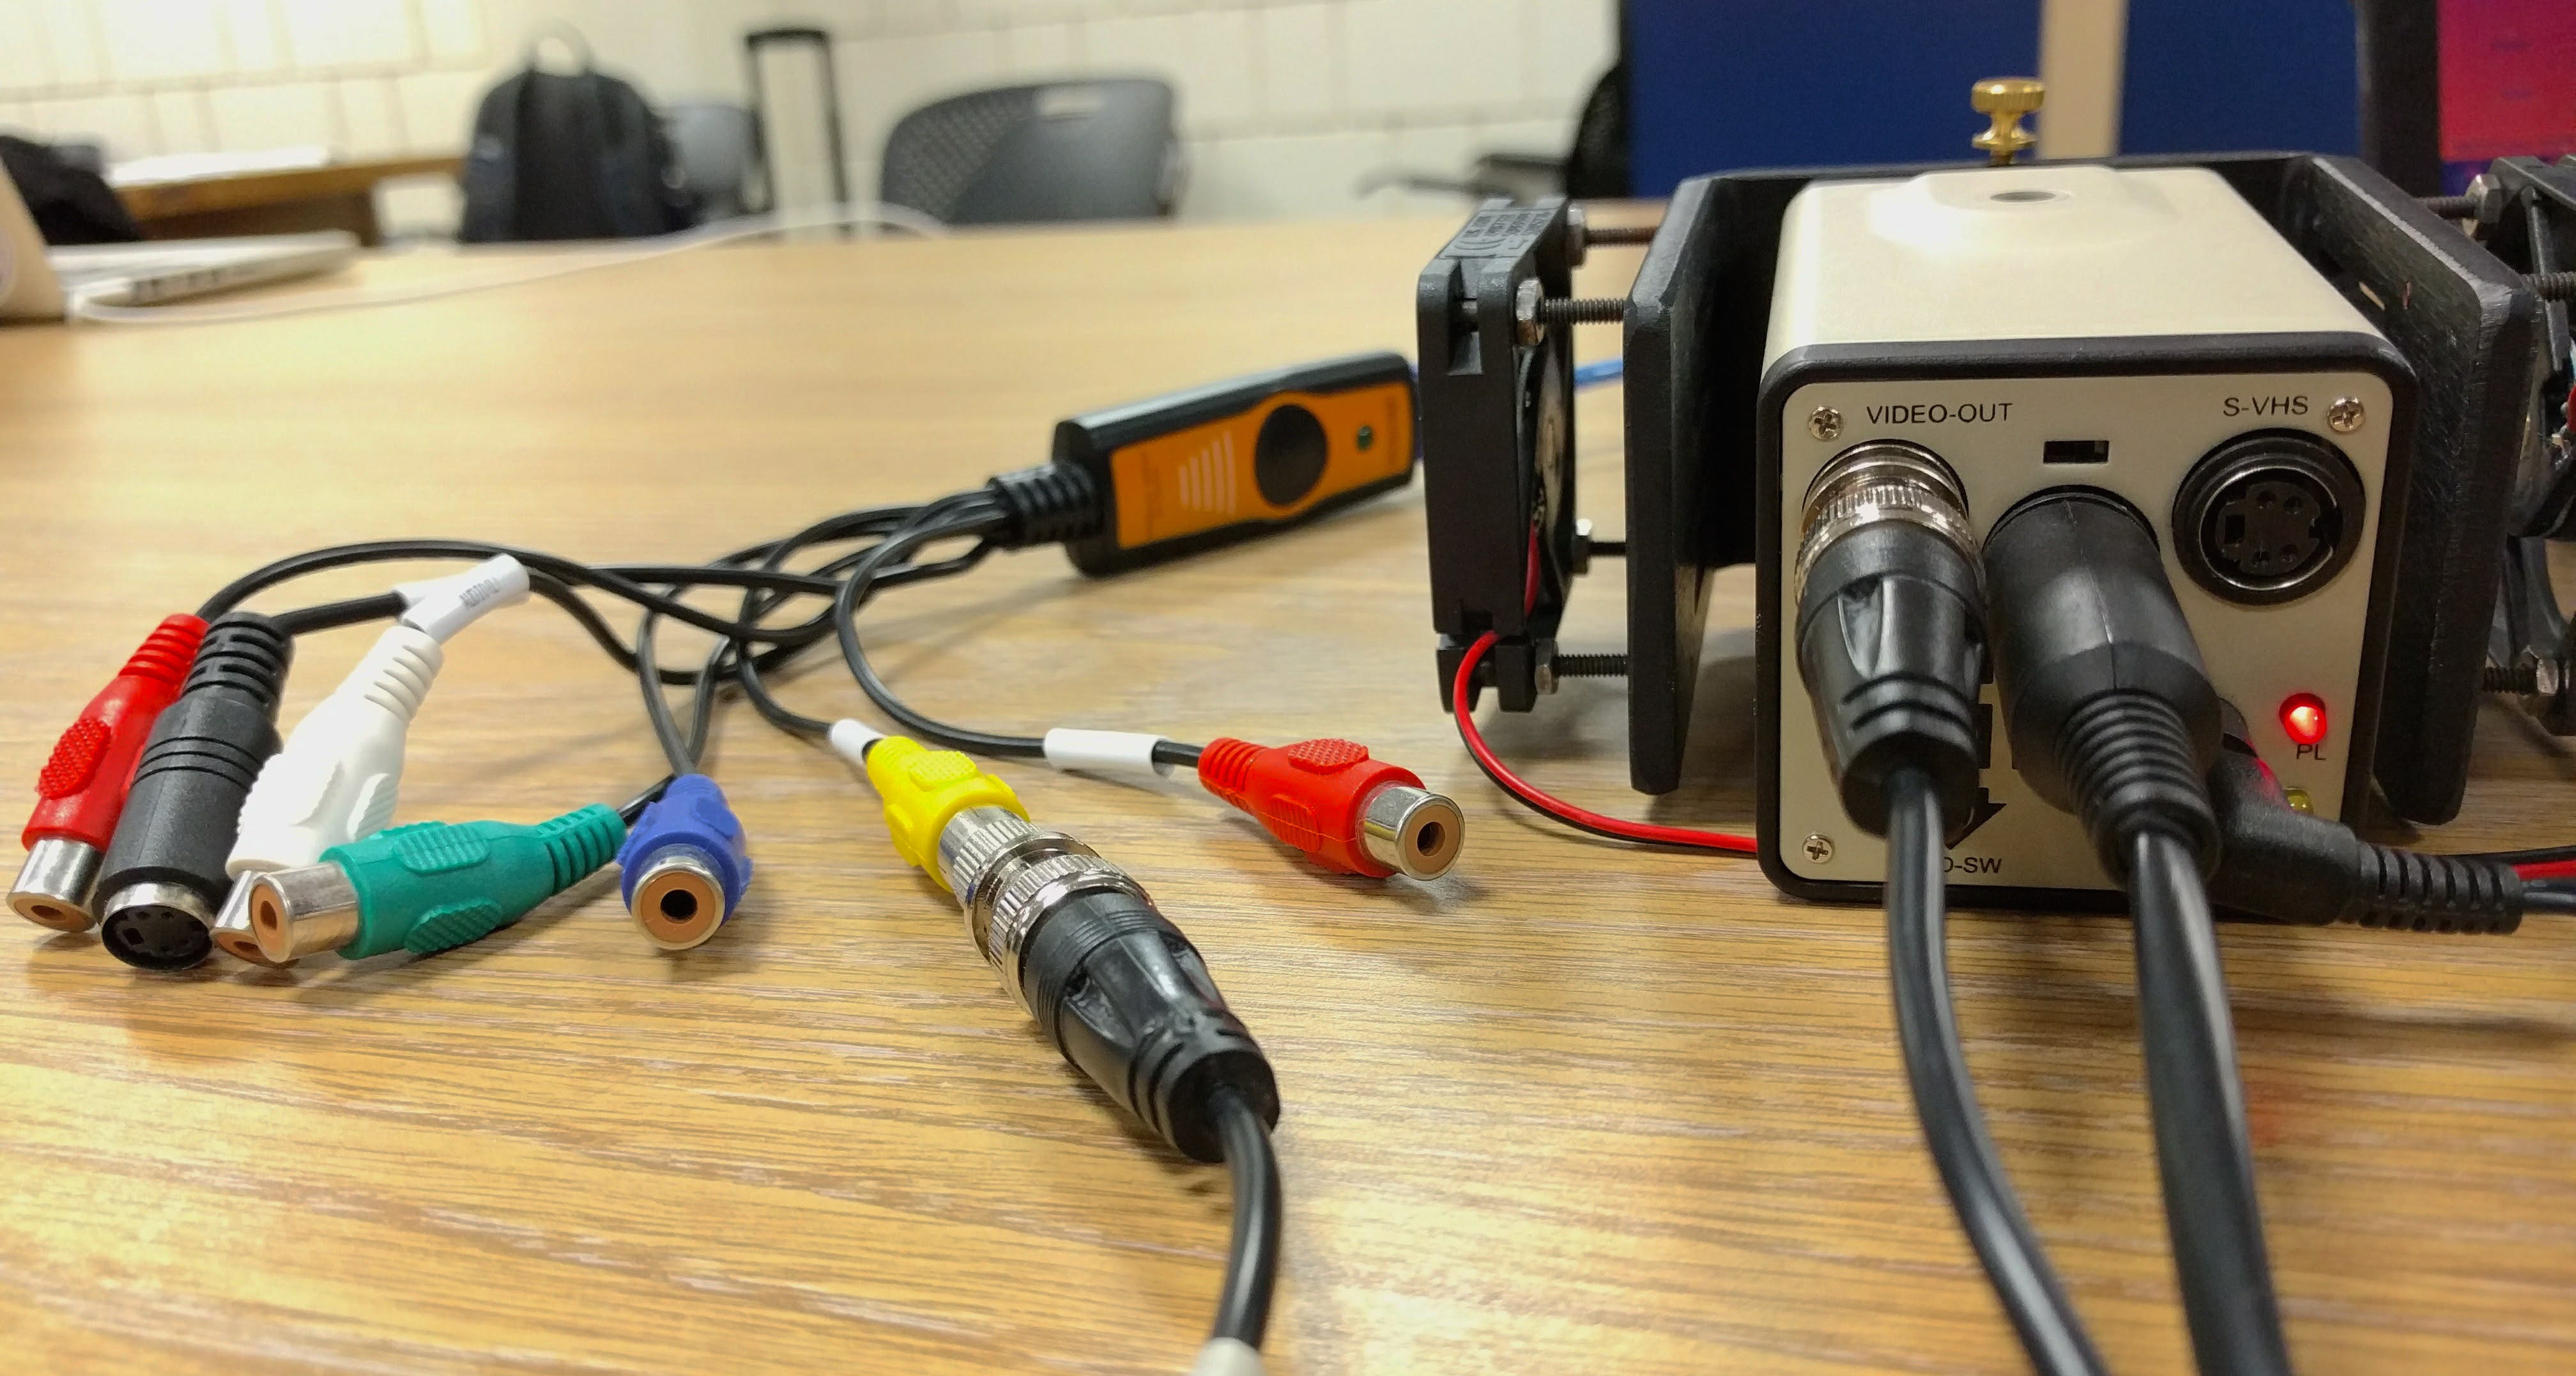
\includegraphics[width=.5\textwidth]{./images/MallinCam/astrofest_setup/frame_grabber_connect.jpg}}
\end{longtable}
\begin{longtable}{c}    
    \multicolumn{1}{m{\textwidth}}{\step In Miloslick, from the top menu bar click Video $>$ Video Device $>$ USB 2828x Device. The green light on the frame grabber should turn on and the video feed should be displayed in Miloslick. If the USB 2828x Device is not listed in Video Devices, try unplugging and re-plugging the frame grabber. See Sec. \ref{ssec:x2troubleshoot} for troubleshooting.}\\[4em]
    
    \multicolumn{1}{m{\textwidth}}{\step To simultaneously test the composite video connection and computer connection to the camera, scroll to the bottom of the Camera Settings pane on the left side of Miloslick and check the color bars box. If color bars appear in the video feed, the computer and composite video connections have been established correctly.}
\end{longtable}
\begin{longtable}[t]{cc}

	\multicolumn{1}{m{.5\textwidth}}{\step Plug the HDMI cable into the HDMI output of the HDMI converter box. Plug the converter box power cable into the DC5V input on the box. Attach the velcro on the bottom of the converter box to the velcro underneath the telescope mount. Plug the converter box power into the power strip. A green light on the back of the box should turn on.} 
    & 
    \raisebox{-.5\totalheight}{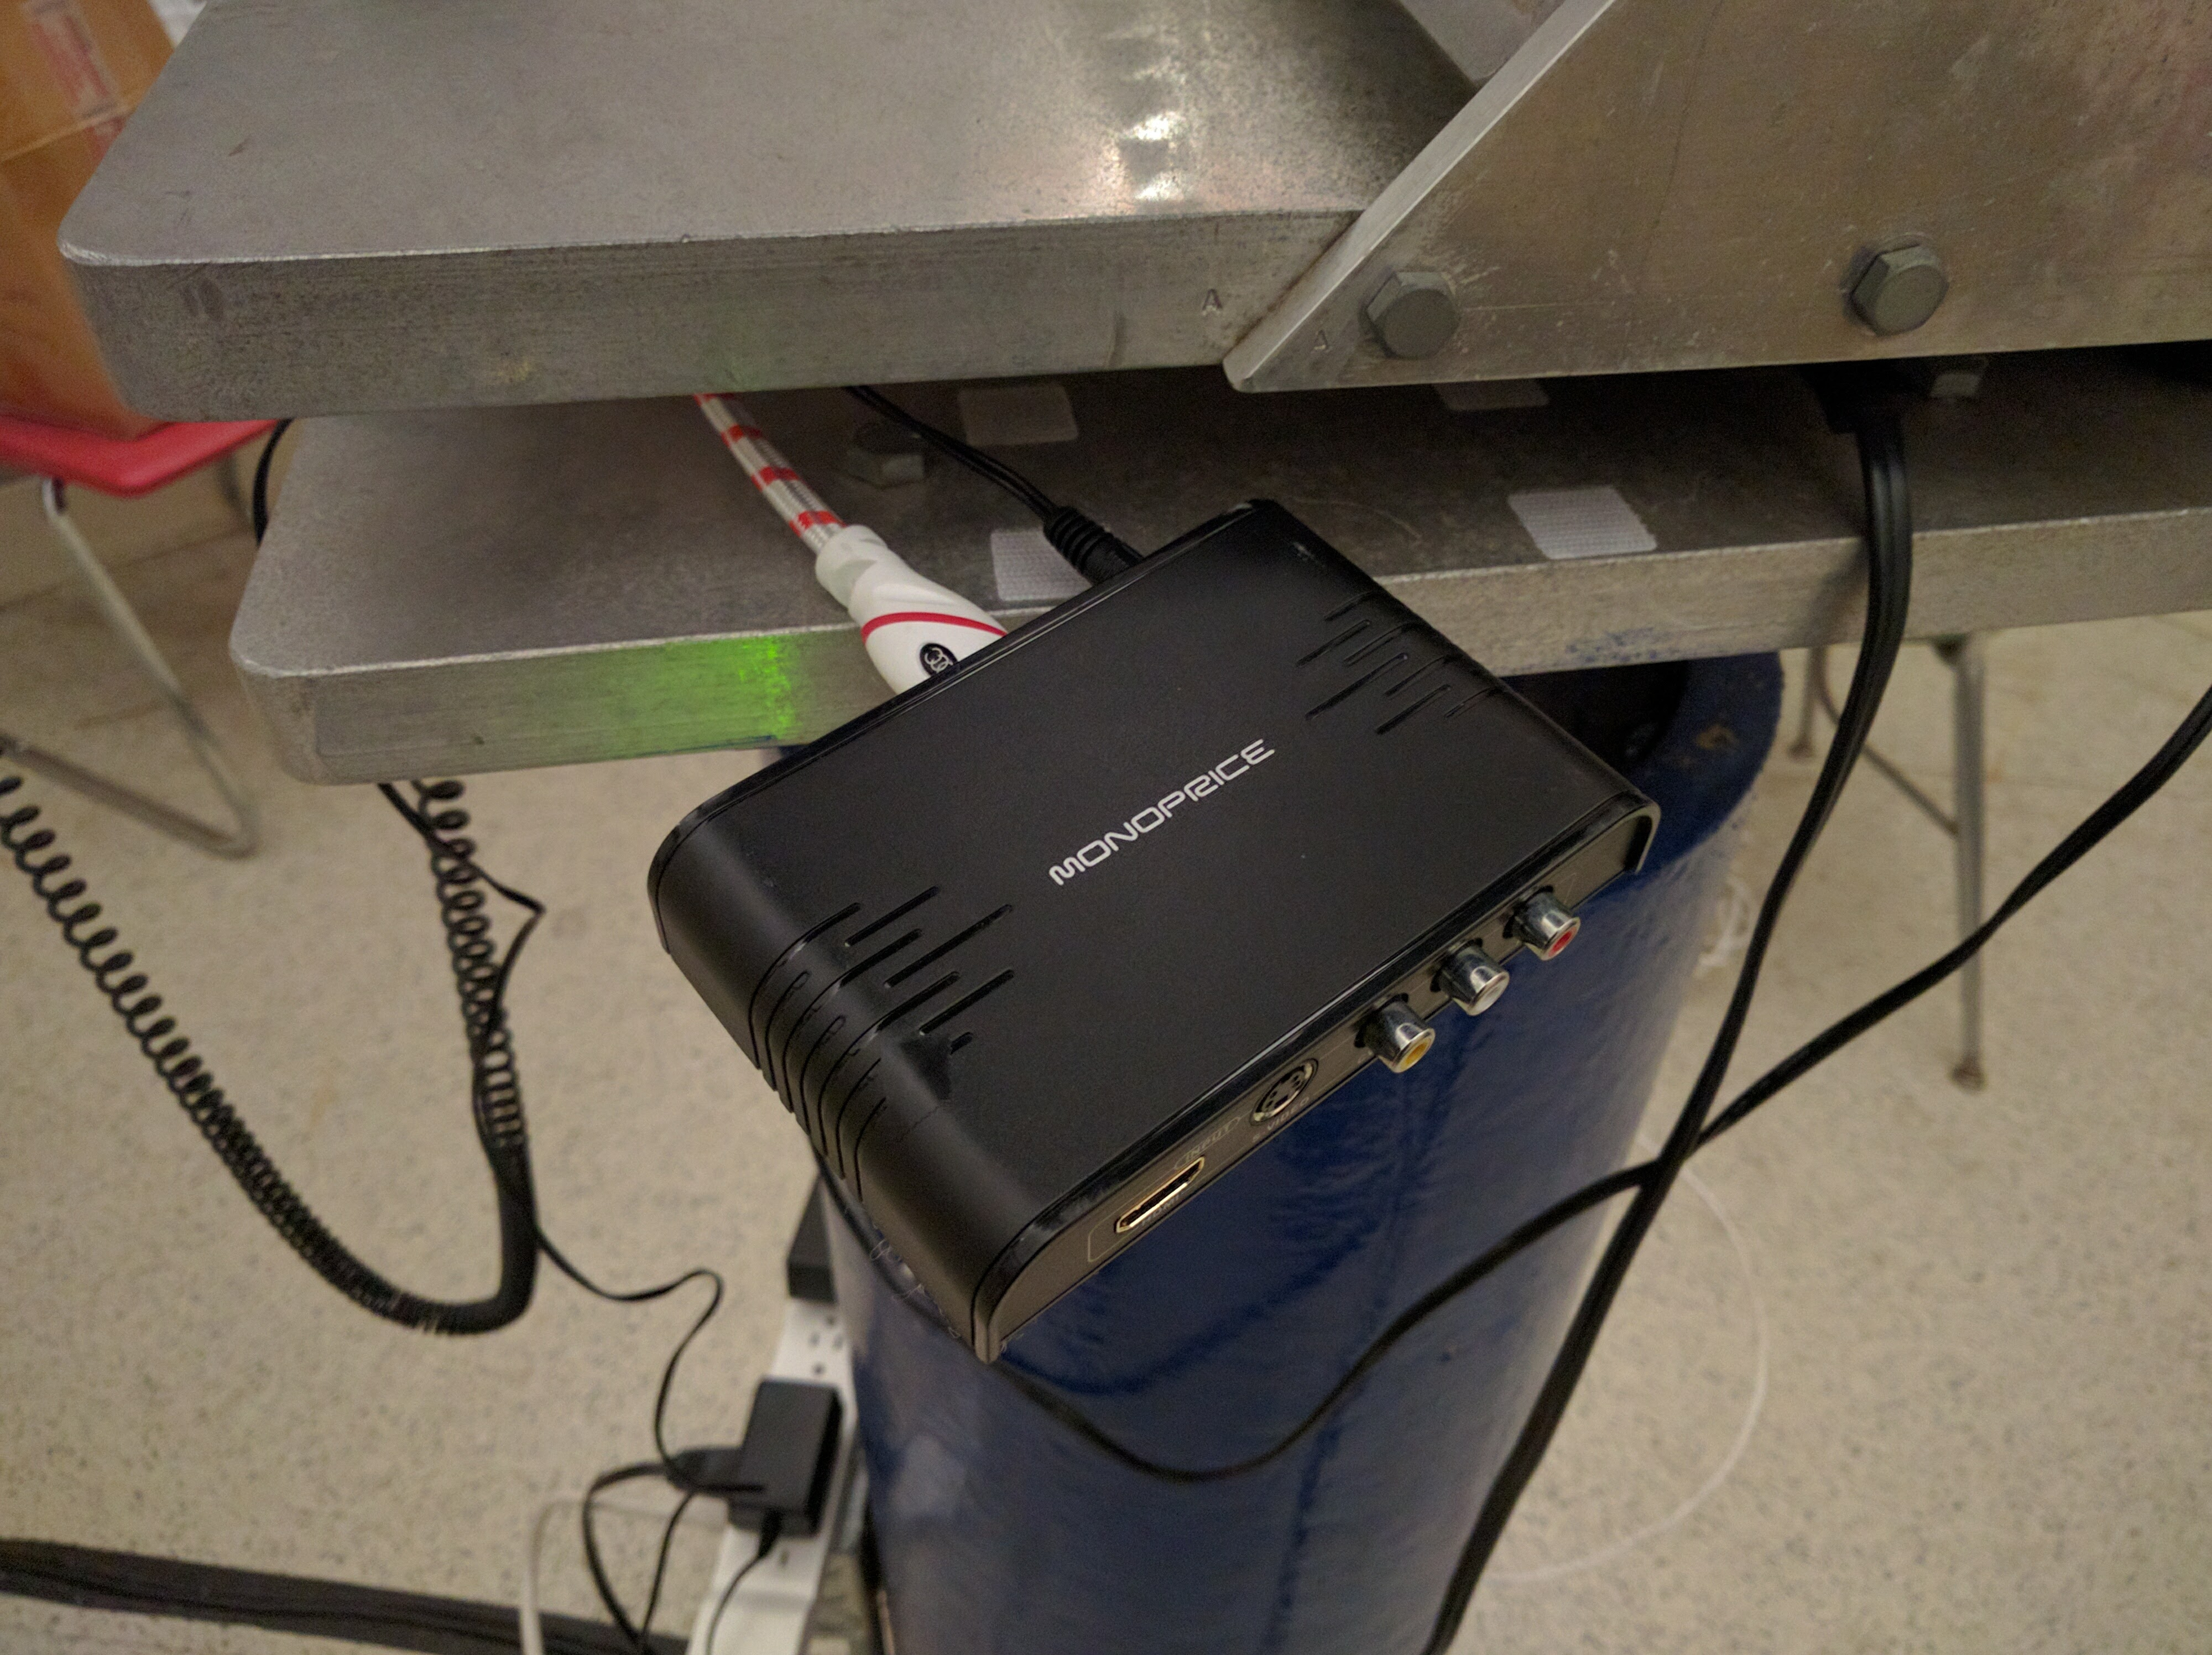
\includegraphics[width=.5\textwidth]{./images/MallinCam/astrofest_setup/converter_box.jpg}}

\end{longtable}
\begin{longtable}{c}    
    \multicolumn{1}{m{\textwidth}}{\step It is time to mount the MallinCam to the telescope. The MallinCam should not be exposed to ambient light. Shut the dome lights off and cover the telescope. One person should mount the MallinCam while another uncoils the cables to prevent them from catching.} \\[2em]
\end{longtable}
\begin{longtable}[t]{cc}
	
	\multicolumn{1}{m{.5\textwidth}}{\step Loosen the screws around the eyepiece and remove it. Remove the cap from focal reducer and insert it into the star diagonal and tighten the thumb screws. The MallinCam should sit flush against the diagonal. It may need to be wiggled a bit in order to push it all the way in. You may turn the red dome lights on to complete the setup but DO NOT remove the telescope cover.} 
    & 
    \raisebox{-.5\totalheight}{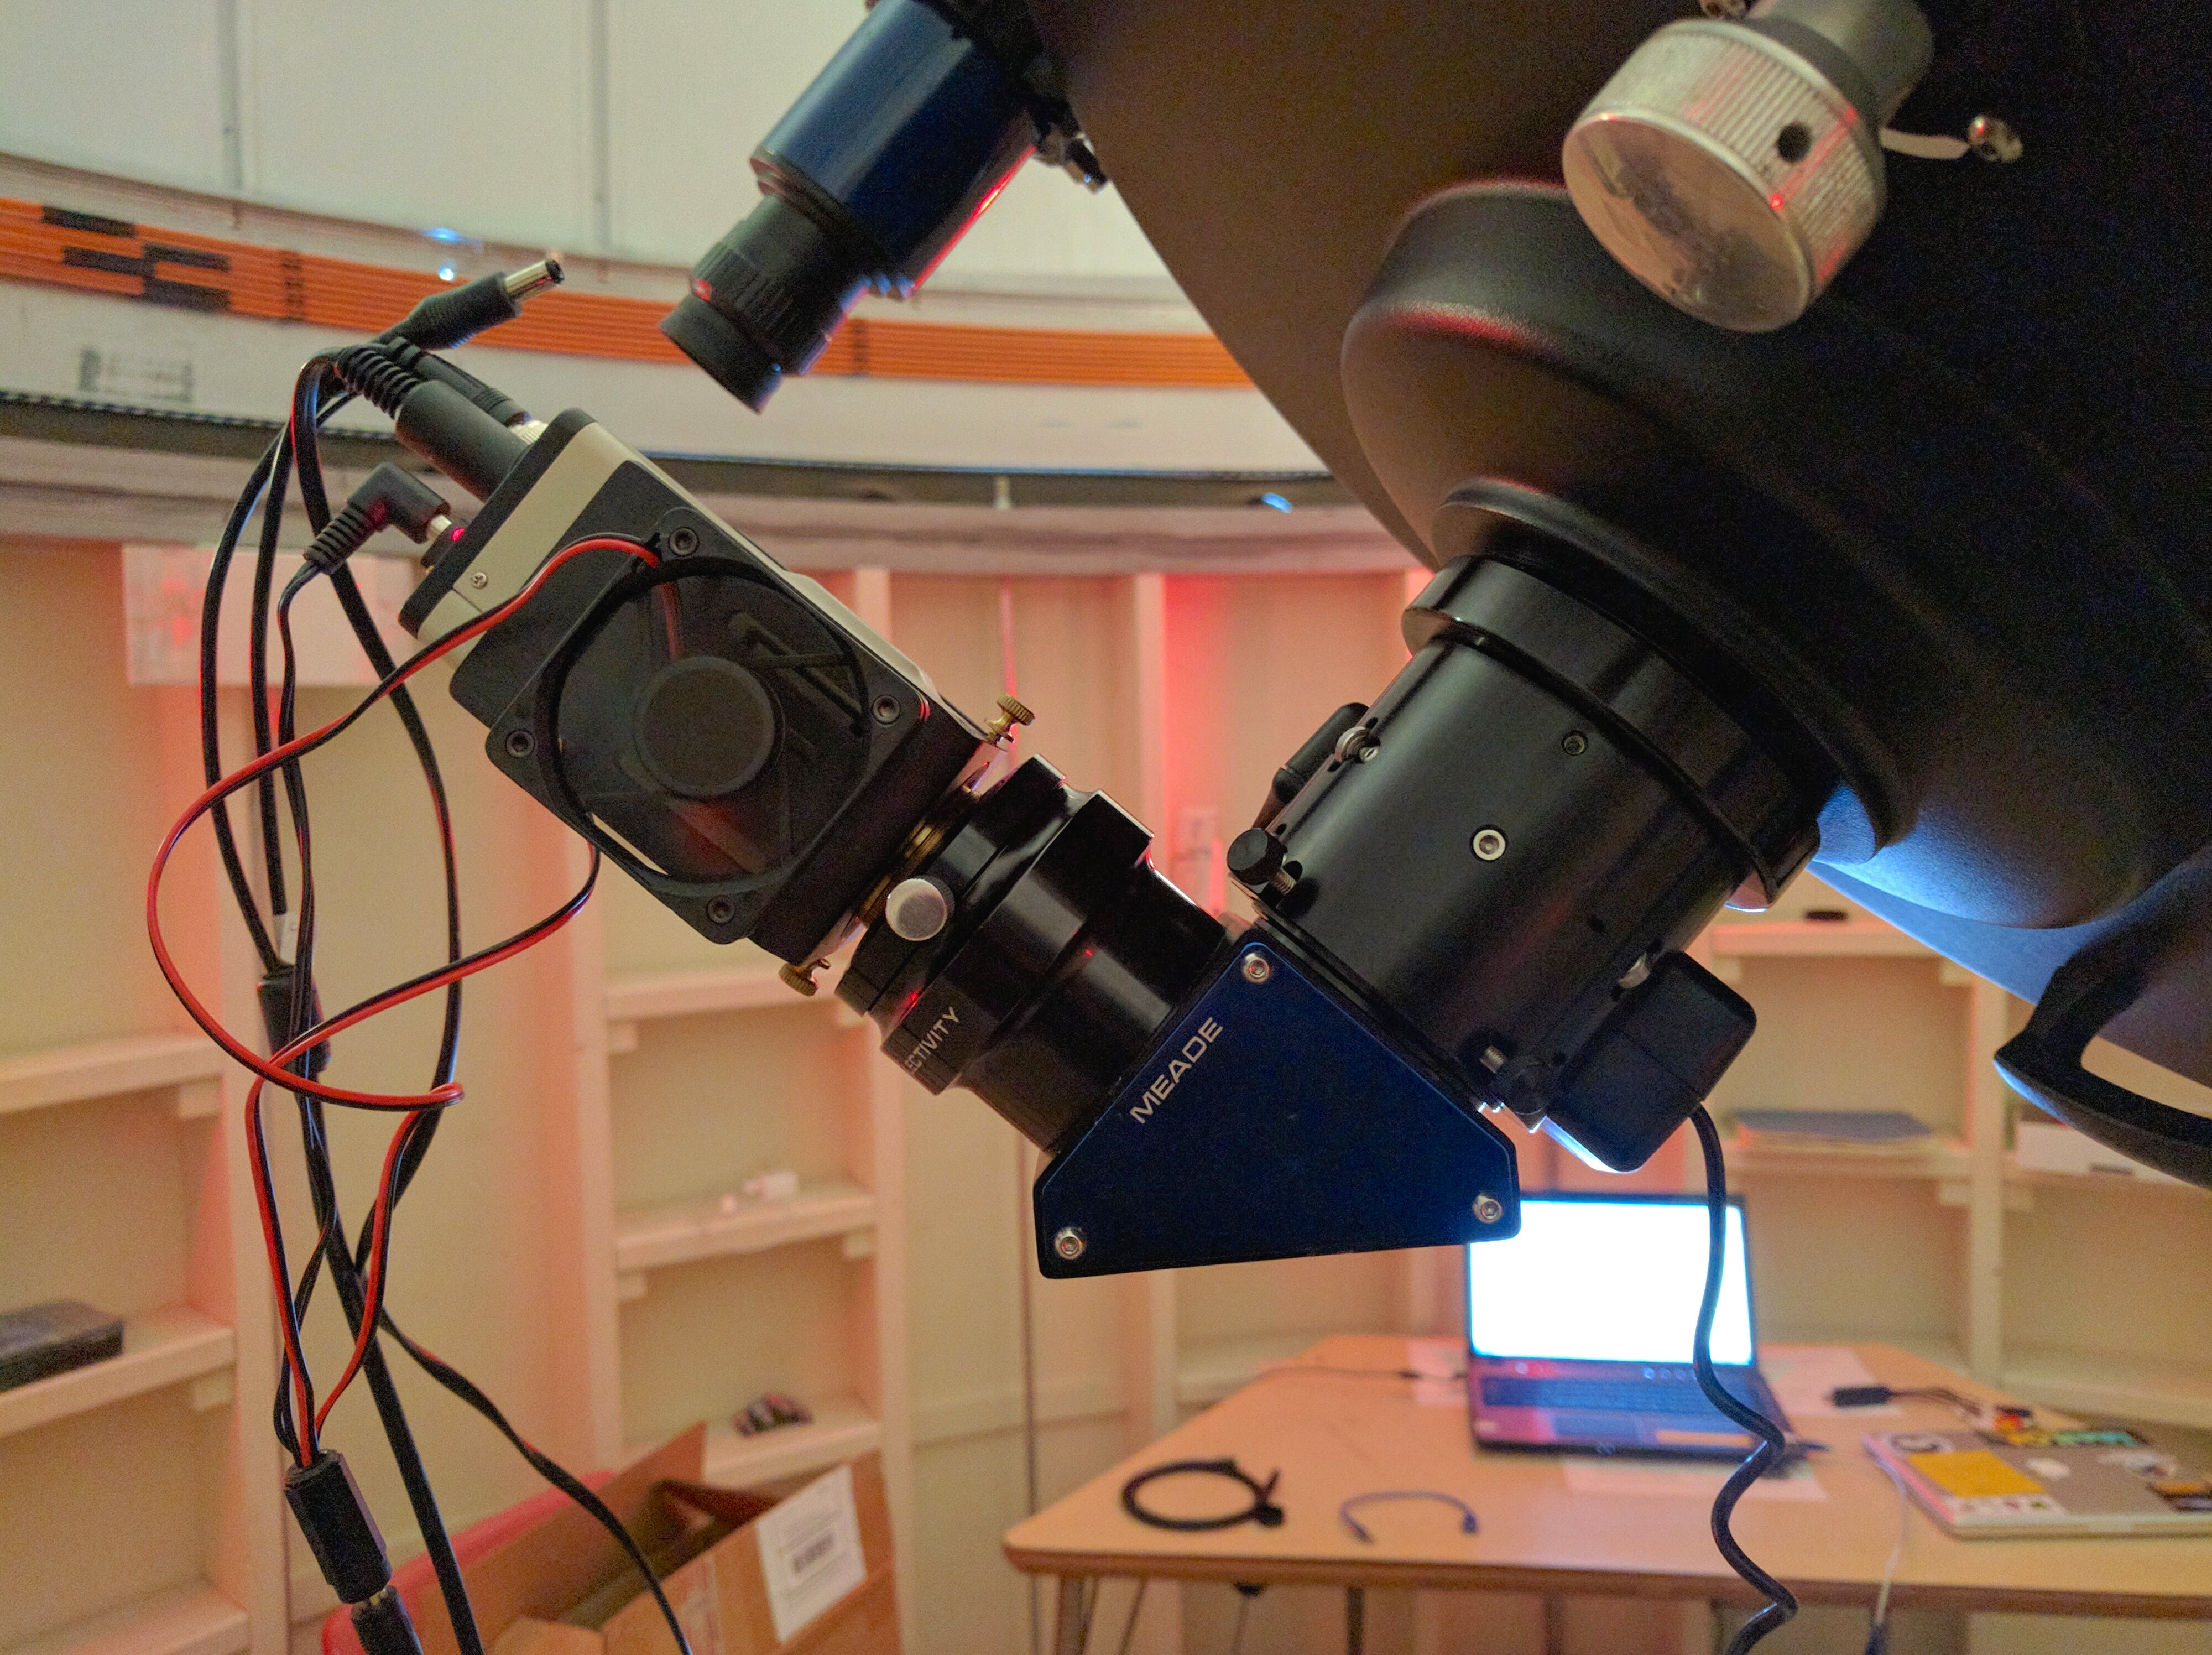
\includegraphics[width=.5\textwidth]{./images/MallinCam/astrofest_setup/mount_camera.jpg}}\\[8em]
	
	\multicolumn{1}{m{.5\textwidth}}{\step Collect the tangled mess of cables at your feet and tie them together with bread ties. Keep them between the chair legs to prevent tripping.
	\vspace{4em} 
    \par \step Plug one end of the S-Video cable into the S-VHS input on the MallinCam and the other end into the S-video input on the converter box.} 
    & 
    \raisebox{-.5\totalheight}{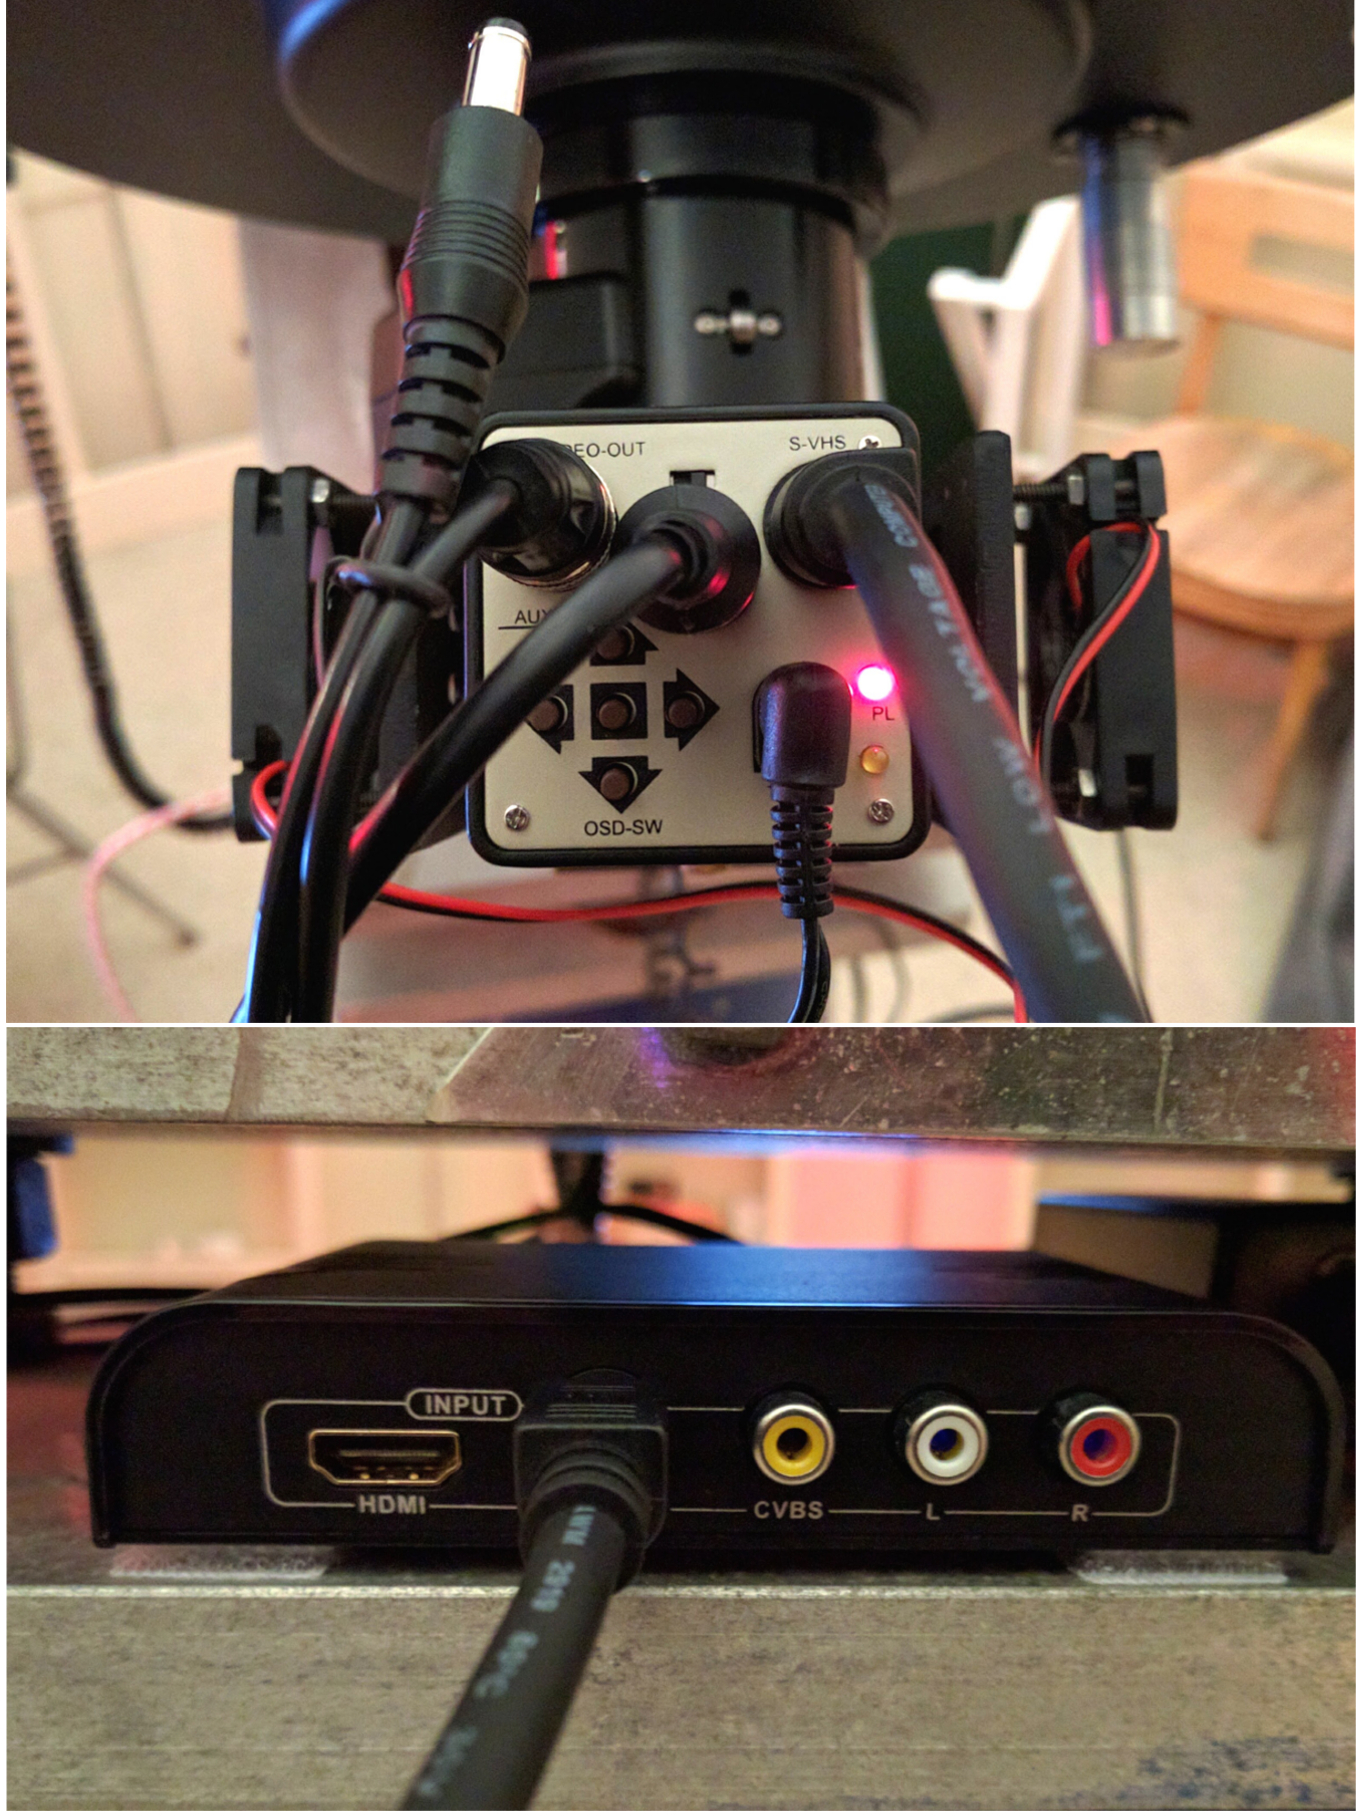
\includegraphics[width=.5\textwidth]{./images/MallinCam/astrofest_setup/svideo12.jpg}}\\
    
    \multicolumn{1}{m{.5\textwidth}}{\step Plug in monitor power. Plug the other end of the HDMI cable into the HDMI Input 1 on the monitor. Turn on the monitor and navigate to Input 1. If "No Signal" message appears on monitor, press the Switch button on the back of the HDMI converter box until a signal appears on the monitor.} 
    & 
    \raisebox{-.5\totalheight}{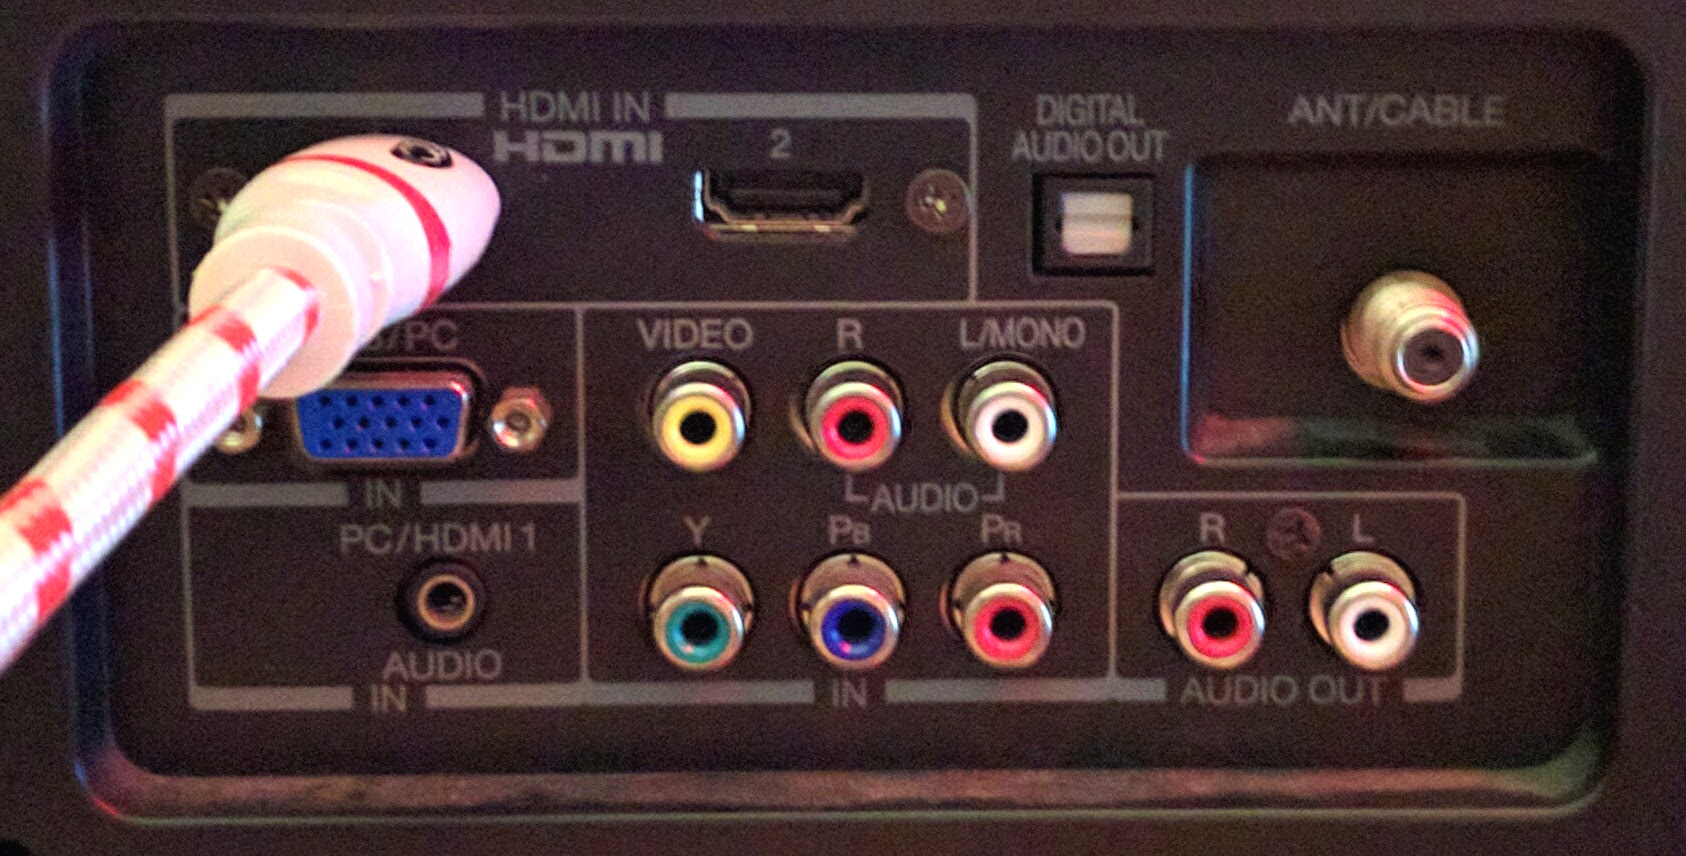
\includegraphics[width=.5\textwidth]{./images/MallinCam/astrofest_setup/HDMI_monitor.jpg}}\\[4em]
	
\end{longtable}
\begin{longtable}{c}    
    \multicolumn{1}{m{\textwidth}}{\step The converter box has two HDMI output options: 720p @ 60Hz and 1080p @ 50Hz, which can be toggled via the 720/1080p button on the back of the converter box. The 720p @ 60Hz option is only recommended for viewing very fast transient events (eg. occultation, satellite transit.)} \\[2em]
    
    \multicolumn{1}{m{\textwidth}}{\step Test the S-Video-to-HDMI connection by turning on color bars in Miloslick.} \\
    
    \multicolumn{1}{m{\textwidth}}{\step Remove the cover from the front of the telescope. By default, the MallinCam is in video mode (1/60s - 1/12000s exposure time). In the CAMERA SETTINGS pane, change the exposure mode to SenseUp mode (33.3ms - 2.13s).} \\
   
    \multicolumn{1}{m{\textwidth}}{\step Slowly increase the exposure time until the outline of the out of focus "donut" becomes visible.}\\
    
    \multicolumn{1}{m{\textwidth}}{\step To bring the star into focus from the 40mm eyepiece to the MallinCam, turn the coarse manual focus knob on the telescope $\sim$3 3/4 turns, counterclockwise. Simultaneously, decrease the exposure time in Miloslick so as not to overexpose the CCD. Fine focus adjustments can be made using the microfocuser on the Autostar II hand controller.}\\
    
   \multicolumn{1}{m{\textwidth}}{\step The MallinCam should now be in focus. From here, slew to your target object and adjust camera settings and exposure time as necessary to observe the target. Video Mode allows the MallinCam to image daytime objects such as the Sun, as well as bright nighttime objects such as the Moon and some planets. SenseUp Mode is used for imaging fainter planets, along with bright stars. Hyper Mode is used for imaging very faint deep sky objects. Several setting profiles have been saved for notable targets that can be used as a template. They can be accessed in Miloslick by clicking File $>$ Open Settings $>$ Select an .mc file $>$ Open. Suggested target-specific settings can be found in Appendices J and K of the Mallincam User's Manual \cite{mallincam}.}
\end{longtable}

\begin{longtable}{c}
	\textbf{Shutdown Procedure:}\\    
	
	    \multicolumn{1}{m{\textwidth}}{\step Park the MallinCam. In Miloslick: Camera $>$ Park MallinCam. Wait three minutes for the camera to warm to ambient temperature before disconnecting power.} \\
	    
	    \multicolumn{1}{m{\textwidth}}{\step Turn off the power strip and unplug the MallinCam power cable. Remove all cables from the back of the MallinCam. Remove the camera from the star diagonal and immediately replace the cover on the focal reducer.} \\
	    
	   \multicolumn{1}{m{\textwidth}}{\step Remove the fan kit from the MallinCam. If you've recently done the dew-prevention procedure, you can store the MallinCam with the focal reducer attached.} \\
	    
    \multicolumn{1}{m{\textwidth}}{\step Cap all cables and return them to their storage containers. Coiling and storing cables properly will extend their life. All MallinCam components and accessories should be stored in the same box. Primary components (MallinCam, focal reducer, fan kit, etc.) should be stored in the blue lunchbox.} \\
    
    \multicolumn{1}{m{\textwidth}}{\step Follow Steps \ref{enum:quickshutdown_start}-\ref{enum:quickshutdown_end} of the Quick Setup Guide (Sec. \ref{ssec:betsy_quick}) to shut down the telescope.} \\
\end{longtable}
\setcounter{rowcount}{0}

\subsection{Streaming with YouTube Live and OBS}
\subsection{Maintenance}
\subsubsection{Dust Removal} \label{sssec:dust}

\begin{figure}[H] 
	\begin{center}
		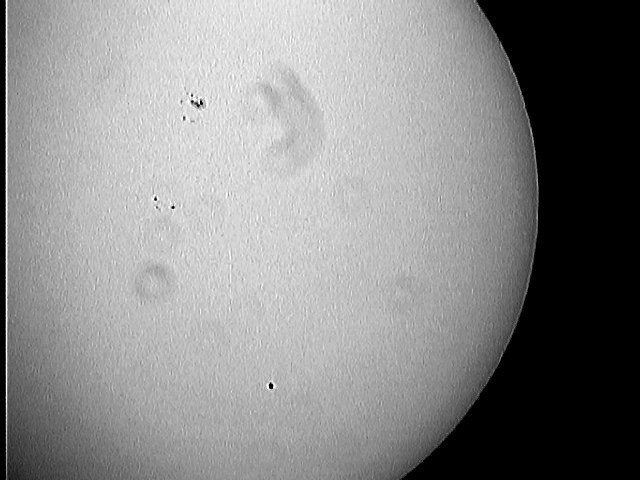
\includegraphics[width=.95\textwidth]{./images/MallinCam/dust/mercury_transit.jpg} 
		\caption{A MallinCam image of the sun taken during a transit of Mercury.
		Out-of-focus dust "donuts" are visible throughout the entire image.}
		\label{sundust}
	\end{center}
\end{figure}

Unlike most CCD cameras, the MallinCam does not output raw pixel counts so artifacts due to the presence of dust on the sensor cannot be removed using standard preprocessing techniques.
Therefore, the only way to deal with the dust is to remove it from the front of the sensor.
The procedure described below can be applied to any eyepiece or objective.
A good rule of thumb for cleaning telescope optics is to do so \textit{only when absolutely necessary}.
Too-frequent cleaning can strip the coating on the lenses and dust accumulation can be prevented by keeping the optics covered when not in use.
Most of the materials required for this procedure can be found in the front pocket of the blue lunchbox where the camera is stored.
You will need:

\begin{longtable}[t]{cc}
	\multicolumn{1}{m{.4\textwidth}}{
		\begin{enumerate}[label=\protect\circled{\arabic*}]
	\item Rubber bulb blower
	\item Magnifying glass
	\item 91\% or 99\% isopropyl alcohol (anything lower than 91\% will leave streaks)
	\item Microfiber cloth
	\item Small cotton swab
	\end{enumerate}}

	&		
			
	\raisebox{-.5\totalheight}{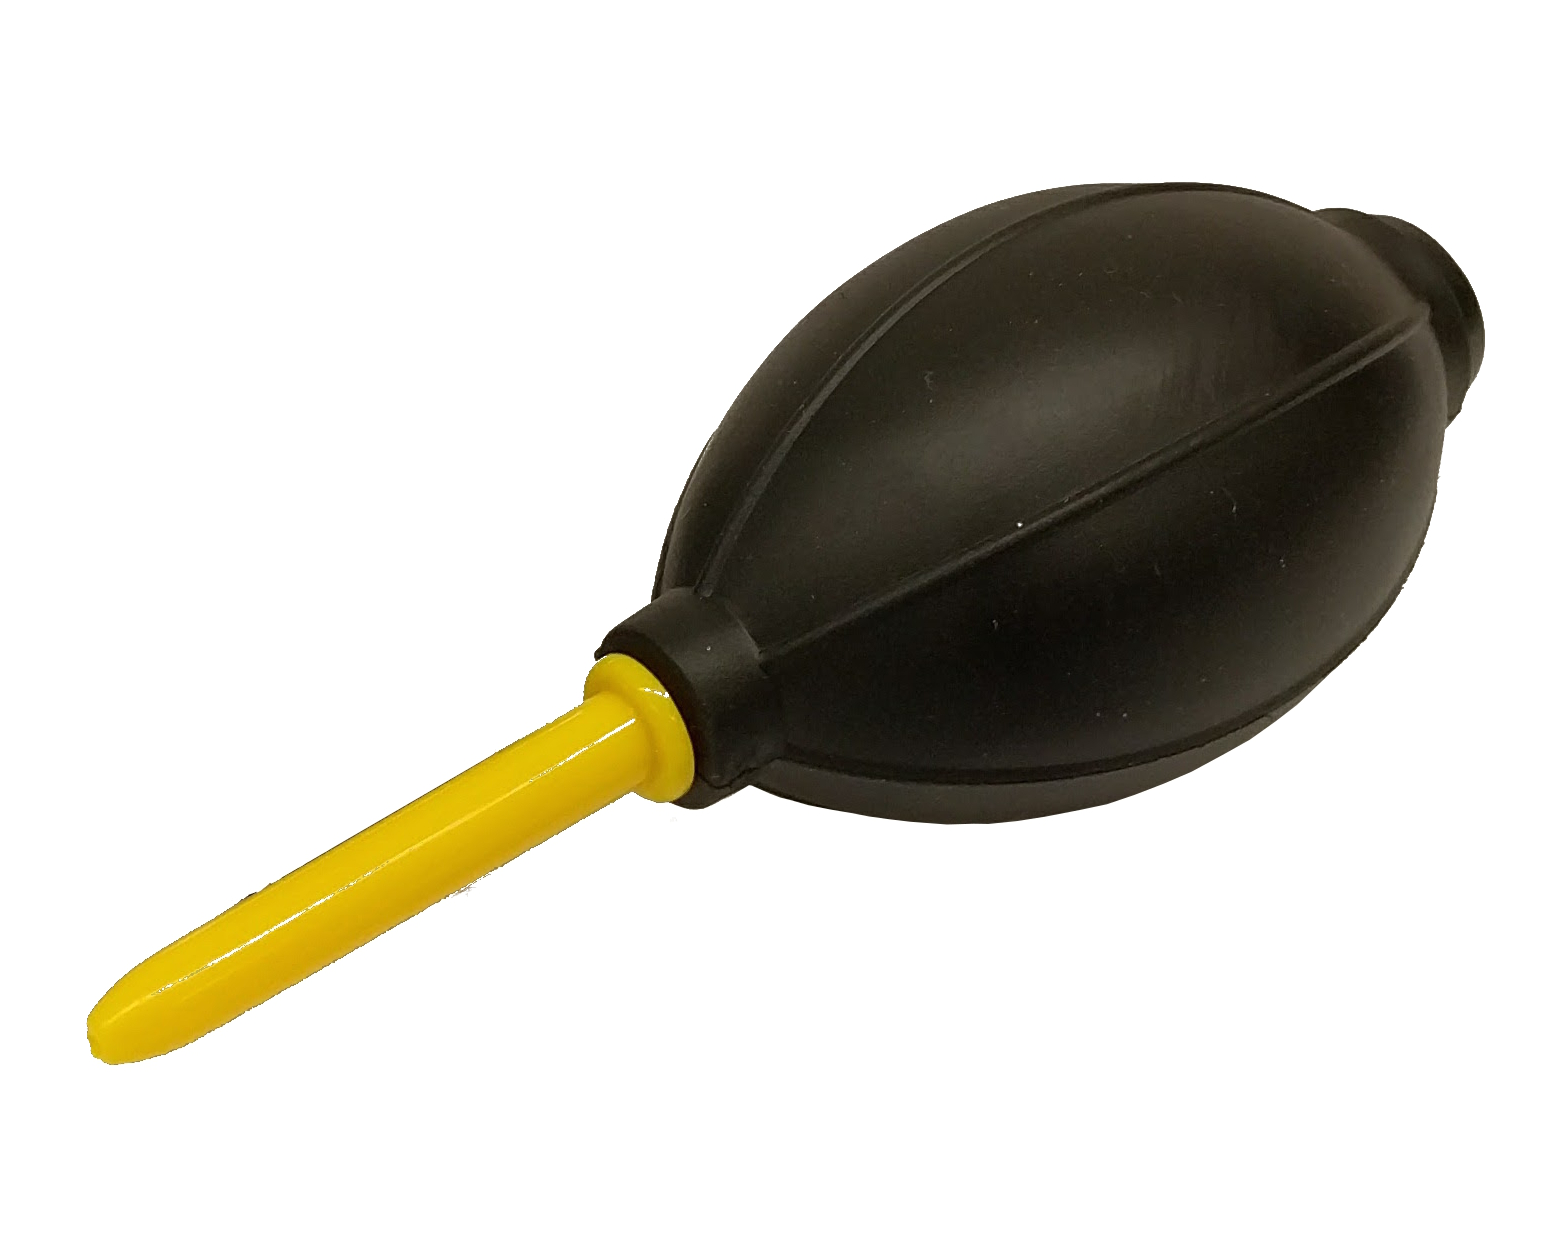
\includegraphics[width=.4\textwidth]{./images/dust/blower.jpg}}
\end{longtable}

The following procedure requires extreme care, a delicate touch, and a bit of guts:
\begin{enumerate}
	\item First try to blow the dust off with the rubber bulb blower
	\footnote[*]{\textbf{Never blow breath directly or use compressed air on telescope optics.}}
	\item If that doesn't work, wrap the microfiber cloth around the end of the cotton swab and dampen (don't soak) the cloth with alcohol.
		Try not to touch the cloth too much with your fingers.
	\label{enum:duststart}
	\item Very gently drag the tip of the cloth across the sensor in one direction.
	Apply almost no pressure at all, making several gentle passes in the same direction to clean the rest of the sensor.
	Avoid touching the pins around the edge of the sensor.
	\label{enum:dustend}
	\item After the sensor dries, inspect it with a magnifying glass under light at an angle.
	If it's still dusty, repeat steps \ref{enum:duststart} and \ref{enum:dustend} once.
\end{enumerate}


\subsubsection{Dew and Frost Prevention} \label{sssec:dew}

\begin{figure}[H]
	\begin{tikzpicture}
    
    \begin{scope}[xshift=-1mm, yshift=0cm]
    \node {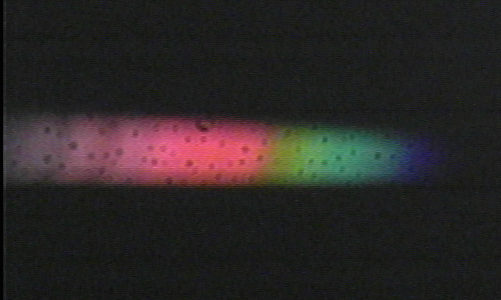
\includegraphics[width=.59\textwidth]{./images/mallincam/dew/dew_spectrum.png}};
    \end{scope}    
    
    \begin{scope}[xshift=.5\textwidth, yshift=0]
    \node {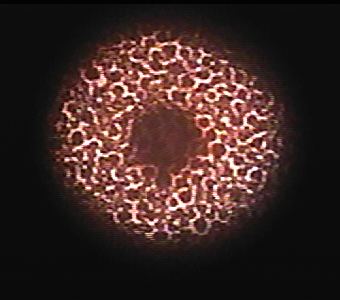
\includegraphics[width=.4\textwidth]{./images/mallincam/dew/frost.png}};
    \end{scope}
    
	\end{tikzpicture}
	\caption{In the image of a stellar spectrum on the left, dark spots can be seen as condensation forms on the sensor.
				In the image of an out-of-focus star on the right, the condensation has turned to frost resulting in a 
				marbling pattern.}
\end{figure}


The MallinCam is equipped with a very efficient Peltier cooling system capable of cooling the CCD to 27$\deg$ F below ambient.
When moisture in the air is exposed to the chip at higher cooling levels, it will condense on the sensor.
At the highest cooling levels, the dew will freeze on the sensor.
Repeated frost buildup has the potential to damage the CCD.
The only way to prevent moisture from condensing on the sensor is to seal dry air inside the chamber around the CCD.
The following procedure is adapted from Woody Schlom's dew prevention guide.
We use the MFR-5 focal reducer to seal the chamber but, if no focal reduction is desired, another optically flat element can be used.
Any of the MFR-5 configurations from Appendix \ref{sssec:focal_reduction} may be used, as long as there is at least one piece of glass
isolating the CCD from the outside air.
The procedure can be extended to dehumidify other instruments.
You will need:

\begin{longtable}[t]{cc}
	\multicolumn{1}{m{.5\textwidth}}{
		\begin{flushleft}
			\begin{enumerate}[label=\protect\circled{\arabic*}]\small
				\item Silica gel canister
				\item Gallon-sized Ziploc bag
				\item MallinCam XII
				\item MFR-5 Focal Reducer
				\item Oven
			\end{enumerate}
		\end{flushleft}}
	&		
	\raisebox{-.5\totalheight}{
\includegraphics[width=.25\textwidth]{./images/MallinCam/dew/silica_gel_can.jpg}}
\end{longtable}   

\setcounter{rowcount}{0}
\begin{longtable}[t]{ccc}
	\multicolumn{1}{m{.425\textwidth}}{\step If the silica gel is saturated with moisture, the pellets will be pink.
										Remove the cartridge from the canister and place it in the oven at 350$\deg$ F
										until the pellets turn blue. The gel is now desaturated and capable of absorbing moisture.} 
    & 
    \raisebox{-.5\totalheight}{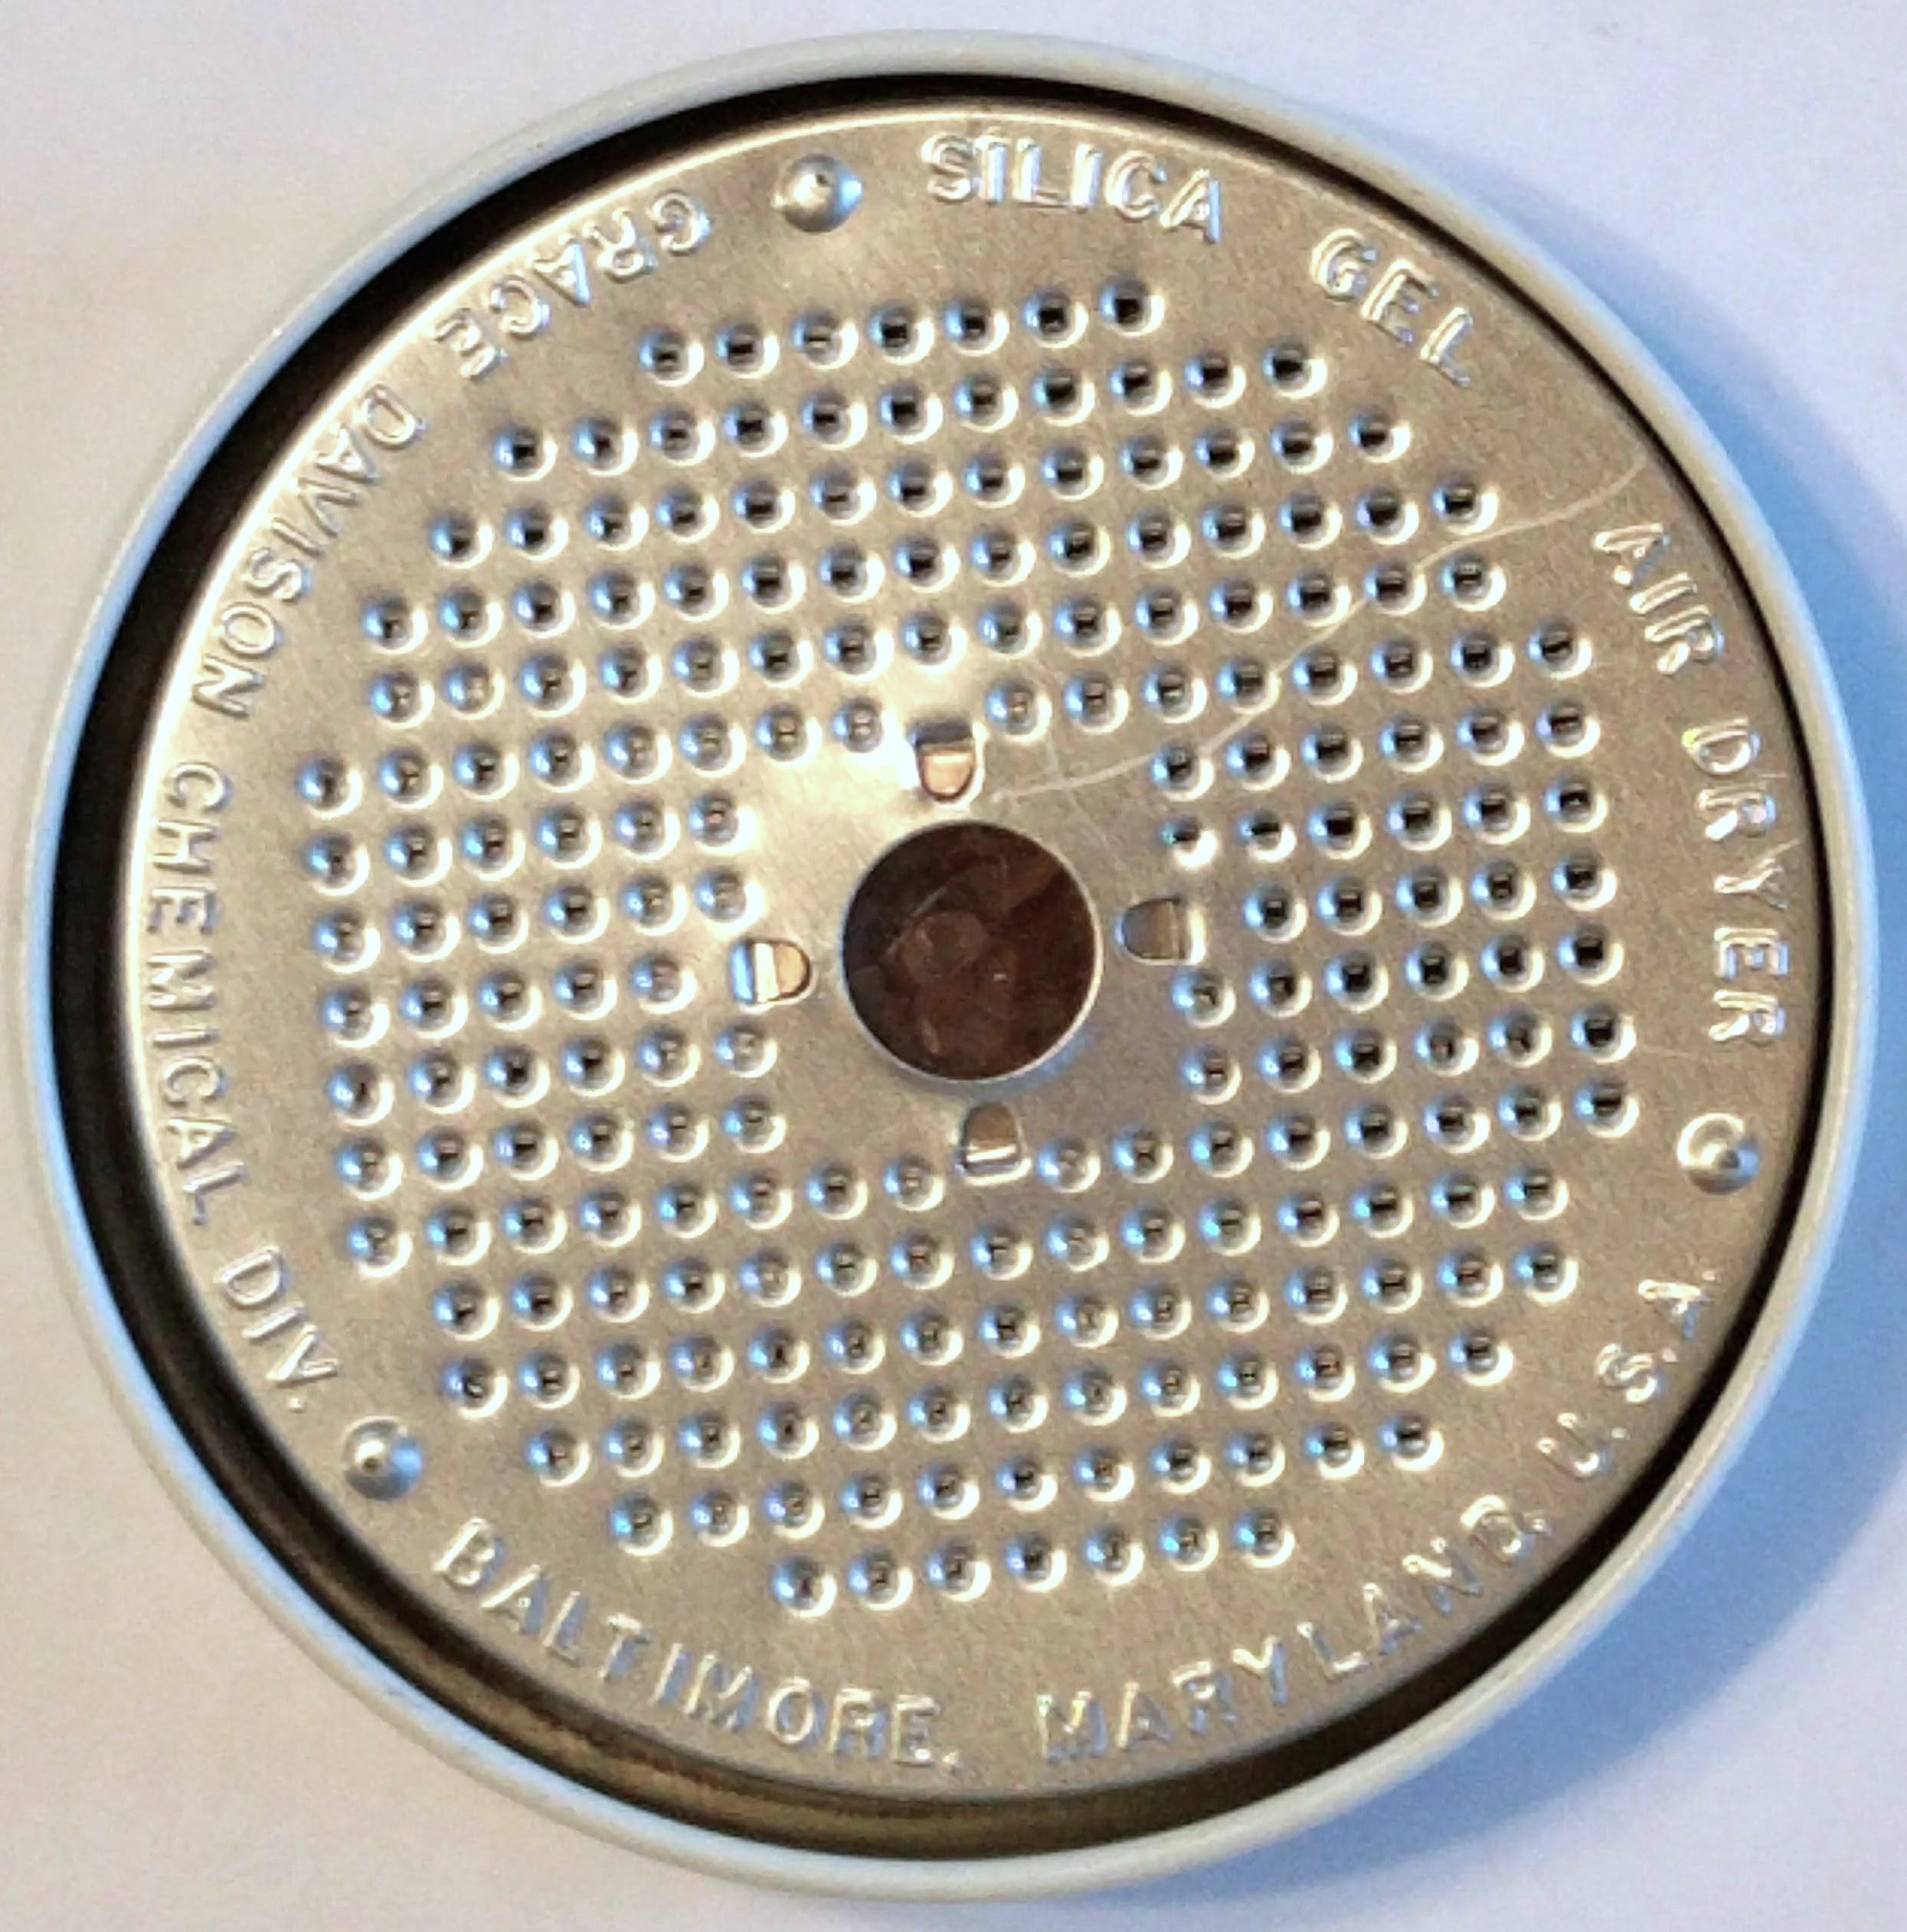
\includegraphics[width=.25\textwidth]{./images/mallincam/dew/silica_sat.jpg}}
	& 
    \raisebox{-.5\totalheight}{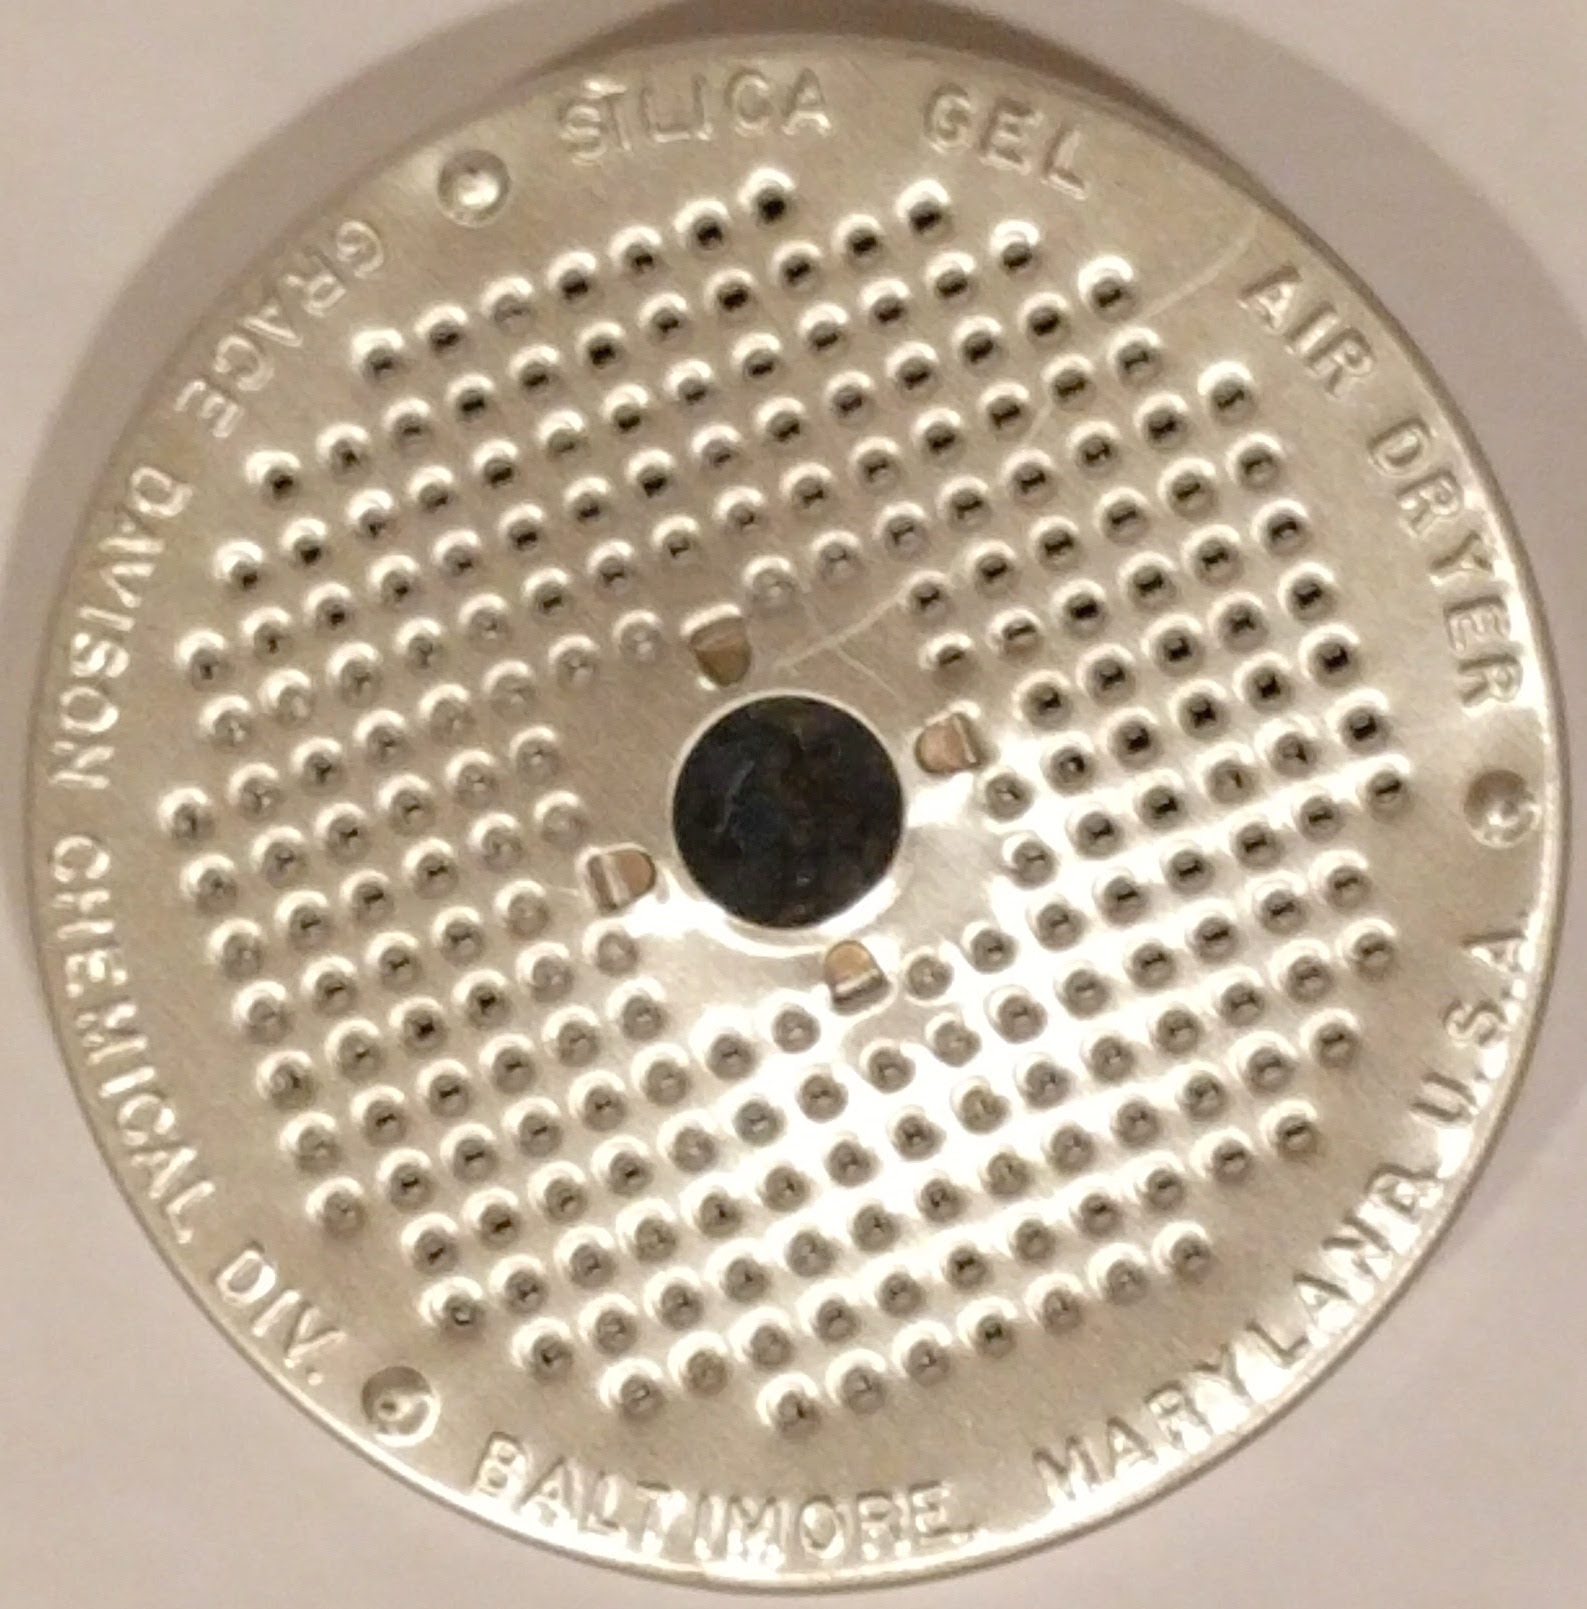
\includegraphics[width=.25\textwidth]{./images/mallincam/dew/silica_desat.jpg}}
\end{longtable}
\begin{longtable}[t]{cc}
	\multicolumn{1}{m{.5\textwidth}}{\step Allow the silica gel cartridge to cool and place it inside the plastic bag along with the 
											MallinCam and focal reducer. Keep the focal reducer capped.
											Seal the bag tightly, ensuring that it is not completely inflated
											or you won't be able to screw the focal reducer in.
											Place the bag in a dark location for at least 12 hours.} 
    & 
    \raisebox{-.5\totalheight}{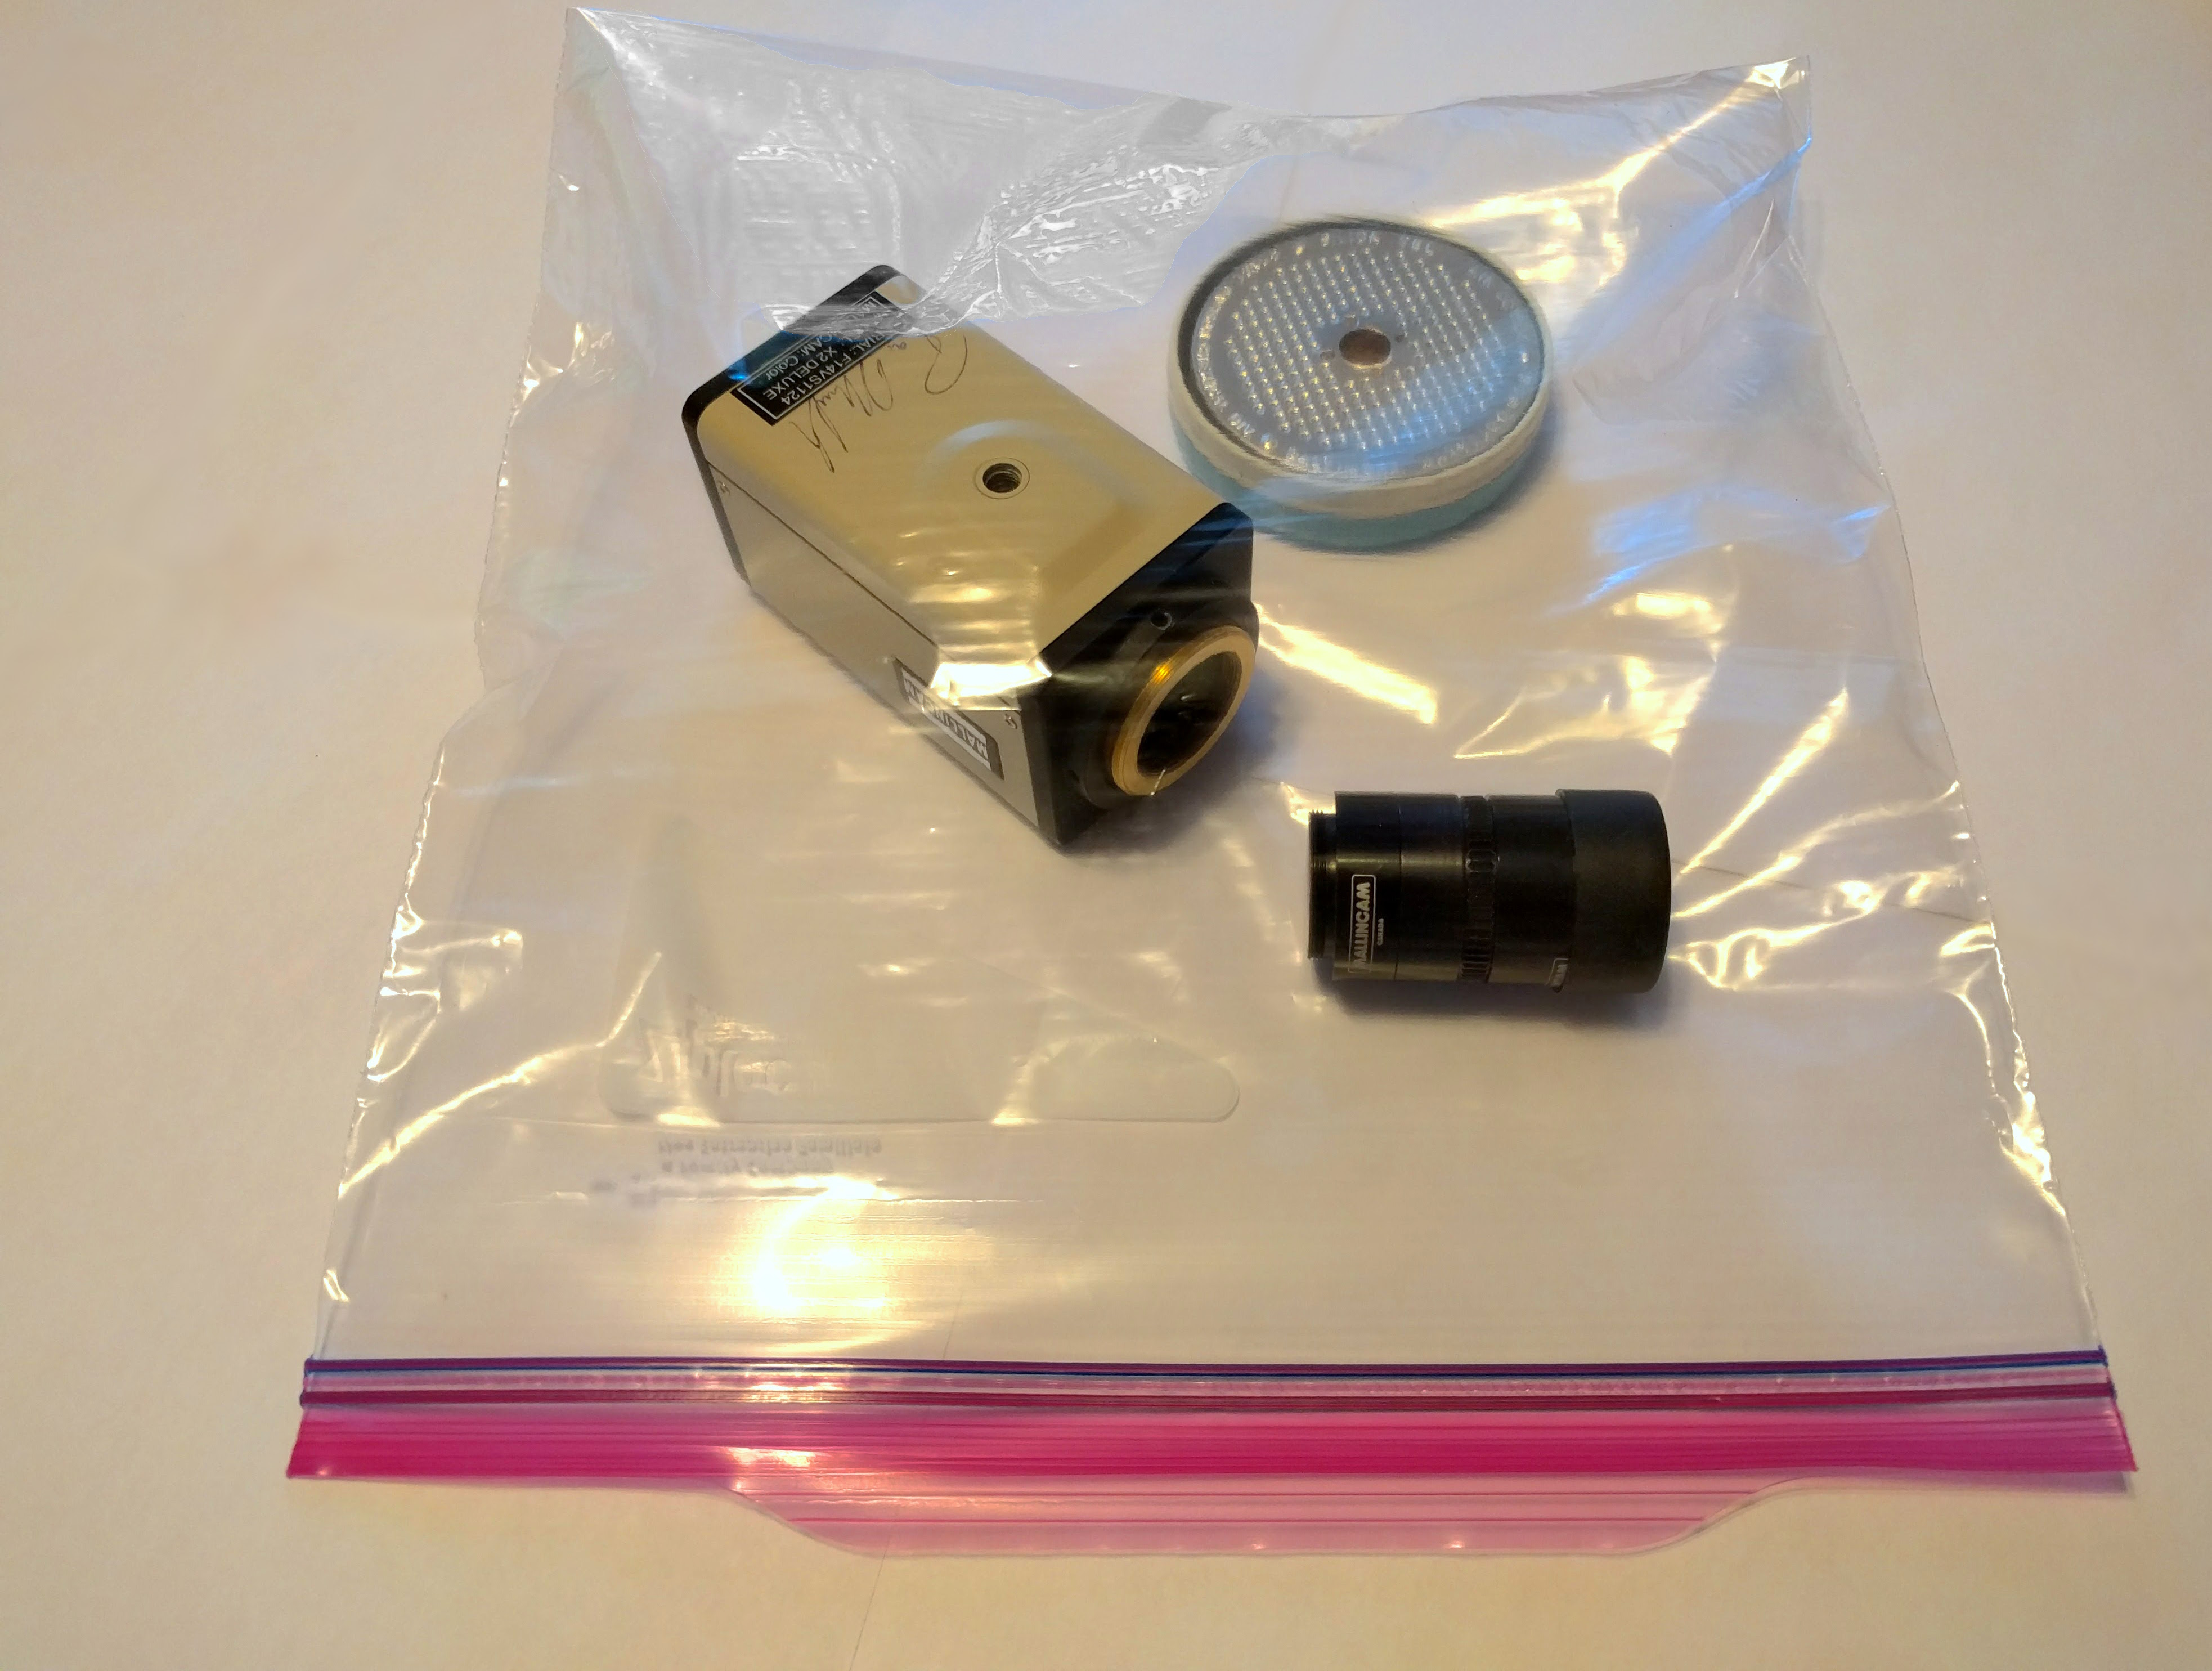
\includegraphics[width=.45\textwidth]{./images/mallincam/dew/unscrewed_in_bag.jpg}}\\[2em]
    \multicolumn{1}{m{.5\textwidth}}{\step \textbf{Without opening the bag}, firmly screw the focal reducer into the MallinCam window, sealing the dry
    										air around the CCD.} 
    & 
    \raisebox{-.5\totalheight}{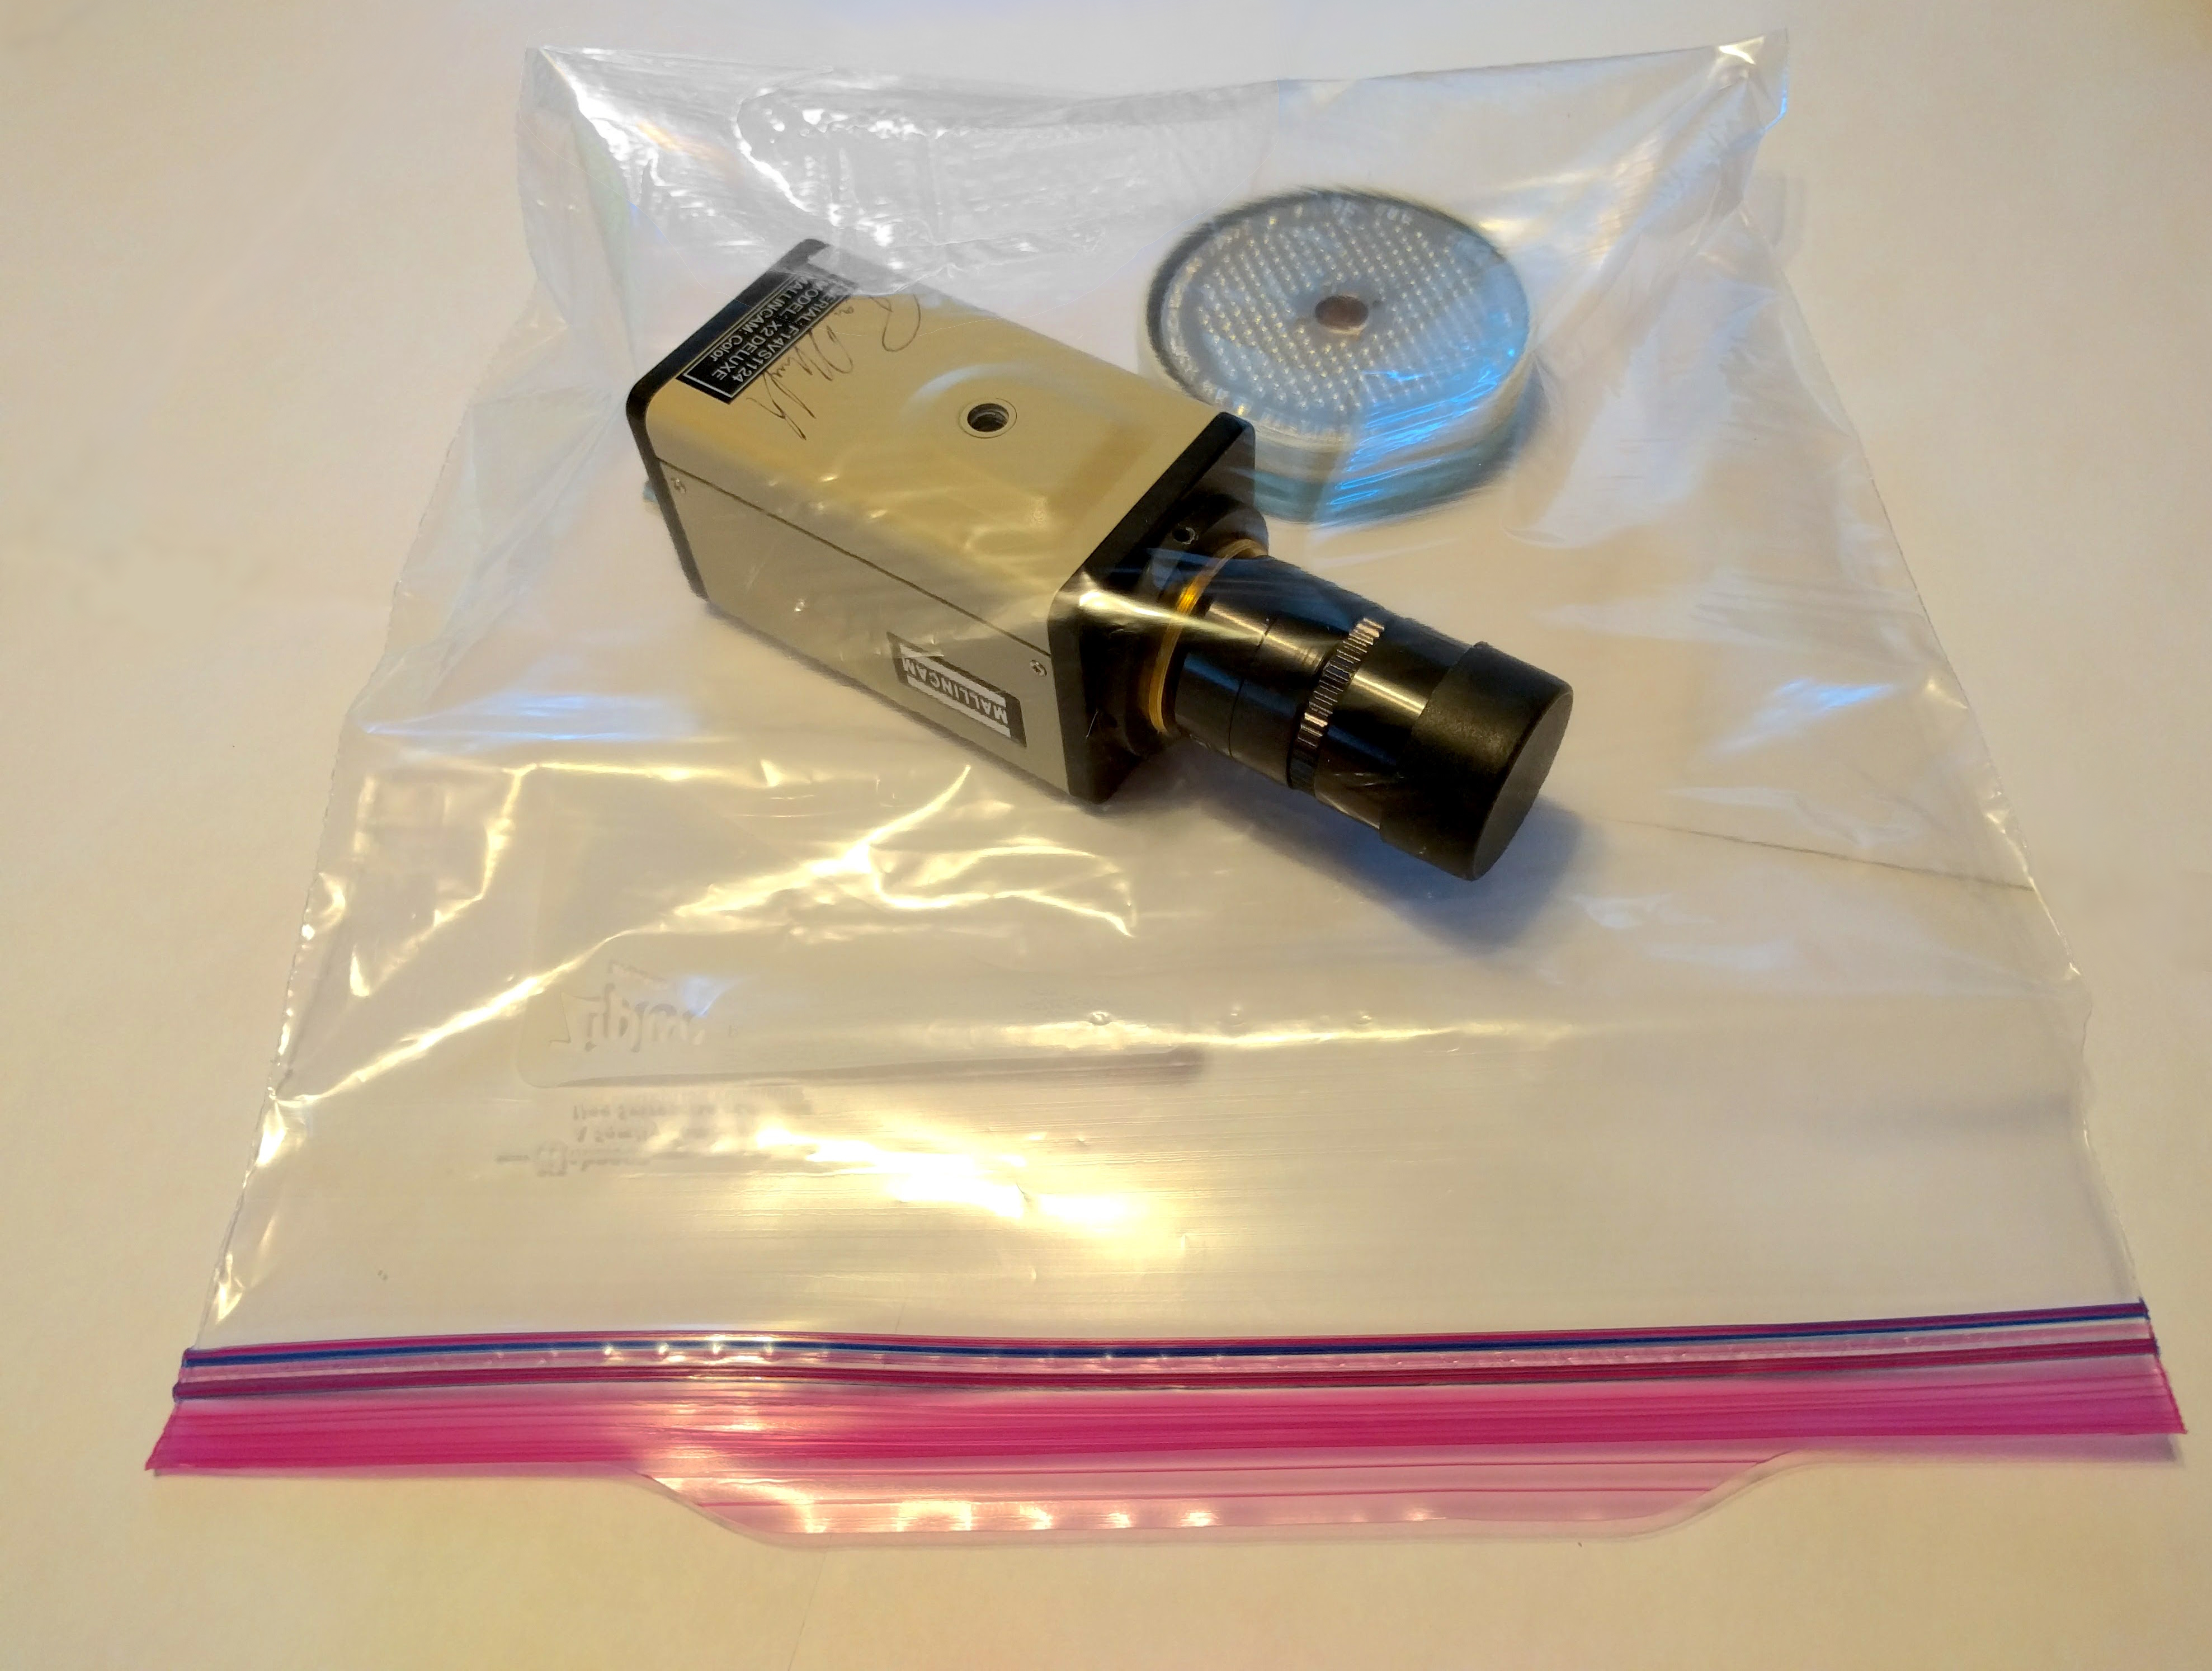
\includegraphics[width=.45\textwidth]{./images/mallincam/dew/screwed_in_bag.jpg}}\\
    \multicolumn{1}{m{.5\textwidth}}{\step Remove the MallinCam from the bag. The camera can now operated at the highest cooling levels without
    										concern for dew or frost. The seal should hold for several months of regular use. If you remove the 
    										focal reducer however, the process will have to be repeated.} 
    & 
    \raisebox{-.5\totalheight}{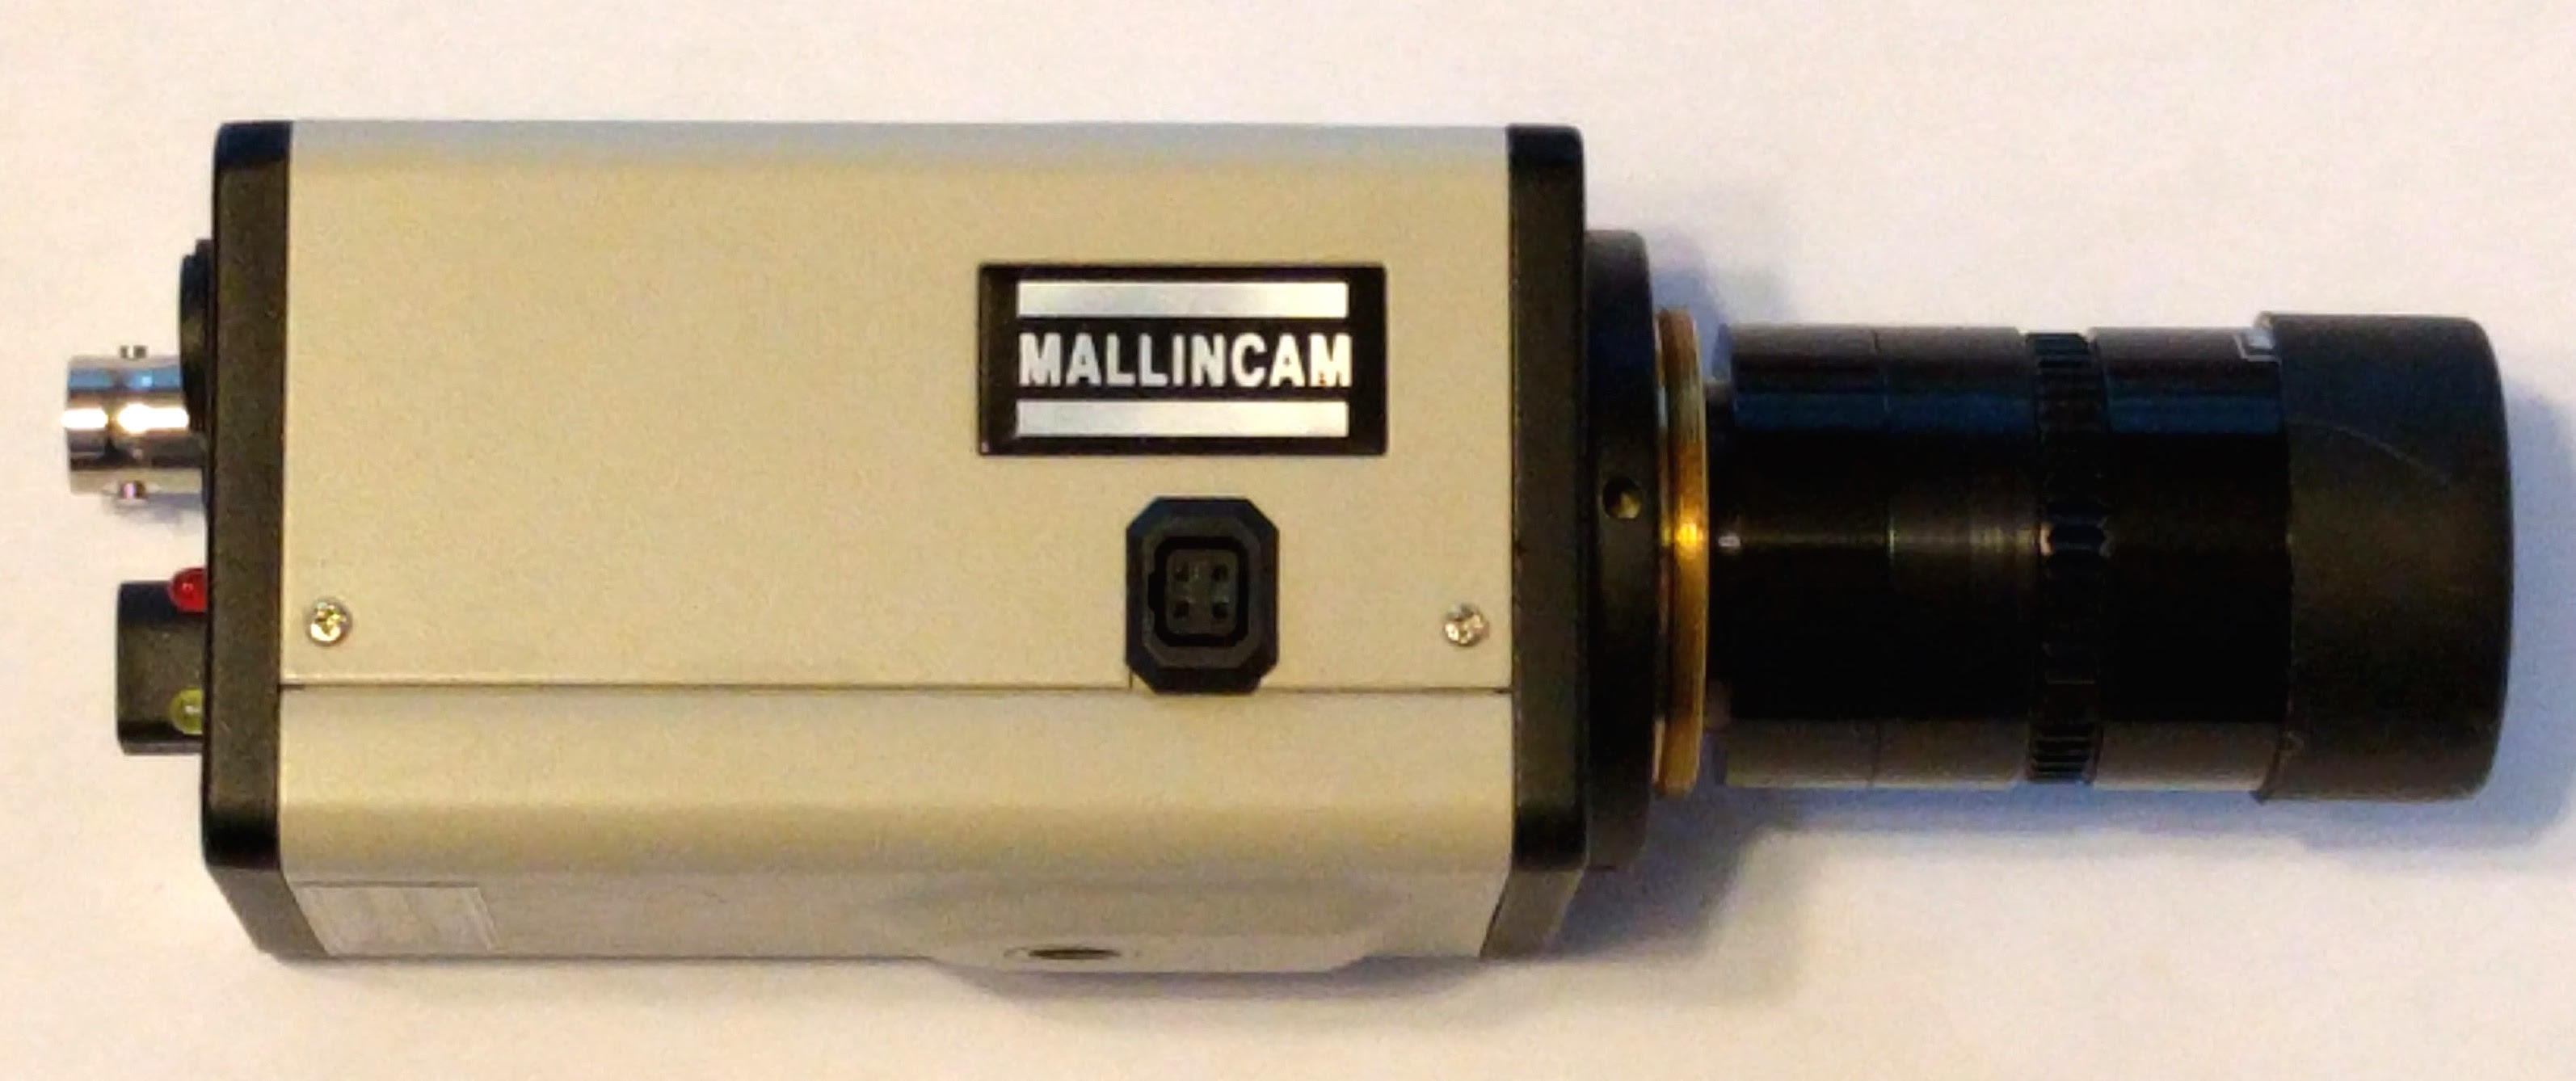
\includegraphics[width=.45\textwidth]{./images/mallincam/dew/mfr5_assembled.jpg}}
\end{longtable}

If operating the camera at low cooling levels in high humidity without sealing the chamber, it helps to set the camera in the telescope before turning the cooling on.
If the telescope is closed-tube, this will provide some seal from the outside air.
Avoid pulling the camera in and out of the telescope unless necessary. 

Despite precautions, if you notice condensation forming, turn MOTION DETECT on by adjusting the following settings using the buttons on the back of the camera:
\begin{enumerate}
	\item[] \quad $>$Press Enter to open menu
	\item[] \quad\quad $>$ Scroll down to MOTION DETECT
	\item[] \quad\quad\quad $>$ Right arrow to toggle MOTION DETECT ON
	\item[] \quad\quad\quad\quad $>$ Press Enter to open MOTION DETECT menu
	\item[] \quad\quad\quad\quad\quad $>$ Set LEVEL to full right and TIMER to 60 seconds
	\item[] \quad\quad\quad\quad\quad\quad $>$ Return
\end{enumerate}
MOTION DETECT is the TEC (Thermal Electric Cooler) for the MallinCam. Setting it to the lowest level provides minimal cooling and allows the sensor to heat up and the condensation to evaporate. This can also be adjusted by the Peltier Cooler setting in Miloslick. Aggressive cooling should only be used when many hot pixels are present in images.


\subsection{MallinCam Troubleshooting}\label{ssec:x2troubleshoot}

\textbf{\flushleft Issues:}
\begin{itemize}
	\item Miloslick: "No MCXtreme X2/PC found on COM6"
	\item Miloslick: "Unknown serial port error"
	\item Miloslick: "No serial ports found"
\end{itemize}
\textbf{Solution:} Go to Windows Control Panel $>$ Devices and Printers. 
If "FT232R USB UART" is listed under "Unspecified", quit Miloslick (leaving camera control plugged in) and restart software.
The order that cables are plugged into the computer matter to the software.
If it's not listed, make sure the MallinCam power is on (red LED indicator).
If it is on, welp, you're on your own buddy.

\textbf{\flushleft Issues:}
\begin{itemize}
	\item Miloslick: "Video Device "USB OEM Device" Not Found"
	\item Miloslick: Blue screen in display window
\end{itemize}
\textbf{Solution:} Go to Windows Control Panel $>$ Devices and Printers.
If "USB OEM" is listed under "Unspecified", quit Miloslick (leaving camera control plugged in) and restart software.
If that doesn't work and you are using Miloslick for the first time on a new computer, the Frame Grabber device drivers will need to be installed via the Frame Grabber installation mini-disk in the front pocket of the blue lunchbox. If the device is still not listed, the frame grabber may be damaged.

\textbf{\flushleft Issue:} MallinCam is frozen or not responding to commands.\\
\textbf{Solution:} First, confirm the camera is in fact frozen by turning on the color bars in Miloslick and via the buttons on the back of the camera by pressing and holding the UP and DOWN buttons simultaneously for two seconds. If the color bars turn on via the camera buttons but not from Miloslick, the camera may no longer be connected to the software; refer to the first issue in this appendix. If the color bars do not turn on at all, turn off the MallinCam for 30 seconds, then power up as usual. If the issue is still not resolved, the MallinCam must be reset to its factory default settings by the following procedure:
\begin{enumerate}
	\item Press the CENTER button on the camera for two seconds until the menu appears
	\item Press the UP button once to send the cursor to the last line $<$SAVE$>$
	\item Press the RIGHT button once to change $<$SAVE$>$ to $<$PRESET$>$
	\item Press the CENTER button to select $<$PRESET$>$ and return the camera to its factory settings
\end{enumerate}




\section{Rainbow Optics Star Spectroscope}
The Rainbow Optics Star Spectroscope is a blazed, transmission diffraction grating inside a 1.25'' filter cell,
capable of displaying spectra through an eyepiece or CCD camera.
With a line density of 200 lines/mm (Hopkins, 2014\cite{hopkins_spec}) this spectroscope has a lower maximum resolution than the Astronomy
Department's DADOS Spectrograph and the absence of a slit makes it difficult to observe spectra
of extended sources or in crowded star fields. However, the lower dispersion results in a brighter
first-order spectrum making this spectroscope the ideal outreach tool for teaching about spectroscopy.
With the right combination of telescope, lenses and spacers, it is even possible to fit the zero-order star
and first-order spectrum in the same field-of-view. The spectroscope works best for bright stars with prominent
absorption features (Eg. A-types like Sirius or Vega) or with gas discharge tubes to demonstrate the spectral signatures of different elements. 
While one should avoid cleaning the grating or lens cells unless \textit{absolutely necessary},
the same method as the one used to clean the MallinCam sensor (Sec. \ref{sssec:dust}) may be employed.
Take good care of this; they don't make them anymore!

%\begin{equation}
%\Delta\lambda=\frac{\lambda}{Nn} \label{eq:difflimit}
%\end{equation}

\subsection{Eyepiece Observing}
Use of the Star Spectroscope with an eyepiece and telescope is best applied to bright objects with prominent spectral features.
The configuration of optical components is shown below.
\begin{figure}[H] 
	\begin{center}
		\includegraphics[width=.8\textwidth]{./images/rbw_optics/spectroscope_wspacer.jpeg} 
		\caption{The disassembled Star Spectroscope.
				Any of the 1.25'' MallinCam spacers can be used, which do not contain any optics.}
		\label{mfr5}
	\end{center}
\end{figure}
The procedure to bring a star and its spectrum into focus in the eyepiece is described below.
Ideally one should begin an observation with the spectroscope by performing the procedure on a bright A-type
to achieve optimal focus before moving on to more difficult targets with less-obvious features.
\begin{enumerate}
	\item Focus the star in the field-of-view of a medium-powered eyepiece (12-25mm).
	\item Screw the grating cell into the bottom of the eyepiece (or spacer)
			\footnote[*]{If using with a C8, instead screw the grating cell into the threaded end of the star
					diagonal specifically designated for use with the Star Spectroscope.
					Stored on top shelf of telescope room.}.
			You will notice the image of the star (a bit redder and dimmer now) flanked by spectra
			extending off in either direction.
			One of the first-order spectra will be brighter than the other.
	\item[] \begin{figure}[H]
				\begin{center}
					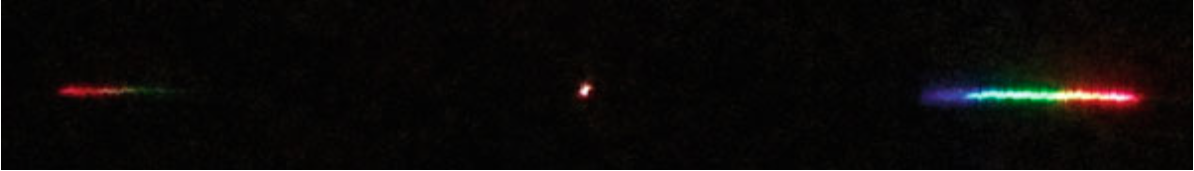
\includegraphics[width=.8\textwidth]{./images/rbw_optics/zero_and_first_order.png}
					\caption{From left to right: Dimmer first order spectrum, zero-order star, and 
							brighter first-order spectrum (Hopkins, 2014\cite{hopkins_spec})}
				\end{center}	
			\end{figure}
	\item Rotate the eyepiece inside the star diagonal so that the spectrum is horizontal from the viewer's perspective
	\item Center the brighter first-order spectrum in the field-of-view and adjust the focus until the spectrum becomes
			as narrow as possible
	\item Place the lens cell centered over the eyepiece and rotate the lens cell until the height of the spectrum is maximized.
			When this is achieved, tighten the thumbscrews.
			The spectrum should appear wider vertically than when viewed through the eyepiece.
			You should begin to see spectral lines.
	\item Adjust the focus again to sharpen the spectral lines by turning the focus knob very slightly counter-clockwise.
\end{enumerate}

You may want to increase the dispersion of the spectrum, ie. the width of the spectrum, and by proxy resolution.
This can be done by inserting spacers to increase the distance between eyepiece lens and the grating cell.
However, this has it's limits. As the dispersion increases, the brightness of the spectrum at a particular wavelength decreases.
Additionally, too much spacing will lead to significant vignetting.
%For example, the combination of the spectroscope, a 25mm eyepiece, and a C8 (F/10, 8'') will be able to fit the zero-order star and
%first-order spectrum in the same field-of-view.
%To expand the image so just the first order spectrum is seen and fill most of the view, a 17 mm or even 12 mm will provide an excellent expanded view of just the first order spectrum.
\par A novel teaching method for introducing spectroscopy is to use the spectroscope with a C8 telescope,
an 18mm eyepiece and a gas discharge tube.
\begin{enumerate}
	\item Place the gas discharge tube roughly fifty feet from the telescope inside a cardboard box.
	\item Cut a narrow, vertical slit in the cardboard box, directly in front of the brightest part of the
		discharge tube on the side facing the telescope.
	\item Focus the telescope, eyepiece, spectroscope combination on the slit.
	\item You should be able to observe the emission spectrum of whatever gas is in the discharge tube
\end{enumerate}

\subsection{Spectroscope + MallinCam Setup}
By combining the Rainbow Optics Star Spectroscope with the MallinCam, one can display or capture
the spectra of dimmer targets with relatively short integration times.
This setup is ideal for outreach to display the spectrum on a monitor for many people to view at once.

\begin{figure}[H] 
	\begin{center}
		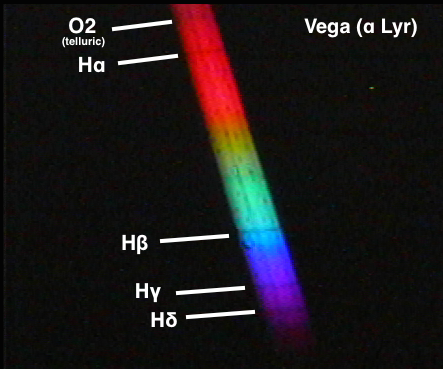
\includegraphics[width=.6\textwidth]{./images/rbw_optics/vega_spec_labeled.png} 
		\caption{A spectrum of Vega collected using the Star Spectroscope, the MallinCam,
				 the MFR-5 focal reducer in the \textit{10mm + "B" + "A"} configuration,
				 and the Meade LX200 telescope. Prominent H-Balmer absorption lines are
				 visible in addition to an atmospheric O$_2$ line.}
		\label{mfr5}
	\end{center}
\end{figure}

\setcounter{rowcount}{0}
\begin{longtable}{c}
	\multicolumn{1}{m{\textwidth}}{\step Follow the procedure in Section \ref{ssec:Astrofest_Setup} to assemble the MallinCam
									and focus on a bright star. (You don't necessarily need to connect a monitor with the 
									frame grabber if you are only trying to capture images of spectra.)} \\
	\multicolumn{1}{m{\textwidth}}{\step Set the MallinCam to a short exposure time (Video Mode) and remove it
									from the star diagonal. Screw the Star Spectroscope onto the end of the 1.25'' adapter or 
									MFR-5
									\footnote[$\dagger$]{If using with a C8, instead screw the grating cell into the threaded end of the star
												diagonal specifically designated for use with the Star Spectroscope.
												Stored on top shelf of telescope room.}.} \\
\end{longtable}\begin{longtable}[t]{cc}
	\multicolumn{1}{m{.5\textwidth}}{\step With the grating cell screwed in completely, the first order spectrum will appear down 
									and to the right of the star. Depending on the dispersion, it may be outside the field of view.
									In order to view the full spectrum, it will have to be horizontal on the chip.
									Through trial and error, remove the MallinCam from the telescope, unscrew the grating cell by a 
									fraction of a turn, reinsert the MallinCam, and check if the spectrum is horizontal. 
									The spectrum will be nearly in focus and appear as a thin line.} 
    & 
    \raisebox{-.5\totalheight}{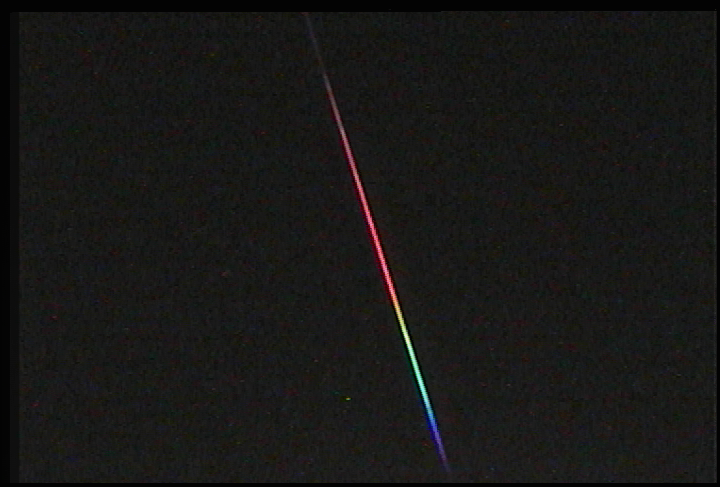
\includegraphics[width=.5\textwidth]{./images/rbw_optics/vega_spec_thin.png}}\vspace{2em}\\
    	\multicolumn{1}{m{.5\textwidth}}{\step Since there is no way to de-focus the spectrum in one dimension with the grating cell when
										using a CCD, we must de-focus the telescope. Turn the telescope coarse adjustment knob until
										the spectrum has widened several times. Spectral lines, if present, should become obvious.} 
    & 
    \raisebox{-.5\totalheight}{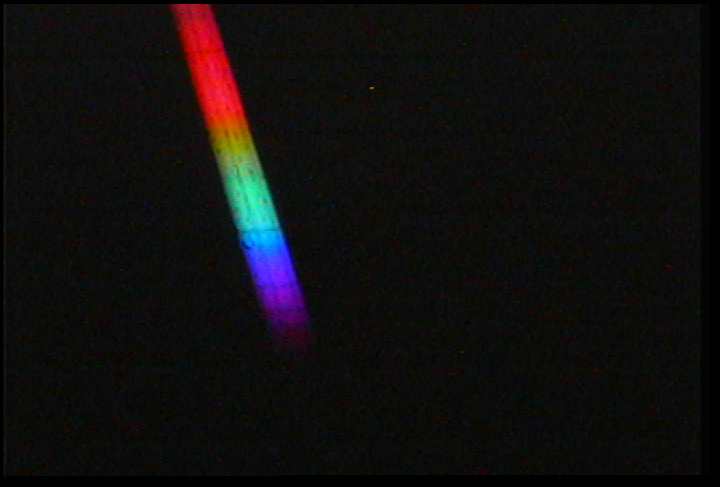
\includegraphics[width=.5\textwidth]{./images/rbw_optics/vega_spec_spread.png}}
\end{longtable} 


\section{Ash Dome}
In the summer of 2013 the roof of ESS was renovated and the original observatory dome was upgraded to a motorized (Model `R') Ash Dome.
This offered a number of improvements, including eliminating the practice of students hanging off of the dome roof in order to open the lower shutter.
The dome features an electrical upper shutter, an electrical winch drop-out lower shutter, and an azimuth drive.
Internet access to the dome is supplied via a 50 ft ethernet cable that runs from an ethernet port outside the telescope room (left wall, just inside blue double-doors), through the adjacent wall, through the roof, emerging from floor of the dome beside the telescope pillar.
Replacing this cable requires removing the south-facing dome stairs to access the hole in the roof beneath the dome floor.
Technical issues with the dome or the Meade LX200 should be addressed to ESS Building Manager, Owen Evans (owen.evans@stonybrook.edu); Dir. of Physics Laboratories, Frank Chin (frank.chin@stonybrook.edu); and/or Machine Shop Dir., Walter Schmeling (walter.schmeling@stonybrook.edu). The Ash Manufacturing Company can be reached at ashdome@ameritech.net or (815) 436-9403.

\subsection{Operation}
\textbf{Do not open the dome if it is raining, snowing, high winds, or if there is snow accumulation on top of the dome.
Never leave the dome unattended while it is in motion.
Never operate the dome with any of the guards removed.
Never allow untrained personnel to operate the observatory dome.
Do not at any time attempt to open or close the upper shutter using the manual override without insuring electrical power is off.
Serious injury may occur.}
%%Is this necessary?
%The dome shutter drive units use a drum switch control.
%The lever action is limited with a safety slide-lock.
%With the lever in the neutral position the slide-lock must be moved manually from either one side or to the other side of the switch.
%This action allows the operator to move the lever from neutral to \textbf{OPEN} or \textbf{CLOSE}.
%The slide-lock causes a forced delay.
\par The dome may be operated either by remote control or the control panels.
When a button is pressed on either the remote or panel and a signal is sent, the yellow light on the panel will turn on.
A five-second time delay is installed into the command system prior to any shutter motions.
The delay is required to prevent any attempt to make an instant change of the shutter's direction without allowing the electrical motor to come to a complete stop.
The motor is not an instant reversing motor and will not reverse direction if it does not stop completely.
The dome will not accept any command it cannot complete.
Any command can be ended immediately by pressing the \textbf{STOP} button.
To reverse any dome motion you must press the \textbf{STOP} button first. 

\subsubsection{Control Panel Operating Instructions}

The shutter control panel is located above the conductor bars to the right of the shutter and the azimuth panel is just below the azimuth motor next to the dome power switch.

\begin{figure}[H]
    \centering
    \begin{subfigure}[t]{0.4\textwidth}
        \centering
        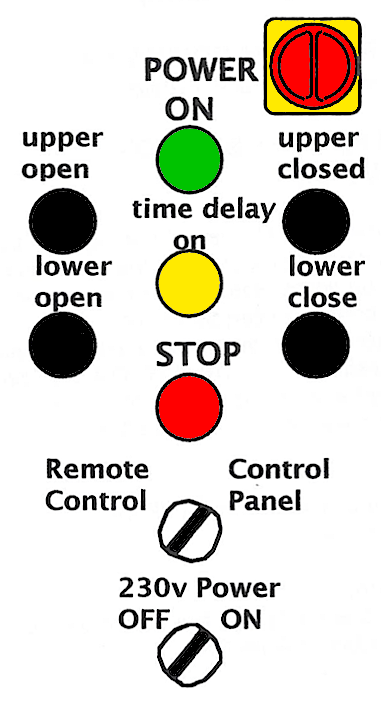
\includegraphics[width=.8\textwidth]{./images/dome/shutter_ctrl_panel.png}
        \caption{Shutter control panel}
    \end{subfigure}%
    \begin{subfigure}[t]{0.4\textwidth}
        \centering
        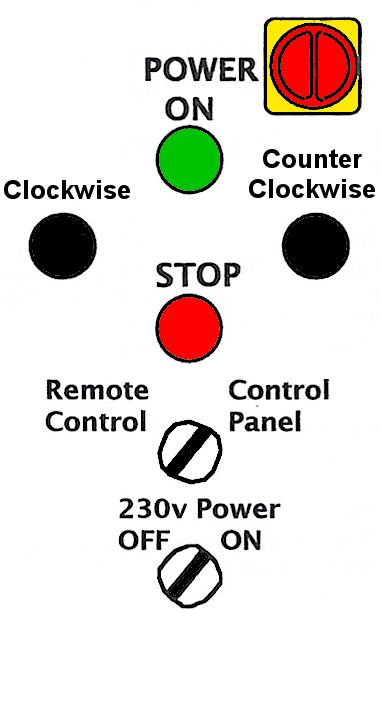
\includegraphics[width=.8\textwidth]{./images/dome/azimuth_ctrl_panel.png}
        \caption{Azimuth control panel}
    \end{subfigure}
    \caption{}
\end{figure}

\begin{enumerate}
	\item Flip the dome power switch to the \textbf{ON} position.
	\item Turn the switch on both control panels from Remote Control to Control Panel
	\item Wait 15 seconds for the time delay to clear system and reset. The green light should turn on.
	\item The upper shutter will open at any time but will not close until the lower drop-out is completely closed.
	\item The shutter can be stopped/started at any point between full open and full close.
	\item The lower shutter will not activate until the upper shutter is raised past the past the safety limit switch (approx. 16'').
\end{enumerate}

\subsubsection{Remote Control Operating Instructions}
There are two dome remotes.
One is kept in the SBIG STL-1001E CCD box in the telescope room and the other in the cabinet inside the dome.

\begin{figure}[H] 
	\begin{center}
		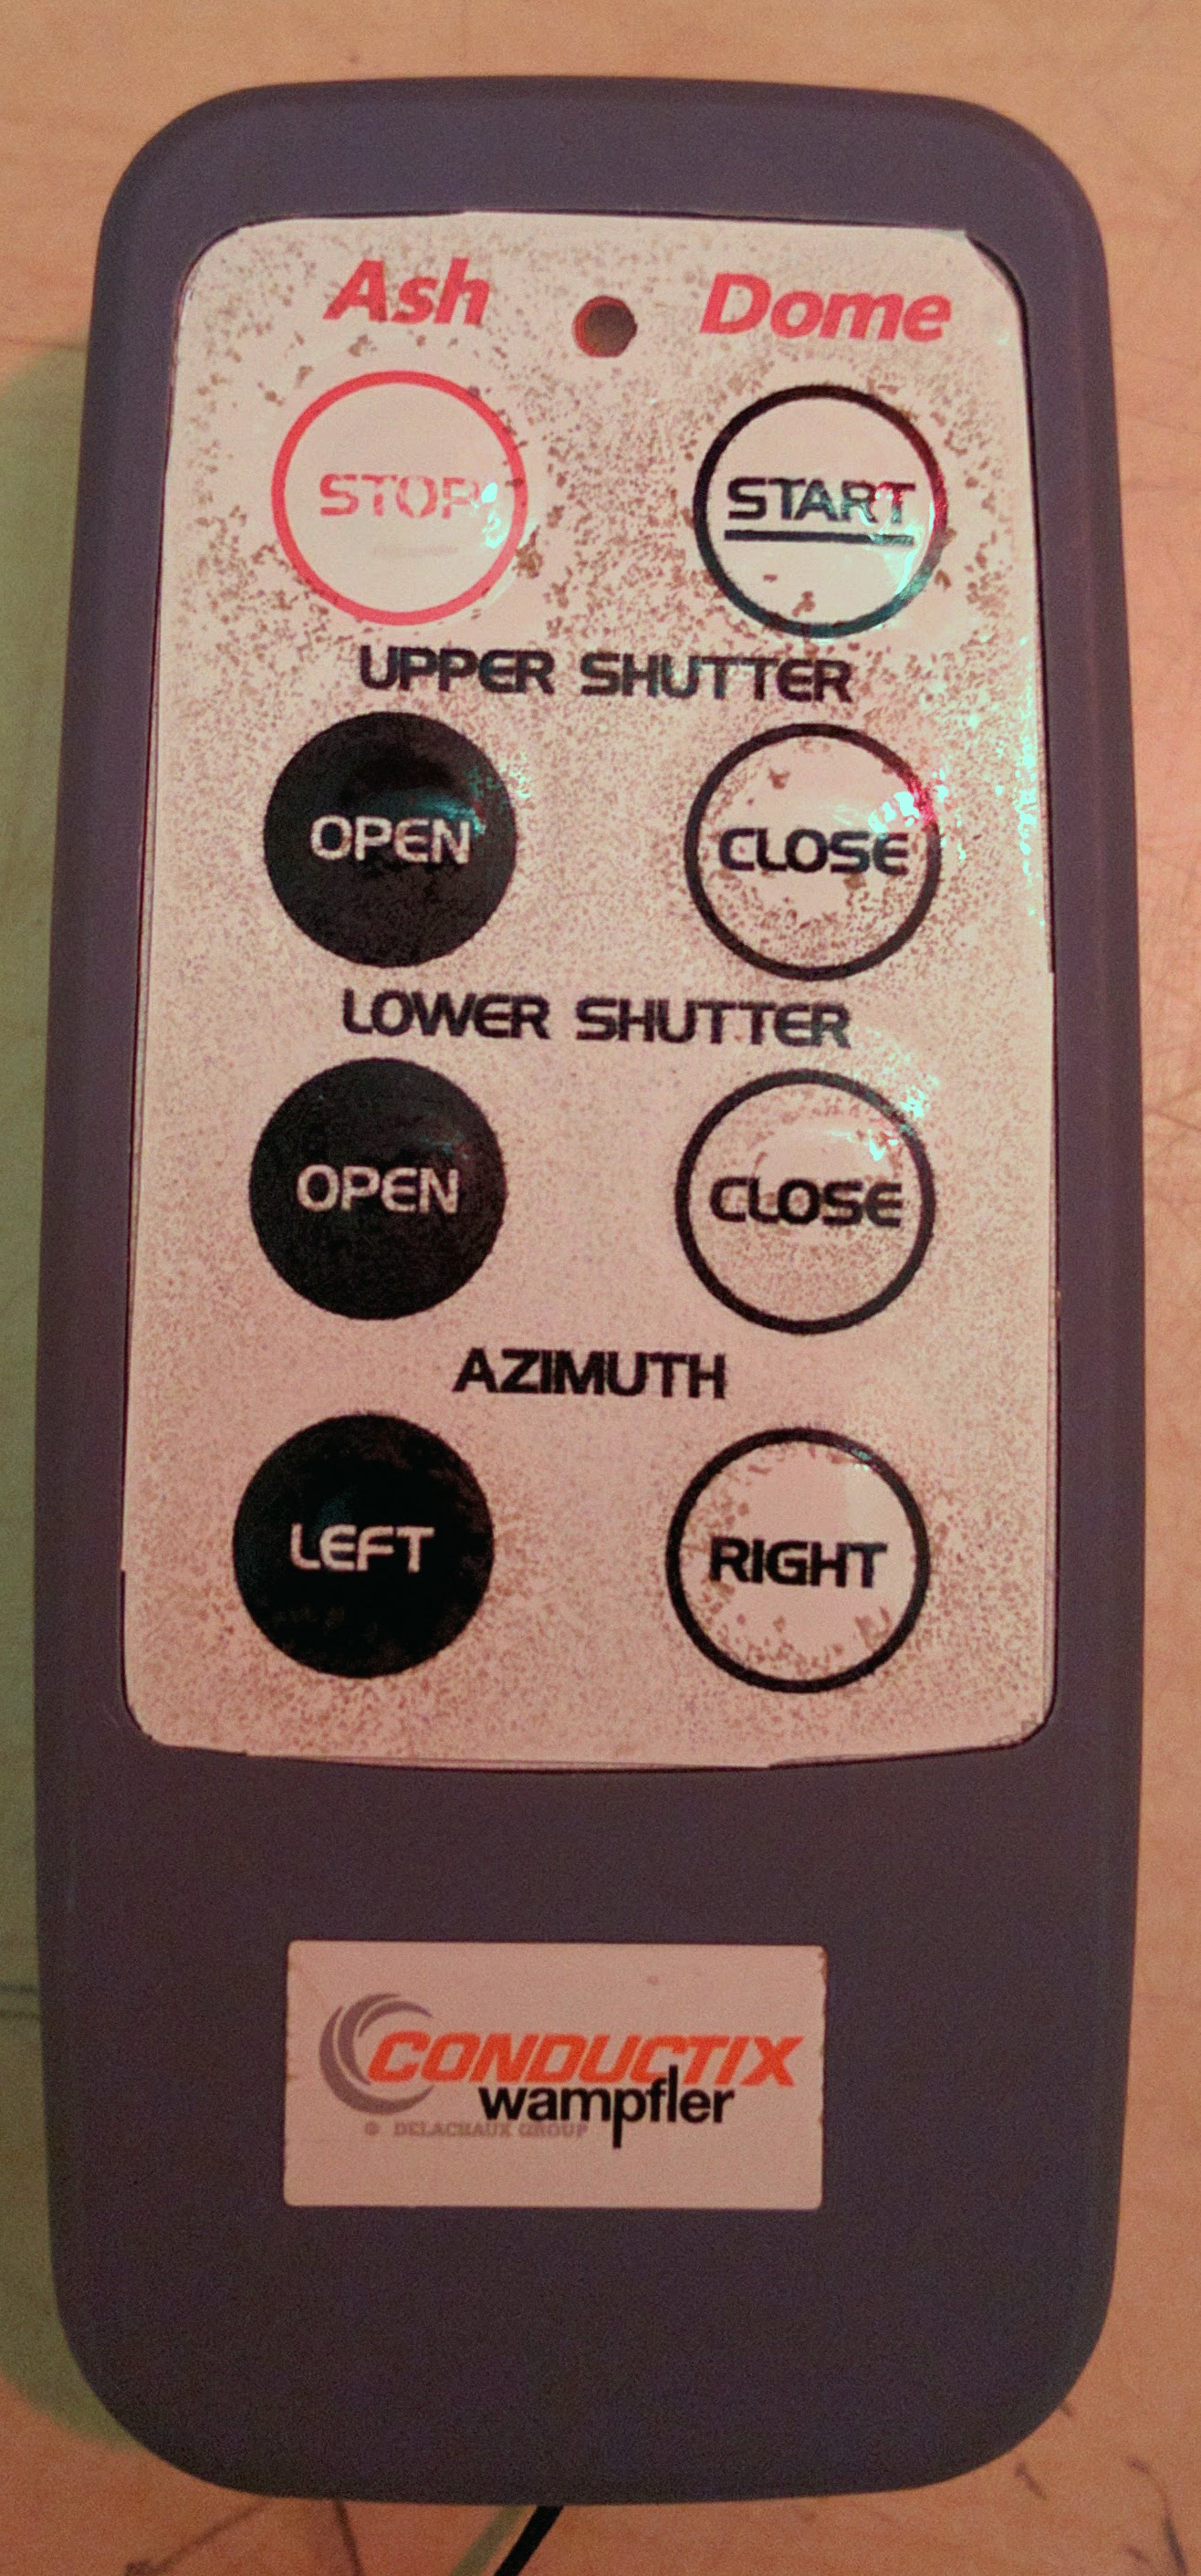
\includegraphics[width=.25\textwidth]{./images/dome/dome_remote.jpg} 
		\label{dome_remote}
	\end{center}
	\caption{Dome remote control}
\end{figure}

\begin{enumerate}
	\item Flip the dome power switch to the \textbf{ON} position.
	\item Turn the switch on both control panels from Control Panel to Remote Control.
	\item Wait 15 seconds for the time delay to clear system and reset. The green light should turn on.
	\item Press and hold the \textbf{\underline{START}} button. The green light on the remote will blink. The system is activated.
	\item Every remote command must be preceded by pressing \textbf{\underline{START}}.
	\item When finished operating in remote control mode, push the \textbf{STOP} button on the remote to shut the system down.
\end{enumerate}

\subsection{Maintenance}
With regular maintenance the Ash Dome should provide many years of service.
The Ash Dome is a positive rack and gear drive system in the shutter and azimuth drives.
These require attention and it is suggested that a regular maintenance schedule should be followed. 
The following activities should be performed bi-annually to prevent wear, incessant squeaking, and maintain peak dome operation:

\setcounter{rowcount}{0}
\begin{longtable}{c}    
    \multicolumn{1}{m{\textwidth}}{\step Apply white lithium grease with a paintbrush to the shutter drive gear teeth and the worm gear.
    										Apply any 3-in-1 oil (or WD-40 in a pinch) to azimuth drive gear teeth.
    										This will usually alleviate most of the squeaking coming from the azimuth track during operation.} \\
    \multicolumn{1}{m{\textwidth}}{\step The edges of the shutter drive track should also be greased to minimize wear.} \\
    \multicolumn{1}{m{\textwidth}}{\step The Neoprene Weather Seals (black rubber skirt) along each side of the dome aperture, around the azimuth rollers and across the front and back of the shutter should be sprayed with a dry silicone to extend the life of the material.} \\[2em]
    \multicolumn{1}{m{\textwidth}}{\centering 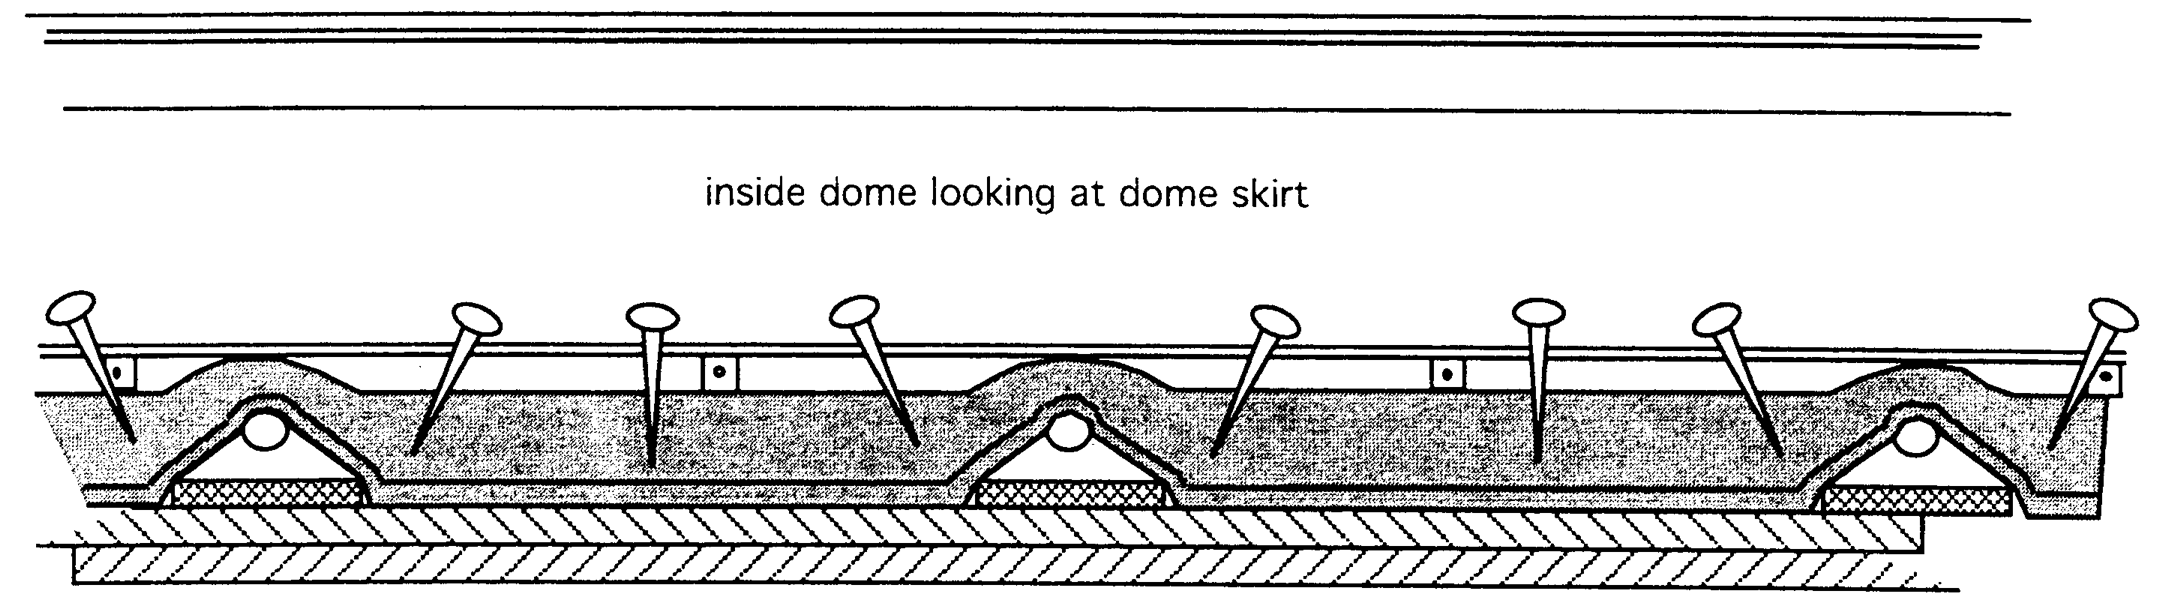
\includegraphics[width=.8\textwidth]{./images/dome/azimuth_skirt_crop.png}} \\
\end{longtable}

\begin{longtable}[t]{cc}
    \multicolumn{1}{m{.5\textwidth}}{\step The dome rotates on steel tires with open bearing rollers.
    The area between the tire and the dome track should be lubricated with any 3-in-1 oil (or WD-40).
    The drive track itself requires no lubrication.} 
    & 
    \raisebox{-.5\totalheight}{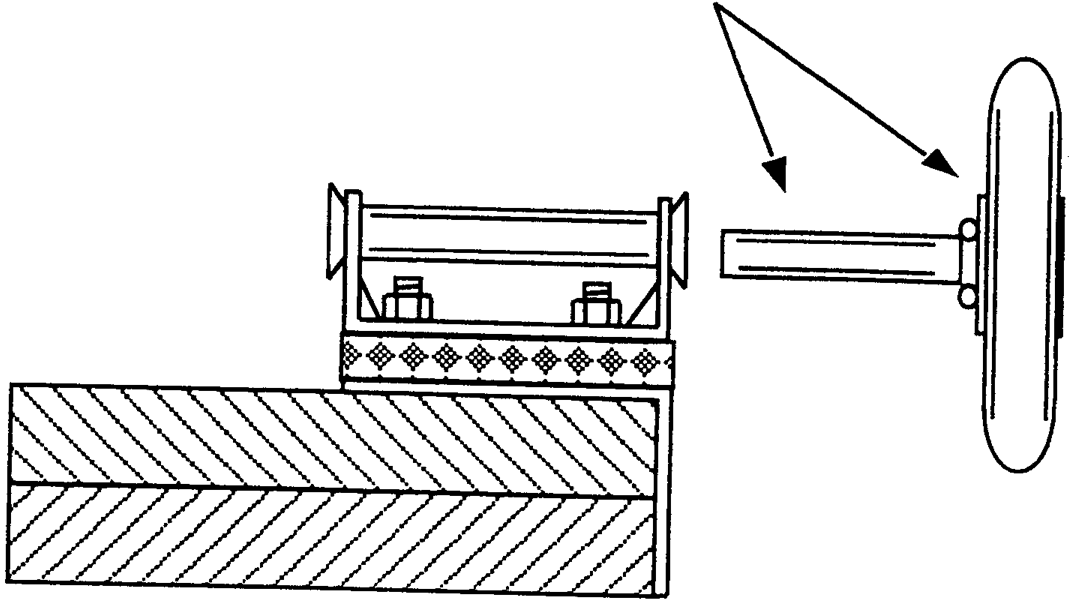
\includegraphics[width=.4\textwidth]{./images/dome/roller_crop.png}}
\end{longtable}

\begin{longtable}[t]{cc}
    \multicolumn{1}{m{\textwidth}}{\step
    The oil levels in the azimuth drive and upper shutter drive gear boxes are filled with Klubersynth UH1 6-460.
    If you do not see any oil leaking it is not necessary to change this oil.} \\     
\end{longtable}

The azimuth drive on Model ‘R’ Ash-Domes may require adjustment over time.
The azimuth drive gear may need to be pressed down further into the drive track.
This is done using the wing nut in the motor mounting bracket.
The azimuth drive system should be adjusted so the gear engages the azimuth drive track just pressing against the track.
The azimuth drive motor mount is spring-loaded and the drive gears more or less floats along in the drive track.
Over tightening of the tension spring and drive gear will promote excessive wear of the drive gear and track.
The drive track itself requires no lubrication.
Ideally, this should be done only by someone from the machine shop.
\begin{figure}[H] 
	\begin{center}
		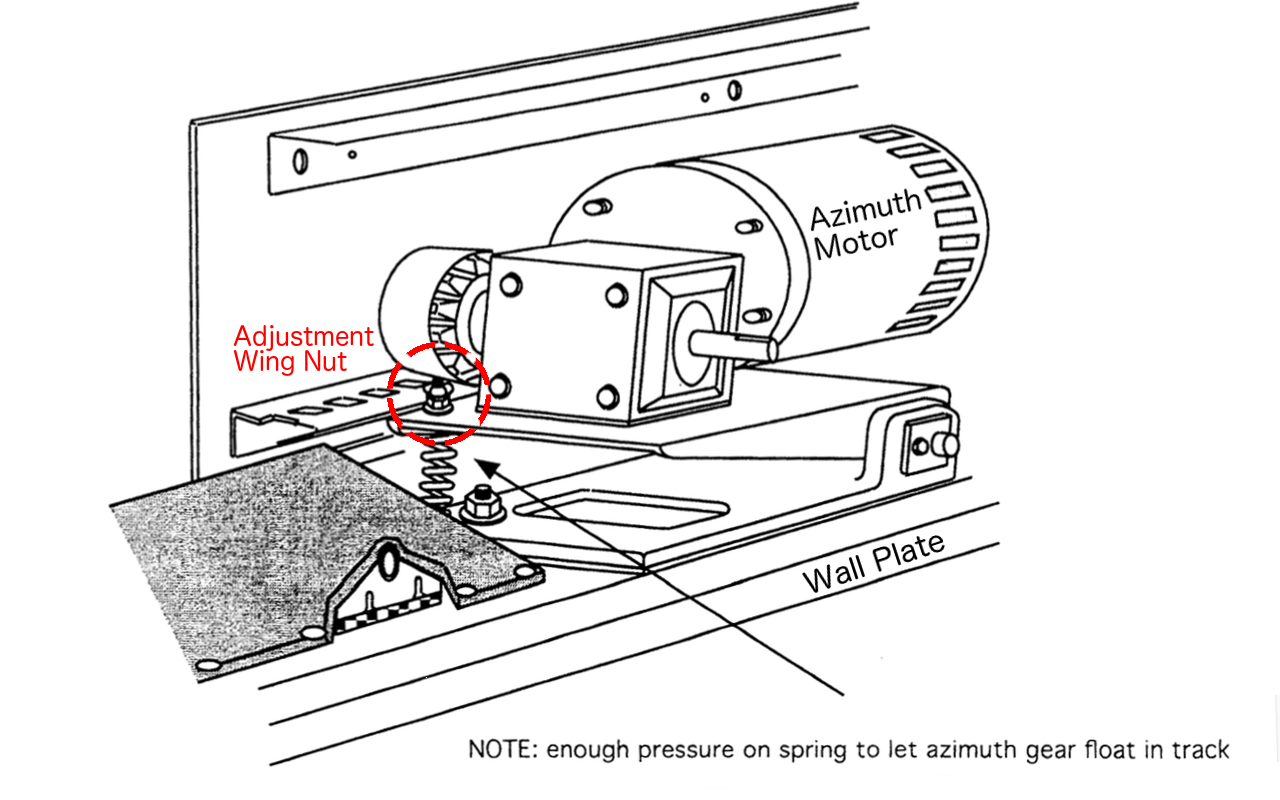
\includegraphics[width=.8\textwidth]{./images/dome/azimuth_motor_wide.png} 
		\label{azimuth_motor}
	\end{center}
\end{figure}

\subsection{Dome and Roof Troubleshooting}\label{ssec:dome_trouble}
\noindent\textbf{Issue:}\\
In the event that the dome loses power, do not leave the shutter open.\\

\noindent\textbf{Solution:}\\
Perform the following actions to close the dome:
\setcounter{rowcount}{0}
\begin{longtable}{c}    
    \multicolumn{1}{m{\textwidth}}{\step Ensure that the main dome power switch is \textbf{OFF}.}
\end{longtable}
\vspace{-2em}
\begin{longtable}{cc}    
    \multicolumn{1}{m{.75\textwidth}}{\step In order to close the lower shutter, you must disengage the spring arm that holds the lower shutter open.
    To disengage the spring arm you must remove the eye-bolt that holds the top hook of the tension spring (pictured)
    by unscrewing the nut on top of the L-bracket.
    There are monkey wrenches in the dome cabinet.
    The location of the spring and bolt in the context of the entire lower shutter is shown in Figure \ref{apdx:lower_shutter}.
    If the lower shutter is fully open then there should be no tension on the spring and it should come off easily.}
    & 
    \raisebox{-.5\totalheight}{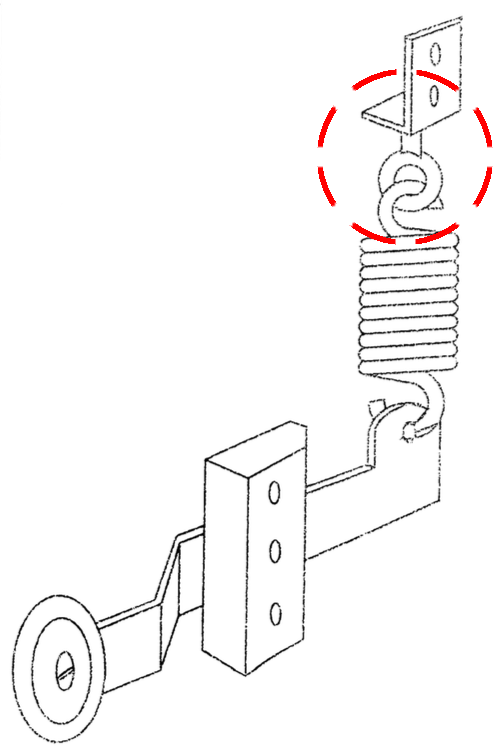
\includegraphics[width=.2\textwidth]{./images/dome/spring_arm.png}}
\end{longtable}
\vspace{-2em}
\begin{longtable}{c}    
    \multicolumn{1}{m{\textwidth}}{\step Reel the lower shutter in by the cable. 
    The lower shutter must be closed first.
    Make sure that the disengaged arm and spring do not get jammed between the dome and door.}
\end{longtable}
\begin{longtable}{cc}    
    \multicolumn{1}{m{.75\textwidth}}{\step The upper shutter can be closed fairly easily using the hand crank.
	Hook the hand crank to the eye-bolt on the upper shutter gearbox (pictured) and turn the crank clockwise to close (CCW to open).}
    & 
    \raisebox{-.5\totalheight}{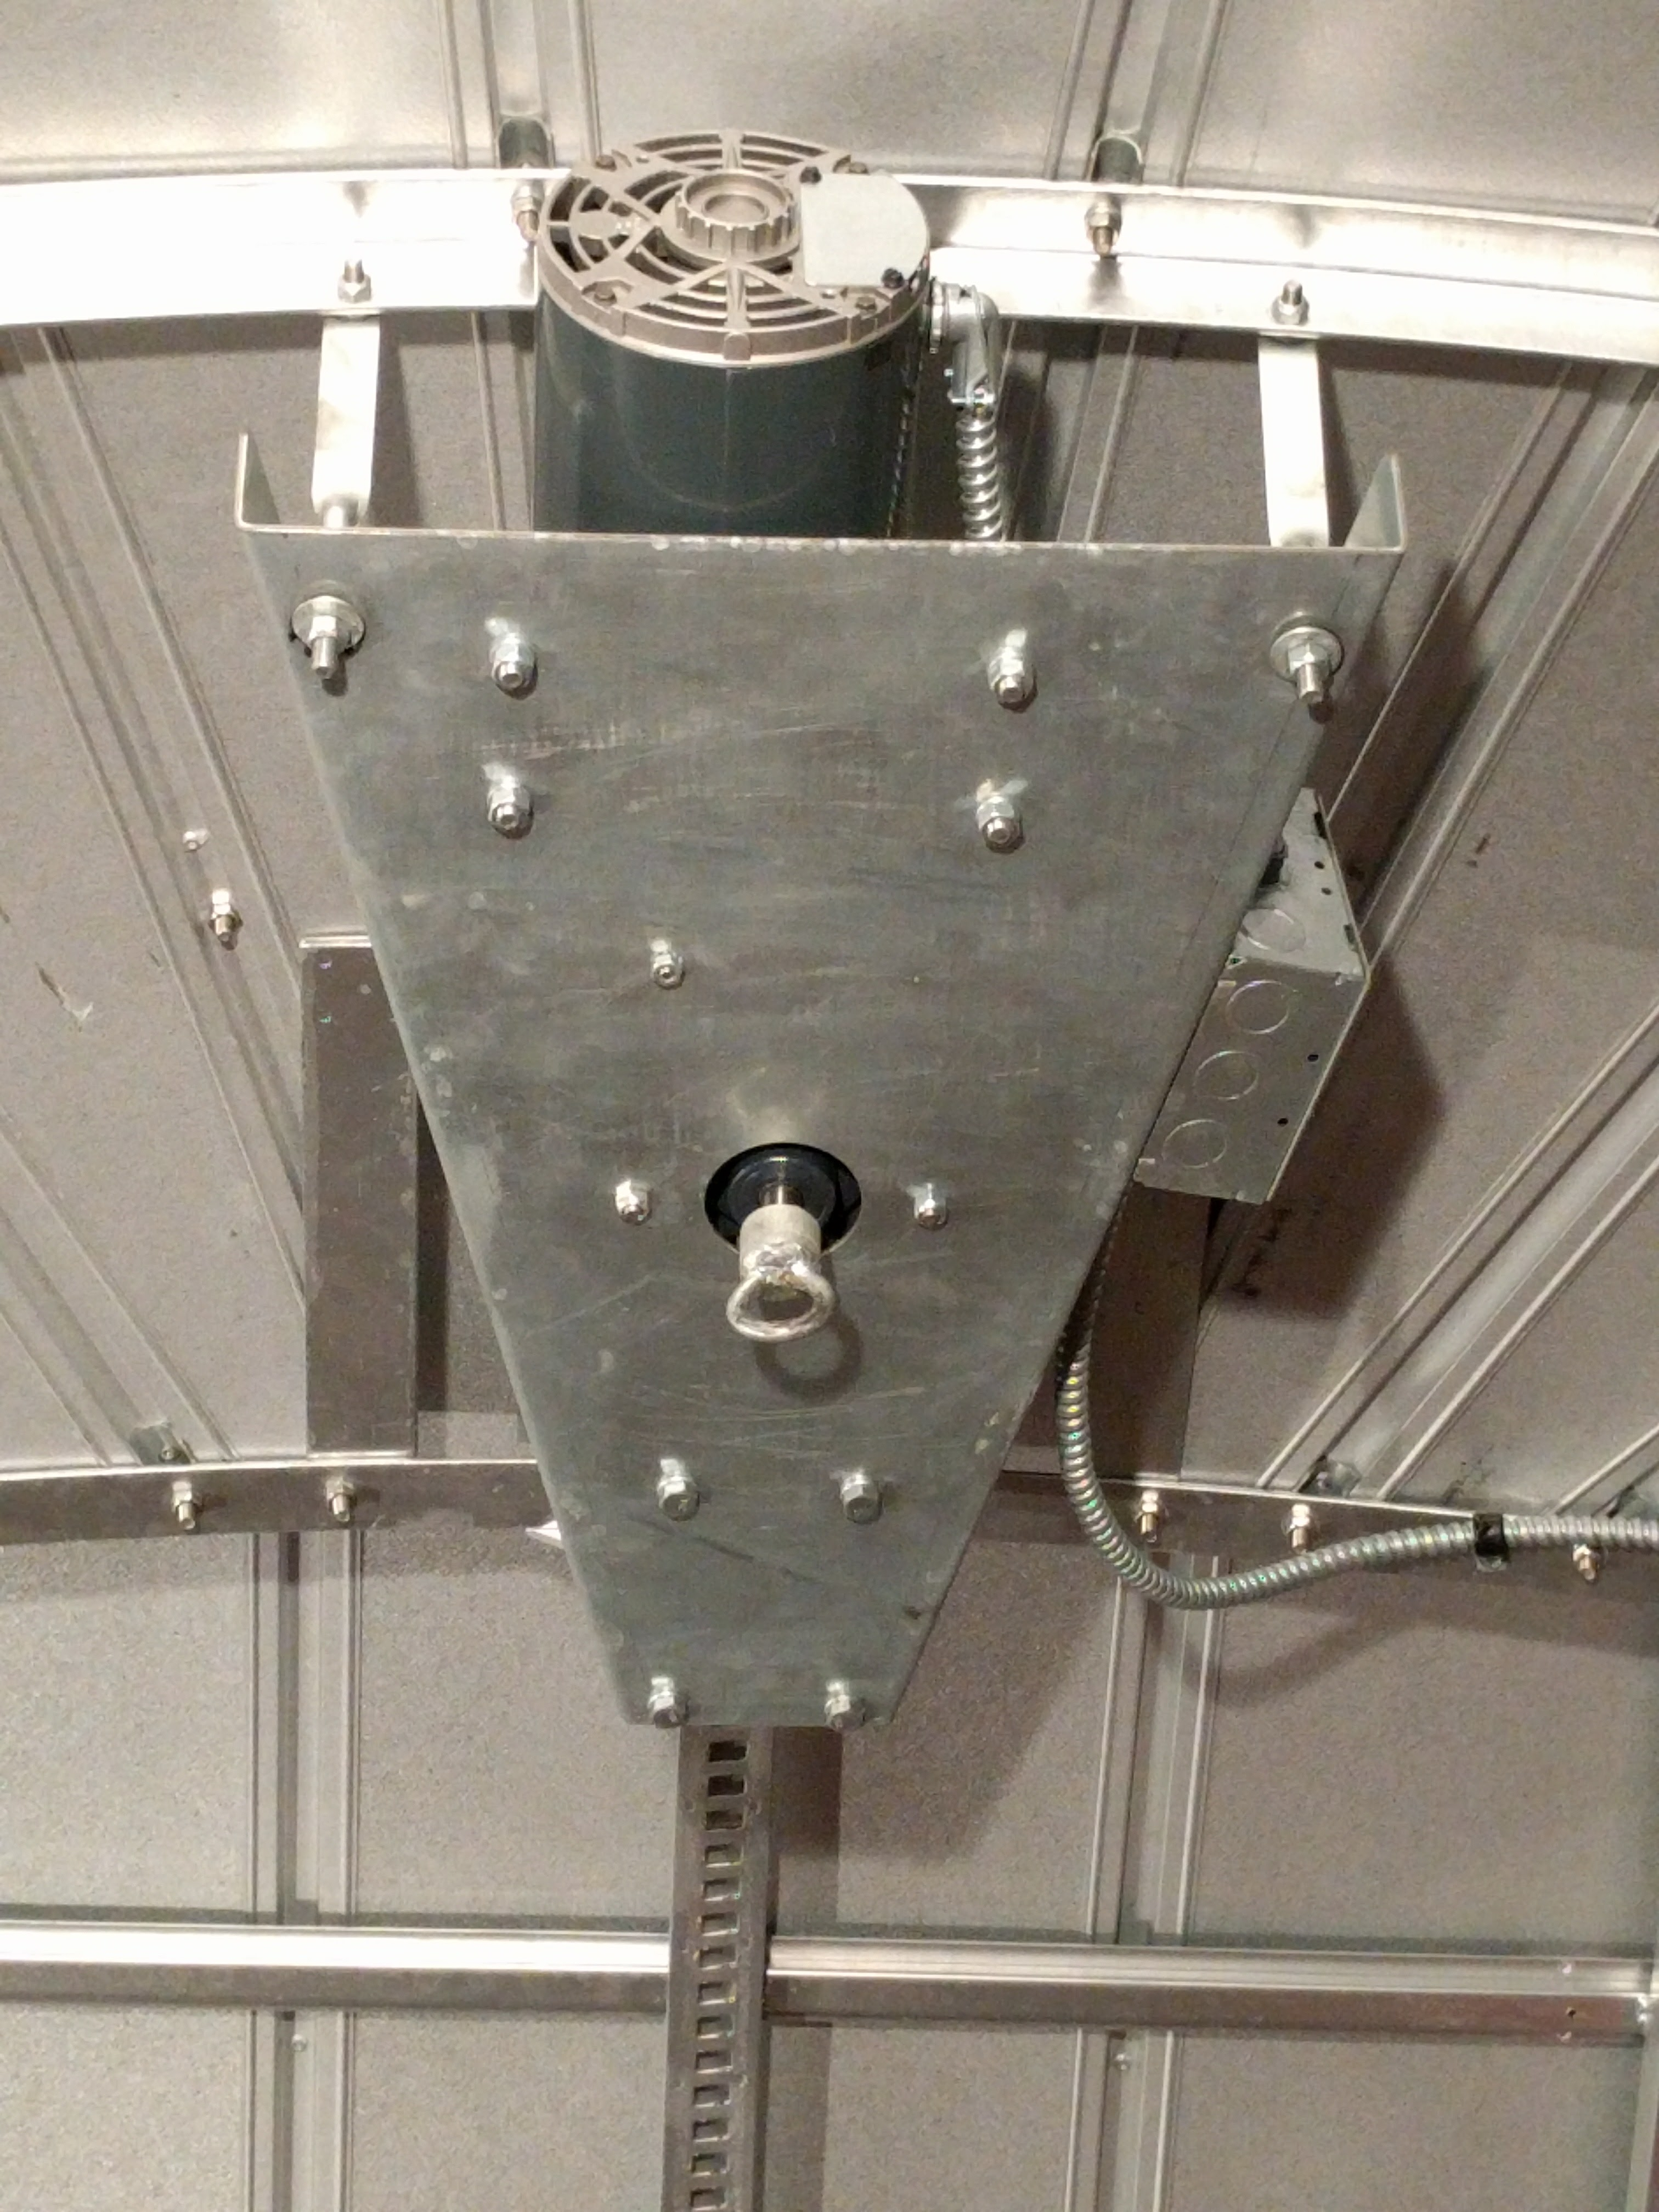
\includegraphics[width=.2\textwidth]{./images/dome/upper_shutter_gearbox.jpg}}
\end{longtable}
\begin{longtable}{c}    
    \multicolumn{1}{m{\textwidth}}{\step Notify the machine shop and building manager.
    They will need to re-wind the lower shutter winch cable.}
\end{longtable}

\noindent\textbf{Issue:}\\
The lights that line the railing on the roof don't turn on.

\begin{longtable}{cc}    
    \multicolumn{1}{m{.5\textwidth}}{\textbf{Solution:} On occasion the switches for the lights that line the railing on 
    									the roof of ESS will appear not to work.
    									Open the cover on the outlet above the light switch near the northern door to the roof.
    									There are two buttons between the two outlets.
    									Press the top button (RESET) followed by the bottom button (TEST).
    									The light switches should now work.}
    & 
    \raisebox{-.8\totalheight}{\includegraphics[width=.5\textwidth]{./images/dome/outlet}}
\end{longtable}

\section*{Acknowledgements}

Thank you to Bent Neilsen from the Physics Labs for letting me (permanently) borrow several small pieces of equipment.
Thank you to Matt Wahl and Stan Metchev for filling in the blanks on some of Betsy's more eccentric behaviors.
Thank you to Larry Faltz and Jack Huerkamp for their extensive help with the MallinCam; helping to troubleshoot issues and recommending maintenance techniques.
Thank you to the Westchester Amateur Astronomers, especially Doug Baum and John Paladini, for their continued support and guidance in imaging techniques and instrumentation.
Thank you to Riley and Jim from Ash Manufacturing for providing schematic diagrams.
Thank you to Owen Evans for giving me free reign after hours and for lending his power tools.
Finally, the construction of this manual would not have been possible without several dedicated
undergraduates who spent many late nights (and occasionally mornings) at the
telescope: Gary Haireti, Blaire Ness, Timothy Sarro, Daniel Welborn, and
Brian J. "Four-Percent" Walker.
Cover photo credit: Jason Berenguer.		

\clearpage





%%%%%%%%%%%%%%%%%%%%%%%%%%%%%%%%%% Appendix %%%%%%%%%%%%%%%%%%%%%%%%%%%%%%%%%%%

\newpage
\begin{flushleft}
\textbf{\Large Appendix}
\end{flushleft}
\begin{appendix}

\setcounter{table}{0}   % Reset table reference counter to zero
\renewcommand{\thetable}{\thesection\arabic{table}}  % Set appendix table titles to 'Table <section><#>'
\setcounter{figure}{0}     % Reset figure reference counter to zero
\renewcommand{\thefigure}{\thesection\arabic{figure}}    % Set appendix figure titles to 'Fig. <section><#>'


\section{Response Curves for SBIG Filters}
...
\section{MallinCam Focal Reduction}
\label{sssec:focal_reduction}
\par The MFR-5 focal reducer consists of four components, shown in Fig. \ref{mfr5} below.
\begin{figure}[H] 
	\begin{center}
		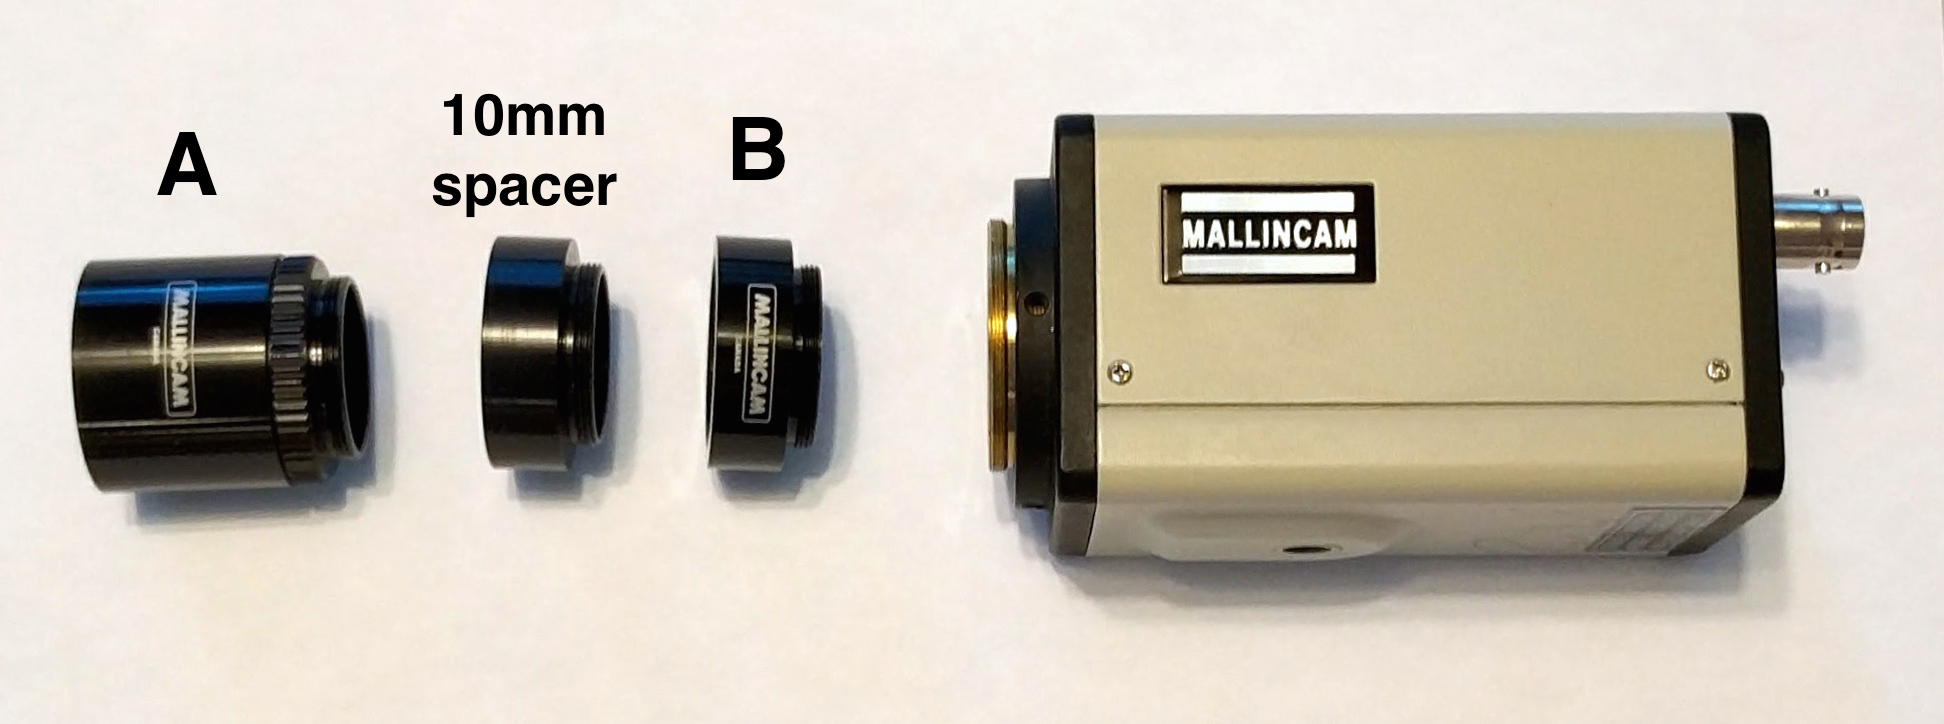
\includegraphics[width=.8\textwidth]{./images/mallincam/focal_reduction/MFR5_labeled.jpg} 
		\caption{The disassembled MFR-5 focal reducer and MallinCam.
				The longer lens will henceforth be referred to as "A" and the shorter, "B".
				The spacers do not contain any optics.}
		\label{mfr5}
	\end{center}
\end{figure}
\noindent Depending on the configuration of these components, the MFR-5 can provide reduction between 0.3x and 0.8x.
Each of the four components are threaded to accommodate 1.25'' filters.
These components can be attached individually or combined to provide more reduction.
However, the "B" ring alone is not long enough to hold the camera inside the telescope so it must be placed between the MallinCam
and the 1.25'' adapter.
\begin{figure}[H] 
	\begin{center}
		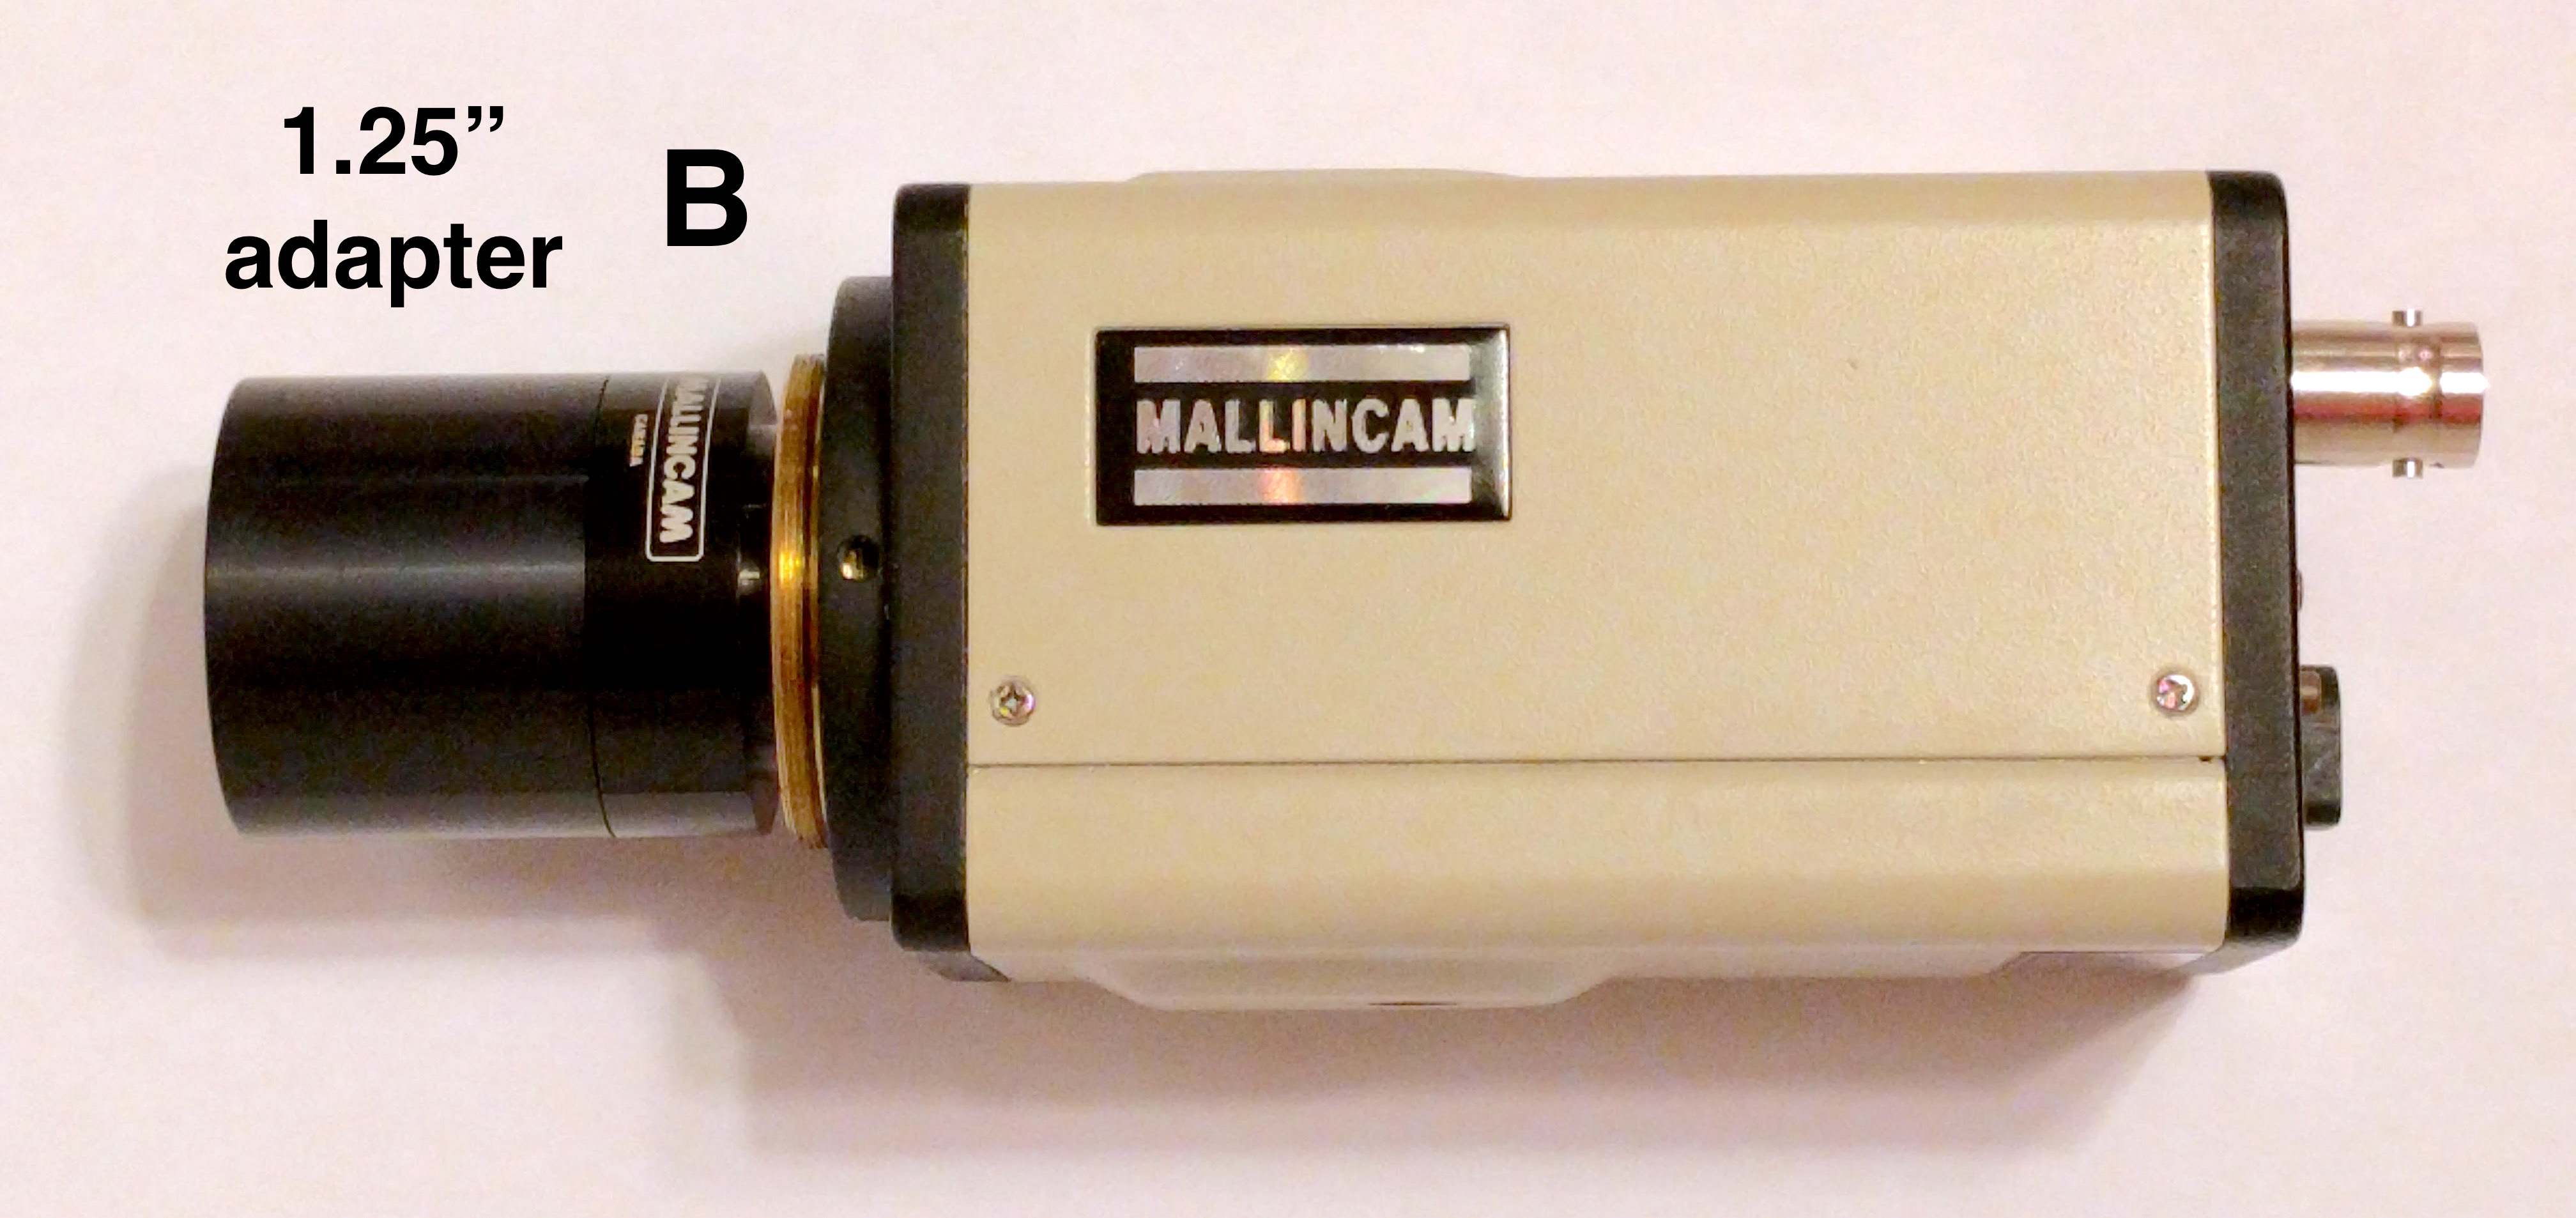
\includegraphics[width=.6\textwidth]{./images/mallincam/focal_reduction/B_adapter.jpg} 
		\label{mfr5_B}
		\caption{This configuration provides 0.8x focal reduction.
				The 1.25'' adapter does not contain any optics.}
	\end{center}
\end{figure}
The following quick-look table provides the focal parameters for all configurations
of the MFR-5 focal reducer and MallinCam on both the LX200 and C8s.
On it's own, the MallinCam behaves like an 8mm objective with a 50$\deg$ apparent field-of-view.

\begin{center}  
\small{
\begin{tabular}{|c|c|c|c|c|c|c|}
	\hline
	\textbf{Configuration} & \textbf{f/ratio} & \thead{\bf reduction\\ \bf factor} & \multicolumn{2}{c|}{\textbf{TFOV (arcmin)}} & \multicolumn{2}{c|}{\textbf{turns to focus}}  \\
										&			&			&	LX200	&	C8		&	LX200	& 	C8 \\ [-1ex]
	\hline
	No focal reducer		 				&	f/10.00	&	1.000	& 	6.75		&	12.00	&			&		\\ [-1ex]								
	\hline
	"B" + "A" 		 					&	f/4.01	&	0.501	& 	13.471	&	23.952	&			&		\\ [-1ex]
	\hline
	5mm + "B" + "A" 	  					&	f/3.27	&	0.409	& 	16.502	&	29.340	&			&		\\ [-1ex]
	\hline
	10mm + "B" + "A" *  					&	f/2.48	&	0.311	& 	21.701	&	38.585	&			&		\\ [-1ex]
	\hline
	"B" + 5mm + "A"   					&	f/3.64	&	0.455	& 	14.833	&	26.374	&			&		\\ [-1ex]
	\hline
	10mm + "B" + 5mm + "A" *$^{\dagger}$ &	f/2.22	&	0.277	& 	24.365	&	43.321	&			&		\\ [-1ex]
	\hline
	"B" 									&	f/6.75	&	0.844	& 	7.997	&	14.218	&			&		\\ [-1ex]
	\hline
	5mm + "B"							&	f/6.29	&	0.786	& 	8.587	&	15.267	&			&		\\ [-1ex]
	\hline
	10mm + "B"							&	f/5.80	&	0.725	& 	9.309	&	16.552	&			&		\\ [-1ex]
	\hline
	15mm + "B"							&	f/5.30 	&	0.662	& 	10.195	&	18.127	&			&		\\ [-1ex]
	\hline
	"A" 									&	f/5.46	&	0.683	& 	9.882	&	17.570	&			&		\\ [-1ex]
	\hline
	5mm + "A" 							&	f/5.10 	&	0.638	& 	10.579	&	18.809	&			&		\\ [-1ex]
	\hline
	10mm + "A"							&	f/4.69 	&	0.587	& 	11.498	&	20.443	&			&		\\ [-1ex]
	\hline
	15mm + "A"							&	f/4.29	&	0.536	& 	12.592	&	22.388	&			&		\\ 
	\hline
\end{tabular}}\\
\captionof{table}{F/ratio, reduction factor, true field-of-view, and 
				coarse adjustment knob turns (to focus from a 40mm eyepiece)
				for each configuration of MallinCam, MFR-5, and telescope.
				The configurations are described listing components from closest to
				furthest from the window of the MallinCam. Configurations
				identified with an asterisk or dagger may result in significant 
				vignetting or coma respectively, especially on smaller scopes.
				F/ratio and reduction factor measurements were obtained from Thompson,
				2013 \cite{thompson13}.}
				\label{tab:focal_reduction} 
\vspace{.4 cm}
\end{center}



\section{Ash Dome Lower Shutter}

\begin{figure}[H] 
	\begin{center}
		\includegraphics[width=.65\textheight]{./images/dome/lower_shutter_schematic.png} 
		\label{azimuth_motor}
	\end{center}
	\caption{A schematic detailing the components of the lower shutter.
			In the event of power loss, remove the eye-bolt holding the spring marked by
			the dashed circle in order to disengage the spring arm and close the door.}
	\label{apdx:lower_shutter}
\end{figure}


\end{appendix}

%%%%%%%%%%%%%%%%%%%%%%%%%%%%% Bibliography %%%%%%%%%%%%%%%%%%%%%%%%%%%%%%%%%%%%%

\newpage
\nocite{*}
\bibliography{Care_and_Feeding_Mt_SB.bib}{}	
\bibliographystyle{plain}
\clearpage

\end{document}
